\documentclass[a4paper,12pt]{scrartcl}
\usepackage[utf8]{inputenc}
\usepackage{lmodern}
\usepackage[ngerman]{babel}
\usepackage[autostyle=true,german=quotes]{csquotes}
\usepackage[T1]{fontenc}
\usepackage[dvips, final]{graphicx}
\usepackage{geometry}
\usepackage{setspace}
\usepackage{amsmath}
\usepackage{colortbl}
\usepackage{multirow}
\usepackage{afterpage}
\usepackage{wrapfig}
\usepackage{fancyhdr}
\usepackage{ae}
\usepackage[hyphens]{url}

\usepackage[colorlinks=true,urlcolor=blue,linkcolor=black,
citecolor=black
]{hyperref}

\bibliographystyle{unsrt}

\geometry{verbose,a4paper,tmargin=30mm,bmargin=35mm,lmargin=25mm,rmargin=25mm}
\pagestyle{fancy}
\renewcommand{\sectionmark}[1]{\markboth{#1}{#1}}
\renewcommand{\subsectionmark}[1]{\markright{#1}}
\fancyhf{}
\lhead{\slshape \leftmark}
\rhead{\thepage}
\title{Deckblatt}
\author{Matthias Misior}

\begin{document}


\thispagestyle{empty}
\section*{Erklärung}
Hiermit versichere ich, dass ich die vorliegende Arbeit selbstständig verfasst und keine anderen als die angegebenen Quellen und Hilfsmittel benutzt habe sowie wörtliche und sinngemäße Zitate als solche gekennzeichnet habe. Diese Versicherung bezieht sich sowohl auf
Textinhalte sowie alle enthaltenen Abbildungen, Skizzen und Tabellen. Die Arbeit wurde in gleicher oder ähnlicher Form keiner anderen Prüfungsbehörde zur Erlangung eines akademischen Grades vorgelegt.
\\\\
Karlsruhe, den 04. April 2018
\\\\
Matthias Misior \noindent\dotfill

\newpage
\thispagestyle{empty}
\section*{Anerkennungen}
Zunächst möchte ich mich an dieser Stelle bei meinem Betreuer Maximilian Liesegang bedanken und meine Anerkennung ihm gegenüber zum Ausdruck bringen. Seine Fachkompetenz und sein Enthusiasmus haben mich über die gesamte Projektdauer begleitet und waren stets eine große Hilfe und eine wichtige Motivationsquelle für mich. 
\\\\
Des weiteren gilt mein persönlicher dank Frau Professorin Laubenheimer, dessen ständige Erreichbarkeit und schneller E-Mail Verkehr es mir erst ermöglicht haben, diese Arbeit in dieser Form rechtzeitig zum Abgabetermin fertigzustellen. 
\\\\
Zu Guter Letzt gilt mein persönlicher Dank dem gesamten esentri-Team. Das Team hat mich inspiriert, andere Wege zu gehen und ich habe dadurch viel über meine Vorgehensweise sowie über mich selbst gelernt. Die Fachkompetenz und Ratschläge des Teams waren dabei stets eine große Hilfe. Ohne die Unterstützung des esentri-Teams wäre diese Arbeit so nicht möglich gewesen.
\\\\
Ich hoffe ich konnte mit diesen einfachen Worten allen Beteiligten meine Dankbarkeit zum Ausdruck bringen. 

\newpage
\thispagestyle{empty}
\section*{Zusammenfassung}
Die esentri AG mit Sitz in der Technologieregion Karlsruhe ist ein mittelständisches Beratungs-Unternehmen mit den Schwerpunkten Digitalisierung und IT-Systemintegration. 
Das Unternehmen plant dabei seine Projekte agil, transparent und nah beim Kunden.
Um den hohen Ansprüchen dieser Kunden nun gerecht zu werden hat es sich die esentri zur Aufgabe gemacht, den internen Dokumentationsprozess innerhalb der Firma zu verbessern. 
\\\\
Diese Aufgabe erweist sich allerdings Aufgrund der in diesem Feld auftretenden Probleme als schwer greifbar. Das Schreiben von Dokumentationen wird meistens als langweilig und monoton angesehen. Hinzukommt dass das Dokumentieren nichts zum Lösungsansatz eines Projektes beiträgt. Aus diesen und weiteren Gründen wird das verfassen von Dokumentationen von vielen Entwicklern als “Zeitverschwendung” betrachtet. 
\\\\
Um diese Tätigkeit nun für die Mitarbeiter attraktiver zu gestalten und somit die Qualität der Dokumentationen zu verbessern, hat man sich dazu entschieden den Dokumentationsprozess mit Gamification aufzuwerten. Dafür soll sich in die Grundlagen des Gebietes Gamification eingearbeitet werden um zu ermitteln, ob und wie man die aus dem Gamification Bereich stammenden Elemente nutzen kann.


\section*{Abstract}
The esentri AG with their headquarters based in the technology region Karlsruhe is an medium-sized consulting-company with a focus on digitization and IT system integration. The company plans its projects agile, transparently and close to the customer. In order to meet the high demands of these customers, esentri has set itself the task of improving the internal documentation process within the company. 
\\\\
However, this task proves to be difficult to grasp due to the problems encountered in this field. Writing documentation is often considered boring and monotonous. In addition, documenting does not contribute to the solution approach of a project. For these and other reasons, writing documentation is considered a \enquote{waste of time} by many developers. 
\\\\
In order to make this activity more attractive for employees and thus improve the quality of documentation, it was decided to enhance the documentation process with gamification. For this purpose, the basics of gamification have to be studied in order to determine whether and how the elements from gamification can be used.     
\newpage
\thispagestyle{empty}
\tableofcontents
\thispagestyle{empty}
\newpage
\bibliographystyle{unsrt}


\section{Einleitung}
Dieses Kapitel dient als Einstieg in diese Arbeit und soll die Aufgaben, Ziele, Vorgehensweise und das Arbeitsumfeld genauer beschreiben. Dabei wird zwischen Aufgabenstellung und Aufgabenbearbeitung unterschieden. Die Aufgabenstellung lässt sich aus der Thesis Beschreibung ableiten und beschreibt die Aufgaben die im laufe dieser Thesis bearbeitet werden sollen. Die Aufgabenbearbeitung enthält die generelle Vorgehensweise wie diese Aufgaben umgesetzt werden. Des Weiteren werden die Ziele definiert, die mit dieser Arbeit erreicht werden sollen. Die Arbeitsumgebung wird ebenfalls beschrieben und es wird am Ende dieses Kapitels mit einem Überblick abgeschlossen. 
\subsection{Aufgabenstellung}
Die Aufgabe die in dieser Arbeit behandelt werden soll ist, die Tätigkeit der Wissenserfassung (Knowledge Capturing) für die Mitarbeiter der esentri AG motivierender und belohnender zu gestalten. Hierfür soll der Wissenserfassungprozess mit Spiele-Prinzipien und Spiele-Mechaniken versehen werden. Durch die Integration von Spiele-Prinzipien und Spiele-Mechaniken sollen dem Autor (Person die das Wissen erfasst und in die Wiki einträgt) zusätzliche Anreize gegeben werden, Informationen zu sichern und aufzubereiten. 
\\\\
Das Integrieren von Spiele-Mechaniken und Spiele-Prinzipien in nicht Spiel-Kontexten, wie in diesem konkreten Fall den Wissenserfassungsprozess (WE-Prozess), wird als Gamification bezeichnet.
\\\\
Für die Integration müssen die verschiedensten Spiele-Prinzipien und Spiele-Mechaniken, welche als Gamification Elemente zu verstehen sind, untersucht und bewertet werden. Dafür werden im Vorfeld Kriterien festgelegt anhand derer die verschiedenen Gamification Elemente analysiert werden können. Anschließend sollen die ermittelten Gamification Elemente in das Dokumentationstool der esentri AG integriert werden. 

\subsubsection{Definition Gamification}
Der Begriff Gamification wurde im Jahr 2002 von Nick Pelling geprägt, fand zu dieser Zeit aber keine Aufmerksamkeit und hatte auch mit der heutzutage geläufigen Definition wenig zu tun.
\\\\
\enquote{\textit{Gamification is the use of game mechanics and experience design to digitally engage and motivate people to achieve their goals.}}\cite{gamificationDefinition}
\\\\
Erst 2009 wurde die Idee um Gamification wieder aufgegriffen und fand mit der digitalen Medienbranche auch ein vielseitiges Einsatzgebiet. Seit dieser Zeit (2009) sind mehrere verschiedene Geschäftsfelder um die Kernidee der Gamification entstanden wie z.B. der Bereich der \enquote{Serious Games} oder auch das \enquote{e-learning} Umfeld.  

\subsubsection{Nutzen von Gamification}
Dieses Zitat aus dem Film Mary Poppins beschreibt ziemlich präzise die Idee und den Nutzen, die hinter Gamification stecken:\\\\ 
\enquote{\textit{In every job that must be done, there is an element of fun. You find the fun, and - SNAP - the job's a game!}} \footnotemark
\footnotetext{Film Mary Poppins, 1964} 
\\\\
Es geht darum, langweilige und monotone Tätigkeiten durch Gamification Elemente motivierender und interessanter zu gestalten. Dadurch soll zum einen der Anwender inspiriert werden. Zum Anderen sollen die Resultate der Tätigkeit durch engagierte Anwender verbessert werden.

\subsection{Ziel dieser Arbeit} 
Ziel dieser Arbeit soll es sein, die Erfassungsbereitschaft von Mitarbeitern der esentri AG zu erhöhen. Als Erfassungsbereitschaft soll der Wille und die Fähigkeit von Mitarbeitern verstanden werden, Inhalte und Informationen abzusichern und aufzubereiten. Zu diesem Zweck sollen aus dem Bereich der Gamification diejenigen Elemente recherchiert werden, die diesem Ziel am förderlichsten sind. Die Gamification Elemente sollen genutzt werden, um ein Konzept zu entwickeln das verwendet werden kann, um in einem weiteren Schritt einen entsprechenden Prototypen zu entwickeln.
\begin{description}
   \item[Erfassungsbereitschaft erhöhen bedeutet:]~\par
   \begin{itemize}
      \item Den \textbf{Willen/Motivation} der Mitarbeiter erhöhen, Informationen zu erfassen und sie so zu gestalten, dass sie effizient von Dritten verwendet werden können.  
      \item Die \textbf{Fähigkeiten} der Mitarbeiter verbessern, Informationen zu sichern.
   \end{itemize}
\end{description}

\begin{description}
   \item[Durch das beeinflussen dieser beiden Punkte sollte es also möglich sein:]~\par
   \begin{itemize}
      \item Das Schreiben und erstellen von Wissensbasen für den Schreiber interessanter zu gestalten.  
      \item Die Qualität der Wissensbasen zu erhöhen.
   \end{itemize}
\end{description}
Ein weiteres Ziel dieser Arbeit ist es, das Themengebiet rund um \enquote{Gamification} der esentri AG näher zu bringen. Der esentri AG ist es ein Anliegen, mehr über die potenziellen Einsatzmöglichkeiten dieses Themengebietes zu erfahren. Die Gamification Elemente und das entwickelte Konzept können dann genutzt werden um z.B. den Dokumentationsprozess zu verbessern. Hierfür müsste das Dokumentationstool \textit{Confluence} erweitert werden. Diese Arbeit soll anhand des Beispiels des Dokumentationstools aufzeigen, ob es sich rentiert Gamification Elemente in bestehende und zukünftige Projekte zu integrieren.  
\subsection{Arbeitsumgebung}
Die esentri AG mit Sitz in Ettlingen ist eine im Jahr 2002 gegründete Beratungs-Firma, die sich auf die beiden Geschäftsbereiche Digitalisierung und IT-Systemintegration spezialisiert hat. Die esentri ist ein cloudbasiertes innovatives Unternehmen das von sich selbst behauptet:
\\\\
\enquote{\textit{Unser Antrieb ist die Neugier, mit der wir nach den aktuellsten Trends Ausschau halten und mit der wir gerne auch mal über den Tellerrand schauen.}} \footnotemark
\footnotetext{\url{http://www.esentri.com/unternehmen/}}
\\\\
Als solches bearbeitet die esentri neben ihren Geschäften auch verschiedenste interne Projekte die sich mit neuen Technologien, Formaten oder Konzepten auseinandersetzen. Zu diesen Projekten zählt auch diese Arbeit. 
\\\\
Das Unternehmen verwaltet und plant seine Projekte agil und greift hierfür auf die Produktpalette von \textit{Atlassian} zurück. Zu den wichtigsten Atlassian Tools innerhalb esentri zählen unter anderem die Aufgabenmanagementsoftware \textit{Jira} und die \textit{Confluence Wiki}.

\subsubsection{Confluence}
Das Confluence Wiki wird seit 2012 bei der esentri eingesetzt. Wichtige Eigenschaften dieses Tools beinhalten die Möglichkeit, Verknüpfungen zwischen Jira, Bitbucket und weiteren Atlassians Produkten zu erzeugen. Somit ist es einfach möglich, Aufgaben Tickets von Jira mit einer speziellen Confluence Wikipage zu verknüpfen. Das stellt einen großen Vorteil gegenüber anderen Wikitools dar.
\\\\
\enquote{\textit{Confluence ist eine kommerzielle Wiki-Software, die vom australischen Unternehmen Atlassian entwickelt und als Enterprise Wiki hauptsächlich für die Kommunikation und den Wissensaustausch in Unternehmen und Organisationen verwendet wird, aber zunehmend auch als Basis für öffentliche Wikis im Internet zum Einsatz kommt.}} \footnotemark
\footnotetext{\url{https://de.wikipedia.org/wiki/Confluence_(Atlassian)}}
\\\\
Die Atlassian Produkte verfügen zusätzlich über weitere \textit{Addons} und über einen eigenen Marketplace. Somit bleiben die Produkte erweiterbar und können individuell zugeschnitten werden.

\subsection{Aufgabenbearbeitung} 
Um die besagten Ziele zu erreichen, ist es wichtig die Kernaspekte dieser Arbeit zu verstehen, sie zu betrachten und ihre zusammenhänge aufzuführen.
\begin{description}
   \item[Die drei wichtigsten Aspekte dieser Arbeit lassen sich wie folgt einteilen:]~\par
   \begin{itemize}
      \item Wissenserfassung
      \item Gamification
      \item Confluence
   \end{itemize}
\end{description}
Diese drei Bereiche müssen behandelt werden, um die im vorherigen Abschnitt erwähnten Ziele, wie das erhöhen der WE-Bereitschaft (Wissenserfassungsbereitschaft) oder das aneignen von Grundlagen Wissen im Bereich Gamification zu erreichen.
\begin{description}
   \item[Dokumentation]~\par
Unter diesem Aspekt müssen die grundlegenden Fragen beantwortet werden wie:
   \begin{itemize}
      \item Wie sichert man relevante Informationen?
      \item Was sind Merkmale einer solchen Wissensbasis?
      \item Warum ist das erfassen und schreiben von Wissensbasen eine eintönige Tätigkeit?
   \end{itemize}
\end{description}
Diese Fragen müssen als aller erstes untersucht und geklärt werden. Anschließend können dann die Kriterien und Anforderungen an den Bereich der Gamification aufgestellt werden. Diese Kriterien können dann verwendet werden, um den Bereich der Gamification besser einzugrenzen. Dadurch wird das Risiko minimiert, sich im Gamification Bereich zu verlieren. 
\\\\
\textbf{Gamification}\\
Die Kriterien und Anforderungen welche sich aus der Analyse des WE-Prozesses (Wissenserfassungsprozess) ergeben, sollen nun genutzt werden, um die entsprechenden Gamification Elemente herauszuarbeiten. Es wird also untersucht, ob es Elemente im Bereich der Gamification gibt, welche auf die Anforderungen und Kriterien passen.
\\\\
Um die Gamification Elemente und die Anforderungen besser aufeinander abstimmen zu können, ist es wichtig sich ebenfalls die Grundlagen zum Thema Gamification anzueignen. Dabei ist zu beachten, dass sich die Gamification Grundlagen nicht nur in technische Lösungen einteilen lassen. Viel mehr ist auf die Psychologie der Motivation und das erzeugen von Verhalten zu achten. In diesem Fall wollen wir die Gamification nutzen um Mitarbeiter zu motivieren und ihr Verhalten soweit ändern, das sie häufiger Informationen selbstständig sichern.
\begin{description}
   \item[Also müssen folgende Forschungsfragen in diesem Abschnitt behandelt werden:]~\par
   \begin{itemize}
      \item Wie kann man Motivation erzeugen?
      \item Wie kann Motivation genutzt werden?
   \end{itemize}
\end{description}
Wenn diese Fragen geklärt sind, ist es möglich Aussagen darüber zu treffen, welche Gamification Elemente sich in Verbindung mit den Anforderungen am besten eignen würden um die WE-Bereitschaft zu erhöhen.
\\\\
\textbf{Confluence}\\
Die identifizierten Gamification Elemente müssen zu guter Letzt noch in das firmeninterne Dokumentationstool \enquote{Confluence} integriert werden. Die benötigten Kenntnisse wie Confluence zu konfigurieren ist, welche Möglichkeiten der Konfiguration Confluence zu Verfügung stellt und wie aufwendig die Integration der gewählten Gamification Elemente wird, fallen in diesen Teil der Arbeit. 
\\\\
Die Confluence Software ist ein wichtiger Baustein der esentri AG und kann deswegen nicht ohne größeren Aufwand ausgetauscht werden. Deswegen ist es wichtig die Grenzen der Software zu ermitteln. Dadurch ist die Auswahl der Gamification Elemente zwar eingeschränkt, da lediglich Elemente verwendet werden dürfen die sich mit dieser Software auch umsetzen lassen. Trotzdem gibt es Punkte die dafür sprechen Confluence als Dokumentationstool für diese Arbeit zu wählen. So kann der Atlassian Marketplace z.B. nach vorhandenen Gamification-Addons durchsucht werden die bereits Gamification Elemente beinhalten.
\\\\
\textbf{Zusammenhang von Knowledge Capturing, Gamification und Confluence}\\
In dieser Arbeit wird versucht alle Schwerpunkte der einzelnen Themenbereiche Knowledge Capturing, Gamification und Confluence zu betrachten und diese zusammenzuführen. Dadurch entstehen natürlich Abhängigkeiten und Zusammenhänge. So können z.B. die Gamification Elemente erst ausgewählt werden nachdem die Anforderungen an die Elemente aus dem Wissenserfassungsprozess ermittelt wurden. Ebenfalls können diese Elemente nur dann verwendet werden wenn sie sich mit Confluence umsetzen lassen. Durch diese Abhängigkeiten aller drei Bereiche unterscheidet sich diese Arbeit von anderen Arbeiten.
\subsection{Übersicht}
Diese Arbeit teilt sich in drei Teile auf. Im ersten Teil werden hauptsächlich die Grundlagen der wichtigen Aspekte Knowledge Capturing, Gamification und Confluence behandelt. Es sollen Begrifflichkeiten und Definitionen dieser Bereiche aufgeführt und erläutert werden. 
\begin{description}
   \item[Aus dieser Phase werden die folgenden Teilergebnisse benötigt:]~\par
   \begin{itemize}
      \item Aus dem Bereich Knowledge Capturing sollen die Anforderungen und Kriterien für die Gamification Elemente ermittelt werden.
      \item Die Anforderungen werden nun verwendet um aus dem Bereich der Gamification die passenden Elemente zu identifizieren.
      \item Im Confluence Teil muss geprüft werden, ob sich die identifizierten Gamification Elemente auch in Confluence umsetzen lassen. Andernfalls muss nach alternativen Lösungsansätzen geforscht werden.
   \end{itemize}
\end{description}
Als Gesamtergebniss dieser ersten Phase, sind die Gamification Elemente zu verstehen die sowohl den Anforderungen entsprechen und sich auch in Confluence Umsetzen lassen.
\\\\
Im zweiten Teil dieser Arbeit wird die technische Umsetzung beschrieben. Es wird dokumentiert, wie die Confluence Wiki konfiguriert wird und wie die aus Phase Eins erarbeiteten Gamification Elemente in die Wiki zu integrieren sind. Des weiteren sollen in dieser Phase Kennzahlen und Messwerte festgehalten werden. Diese Zahlen sollen genutzt werden um die Veränderung der Wissenserfassungsbereitschaft zu messen. Hierfür soll ein einfacher Vergleich von Alter-Zustand zu Neuer-Zustand gezogen werden. Dabei steht der Alter-Zustand für Confluence ohne Gamification und der Neuer-Zustand für Confluence mit Gamification.
\\\\
Im letzten Teil dieser Arbeit sollen die Ergebnisse aus dem Vergleich von Alter-Zustand zu Neuer-Zustand präsentiert und untersucht werden. Diese Bewertung soll Aufschluss darüber geben wie rentable es ist, Gamification Elemente für das konkrete Beispiel des Dokumentationsprozesses zu nutzen. Zum Schluss soll die Arbeit mit einem Fazit und einem Ausblick einblicke in zukünftige Projekte geben.
\newpage
\section{Knowledge Management}
In diesem Kapitel sollen die Grundlagen aus dem Bereich Knowledge Management erläutert werden, die für diese Arbeit relevant sind. Das Thema Knowledge Management ist zu umfangreich um in seiner Gesamtheit für diese Arbeit in Betracht genommen zu werden. Deswegen soll sich in dieser Arbeit nur auf das Knowledge Capturing (Wissen erfassen, dokumentieren) als Untergruppe des Knowledge Management beschränkt werden. Hierzu sollen zunächst die in diesem Kapitel verwendeten Begrifflichkeiten definiert und erklärt werden. Im Anschluss wird beschrieben, was der generelle nutzen des Knowledge Capturing ist und was die Vorteile und Schwierigkeiten dieses Prozesses sind. Des weiteren sollen die Qualitätsmerkmale einer Wissensbasis aufgeführt und anhand von Beispielen erklärt werden. Darauf folgen Gründe, warum Informationen ungerne gesichert werden.
\\\\
Um den Wissensaustausch zu unterstützen muss dieser Prozess zunächst analysiert werden. Hierfür werden Recherchen betrieben die sich mit Knowledge Sharing, Dokumentation, internal Qualität oder ähnlichen Themen beschäftigen. Dadurch sollen Faktoren bestimmt werden, die sich dabei auf den Prozess auswirken. Diese Faktoren werden am Ende als Liste Zusammengefasst und dienen als Überleitung an den Gamification Teil. In den Folgenden Kapiteln wird dann ermittelt, welche Gamification Elemente sich nutzen lassen um die Faktoren positiv zu beeinflussen. Durch diese Beeinflussungen sollte sich dann auch der Wissenserfassungsprozess verbessern.
\\\\
Durch das untersuchen des Knowledge Capturing soll der Bereich aus verschiedenen Perspektiven betrachtet werden. Dadurch sollen nicht nur technische Schwierigkeiten des Wissenserfassungsprozess aufgedeckt werden, sondern vor allem auch die psychologischen Hintergründe, die das Erfassen von Informationen so komplex machen.
\subsection{Definitionen und Begrifflichkeiten}
\label{Definitionen und Begrifflichkeiten}
Hier sind die Definitionen und Begriffe erläutert wie wir sie für diese Arbeit verwenden.
\\\\
Ein \textit{Autor} ist der Verfasser einer Information oder einer Wissensbasis. Der Autor wird meistens der Entwickler sein, da wir uns aber nicht nur auf Software-Dokumentation beschränken, können auch andere Personen wie Technische Schreiber oder Manager als Autoren in Betracht kommen. Ein Autor ist gleichzeitig immer ein \textit{Anwender} der Confluence Wiki und kann in diesem Zusammenhang deswegen auch als solcher genannt werden.
\\\\
Ein \textit{Leser} ist die Person (Entwickler, Stakeholder etc) welche die Information in Confluence liest. Für den Leser wird die Information aufbewahrt. Mehrere Leser werden in dieser Arbeit zusätzlich als \textit{Publikum} verstanden.
\\\\
Eine \textit{Wissensbasis} (Knowledge Base) ist eine Sammlung von Informationen zu einem zusammenhängenden Thema. In dieser Arbeit werden \textit{Dokumentationen} als eine spezielle Form einer Wissensbasis definiert. Eine Dokumentation entspricht nämlich nichts anderes als einer Wissensbasis die sich auf ein Projekt beschränkt. Das heißt alle Informationen des Projektes werden in die Projekt Dokumentation geschrieben. Somit ist eine Dokumentation das Gleiche wie eine Wissensbasis. Wichtig ist letzten Endes nur das die Tätigkeit \textit{Informationen zu erfassen} in den Vordergrund gerückt werden.   
\\\\
Als \textit{Wissenserfassungsprozess} oder \textit{Dokumentationsprozess} (dokumentieren) wird in dieser Arbeit jener Prozess bezeichnet, der für das Sichern von Informationen verantwortlich ist. Dabei wird nicht auf die Art der Information eingegangen um den Begriff universaler in dieser Arbeit verwenden zu können. Des weiteren wird in dieser Arbeit ebenfalls nicht festgelegt, an welchem Ort die Information gespeichert wird. Da in dieser Arbeit die Confluence Wiki als Referenzpunkt genutzt wird, wird in dieser Arbeit aber davon ausgegangen, dass Informationen in diese Wiki eingetragen werden.
\\\\
Der Begriff \textit{technische Schulden} wurde 1992 von Ward Cunningham vorgestellt. Technische Schulden beschreiben dabei den Vorgang, in einem Projekt diejenigen Aktivitäten zu vernachlässigen welche keine neuen Funktionalität in das Projekt bringen. 
\\\\
Zu diesen reduzierten Aktivitäten zählen meistens die Dokumentation des Projektes und das Testen von Funktionen innerhalb des Projektes. Ein Entwickler der an diesem Projekt arbeitet verschuldet sich also, indem Dokumentation und das Testen übergangsweise vernachlässigt werden. Dadurch wird kurzzeitig die Entwicklung des Projektes vorangetrieben. Diese technischen Schulden müssen aber, wie alle Schulden, zu einem späteren Zeitpunkt zurückgezahlt werden. 
\\\\
Die Rückzahlung bei technischen Schulden erfolgt durch das erneute investieren von Zeit, um das Wissen zu erarbeiten, welches während dem Projekt zwar gewonnen wurde, aber nicht rechtzeitig dokumentiert und somit verloren ging. Dies erfordert zusätzliche Anstrengungen die als \textit{technische Zinsen} zu verstehen sind. Die Rückzahlung ist somit teurer als die eigentlichen Kosten für die Dokumentation da die Rückzahlung mit den Zinsen addiert wird.

\subsection{Zweck einer Wissensbasis}
Der Zweck einer Wissensbasis besteht darin, dass relevante Information zu einem Thema gesammelt, gespeichert und aufbereitet werden. Diese Informationen werden aus verschiedenen Gründen erfasst und gespeichert.
\\\\
\textbf{Spätere Verwendung der Information für Autor}\\
Eine Studie von Parnin im Jahr 2010 \cite{Parnin2010} über kognitive Prozesse von Entwicklern beschreibt das Problem im Bereich der Softwareentwicklung: Ein Entwickler dessen Aufgabe darin besteht Quellcode zu generieren verliert schon gleich nach der Implementierung des Codes Informationen die für Änderungen oder Erweiterungen des Codes wichtig wären. Dieses Wissen geht verloren, solange es nicht ausreichend dokumentiert wird. Nach nur wenigen Minuten Ablenkung verliert ein Entwickler bereits seine gut durchdachten Gedankengänge \cite{Graham2004}. Nach wenigen Tagen verblasen Informationen zu ausgewählten Namen und Identifizierern. Nach Wochen verliert ein Entwickler seine Erinnerung an die Mentale Repräsentation die benötigt wird um Aufgaben in Bezug auf den Quellcode zu erfüllen. Es zeigt sich also, dass die menschliche Erinnerung nicht effektiv genug Informationen und Wissen abspeichern kann \cite{Graham2004}.
\\\\
\textbf{Mitarbeiter schneller in das Projekt integrieren}\\
Der Prozess des Onboardings (einen neuen Mitarbeiter in das Projekt einzulernen) ist ein wichtiger Prozess in der IT Branche und besonders bei Beratungsfirmen. Die Fachkenntnisse die in Form von Beratern von Kunden eingekauft werden, bestimmen den Wert der Dienstleistung gegenüber dem Kunden. Mitarbeiter wechseln häufiger nach Bedarf oder Aufgrund von spezifischen Fachkenntnissen die Projekte. Dadurch entstehen zwei Probleme für das Projekt. Verlässt ein Mitarbeiter ein Projekt so verliert es effektiv an Wissen in Form des Mitarbeiters. Wird dieses wertvolle Wissen nicht rechtzeitig gesichert, entstehen finanzielle Kosten. Die Kosten beziehen sich dabei auf erneute Zeitinvestitionen die gemacht werden müssen, um das verlorene Wissen wieder aufzuarbeiten.
\\\\
Zudem sind neue Mitarbeiter mit dem Projekt und dessen Wissenbasis (Dokumentation) nicht vertraut. Das einarbeiten eines Mitarbeiters kostet Zeit und unter Umständen Personal. Um das Einlernen effizienter zu gestalten, ist eine verständliche Wissenbasis unerlässlich. Sie bietet einen Startpunkt in das Projekt für den Mitarbeiter, gibt ihm grundlegende Informationen und ermöglicht ihm Fragen im Vorfeld eigenständig zu beantworten. Desto verständlicher und strukturierter die Wissenbasis, desto effizienter ist der Onboarding-Prozess.   
\\\\
Hinzu kommt das neue Mitarbeiter ihre Probleme effizienter kommunizieren können, da die Kommunikation über die Wissenbasis geführt werden kann. Somit können Senior Mitarbeiter (Mitarbeiter die mit den Projekt gut vertraut sind) einfach auf die Wissenbasis verweisen wenn es Unklarheiten gibt. 
\\\\
\textbf{Erweiterbarkeit des Projektes wird gesichert}\\
Durch eine strukturierte Wissensbasis in Form einer Dokumentation können leichter Änderungen an den Projekten durchgeführt werden. Die Informationen die hierfür aus der Dokumentation genutzt werden verhindern, das Änderungen an der falschen Stelle gemacht werden. Die Informationen helfen ebenfalls zu ermitteln, welche Lösungsansätze bereits versucht worden sind und wie erfolgreich diese waren. Es fällt ebenfalls leichter zu erkennen, ob die verlangten Änderungen umsetzbar sind oder nicht.
\\\\
\textbf{Wartbarkeit der Software wird sicher gestellt}\\
Das Warten und Instandhalten von Software gehört immer mehr zu den Tätigkeiten eines Entwickler. Deswegen ist es auch hier wichtig, eine verständliche Wissensbasis mit entsprechenden Informationen zu haben die erklären, wie die Software oder das System arbeitet. Dadurch können Fehlerquellen eingegrenzt bzw. identifiziert werden. Fehler die häufiger auftreten, können ebenso in die Dokumentation aufgenommen werden wie grundsätzliche Einstellungen und Konfigurationen.
\\\\
\textbf{Nutzen für verteilte Projekte}\\
Die Dokumentation dient bei verteilten Projekten ebenfalls als Kommunikationsmedium. Dies ist ein wichtiger Punkt für die esentri AG da nicht immer alle Mitglieder des Projektes Vor Ort sind und sich dadurch längere und vor allem kompliziertere Kommunikationswege auftun. Durch das Verweisen auf die Dokumentation, können umständlicher Kommunikationskanäle wie Telefongespräche oder E-Mails reduziert werden oder komplett wegbleiben. Obwohl eine Dokumentation es nicht vermag komplett auf Meetings oder Besprechungen zu verzichten, helfen sie doch durch ein gemeinsames Wissensvokabular diese Meetings effizienter zu gestalten. 

\subsection{Die Hürden des Wissenserfassungsprozesses}
Das sammeln von Informationen für eine Wissensbasis ist natürlich ein Aufwand so wie das implementieren von Code auch. Dieser Prozess kostet Zeit und ist aufgrund seiner Komplexität entsprechend schwer greifbar. Die Komplexität beim WE-Prozess rührt daher, das verschiedene Einflüsse in eine Wissensbasis mit einfließen.
\\\\
Zunächst müssen diejenigen Informationen identifiziert werden, welche in eine Wissensbasis aufgenommen werden sollen. Hierfür muss der Autor entscheiden, welche Informationen wichtig oder unwichtig sind. Diese Fähigkeit zu erlangen erfordert Übung und Erfahrung. Das Kategorisieren (Wichtig/Unwichtig) von Informationen ist eine komplexe Angelegenheit, da hier sowohl der Wissensstand des Autors als auch der Wissensstand des Lesers eine entscheidende Rolle spielt. Was für den einen Trivial und ersichtlich erscheint, muss für den Anderen nicht unbedingt ebenfalls so sein. Ist die Wissenslücke zwischen Autor und Leser zu groß, wirkt sich das negativ auf die Qualität der Information und somit automatisch auf die Qualität der Wissensbasis aus. Die Identifizierung und die Kategorisierung von Information kann bis heute noch nicht automatisiert werden, da es bis jetzt noch kein System gib,t dass das menschliche Urteilsvermögen ersetzen kann.
\\\\
Der nächste Faktor in der Komplexität des WE-Prozesses ist die Darstellung der Information. Die Information sollte leicht verständlich, kurz und knapp dargestellt sein. (KISS-Prinzip\footnotemark
). Nicht jeder Autor ist jedoch in der Lage, seine einzigartigen Gedanken so zu formulieren, dass sie als verständlich angesehen werden. Informationen kurz oder knapp zu halten ist ebenfalls nicht so trivial wie man anfangs vermuten lässt. Schließlich müssen Informationen kompakt und auf den Punkt gebracht werden. Die Essenz einer Information zu sichern muss ebenfalls dem menschlichen Urteilsvermögen überlassen werden. Unterstützung durch Tools oder Systeme gibt es auch hier nicht.
\footnotetext{\url{http://www.community-of-knowledge.de/beitrag/keep-it-simple-stupid-leichtgewichtiges-wissensmanagement-mit-wikis}}
\\\\
Die identifizierten und ausformulierten Informationen müssen anschließend in eine Form und Struktur übernommen werden, die logisch und verständlich für das entsprechende Publikum ist. 

\begin{description}
   \item[Dabei gilt es die Wissensbasis so zu designen:]~\par
   \begin{itemize}
      \item Informationen sollten leicht und schnell zu erkennen sein.
      \item Informationen sollten säuberlich voneinander getrennt sein. 
      \item Informationen sollten entsprechend geordnet sein.
   \end{itemize}
\end{description}
Die Komplexität einer Wissensbasis beschränkt sich aber nicht nur auf die entsprechenden Informationen. Jede Wissensbasis muss je nach Publikum und Themengebiet unterschiedlich gestaltet werden. Zwar gibt es Standards und Normen, wie z.B. der arc42-Standard als Dokumentationsstandard für Architekturen. Dennoch können die vielseitigen Sichten nicht alle in einen Standard vereint werden.
\\\\
Hinzu kommt dass das Schreiben von Wissensbasen ein tiefes Verständnis des Themengebietes voraussetzt über das dokumentiert wird. Im Falle der Softwareentwicklung, die hier als Beispiel verwendet werden soll, bedeutet es, dass der implementierte Quellcode verstanden werden muss. Im Idealfall dokumentiert der entsprechende Entwickler selbst den Code, ist dies jedoch nicht der Fall und die Dokumentation wird von einem Dritten geschrieben, gehen schon mal Hintergrundinformationen die eventuell für das Projekt relevant sind verloren. Somit ist es also immer besser, wenn der entsprechende Entwickler einer Funktion oder Komponente (oder ein andere teil des Quellcodes) dessen Dokumentation übernimmt. Dies ist aber nicht immer möglich, da die Zeit fehlt und erfahrene Entwickler mehr damit beschäftigt sind, neue Funktionalität zu implementieren und somit das dokumentieren unerfahrenen Entwicklern überlassen wird. 
\\\\ 
Ein weiteres schwerwiegendes Problem ist auch, dass die Dokumentation einer der ersten Aktivitäten ist, die bei hohen Zeitdruck vernachlässigt wird. Bei Projekten mit einem straffen Zeitplan und näher rückenden Abgabeterminen werden deswegen technische Schulden gemacht um so den vorgegebenen Zeitplan einhalten zu können. Diese Schulden zu erfassen ist schwierig da sie stark kontextabhängig sind. Außerdem müssen ebenfalls die technischen Zinsen erfasst und berücksichtigt werden. Auch diese Angaben sind schwer zu erfassen und somit wird verhindert, dass die gesamten Schulden sachgemäß zurückgezahlt werden können.

\subsection{Vorteile des Wissensaustausch}
\label{Zeitersparnis}
Dennoch zeigen Studien das eine Dokumentation trotz Zeitaufwand und Anstrengungen sich für Firmen rentiert. In einem Experiment von Eirik Tryggeseth zu den Auswirkungen von Dokumentationen auf die Wartung von Software zeigt sich z.B, dass Änderungen an Software Projekten durch Dokumentationen sich effizienter umsetzen lassen. Die Lösungsansätze und Änderungen waren dank Hintergrundinformationen zusätzlich qualitativ besser \cite{Tryggeseth1997}.
\\\\
Bei diesem Experiment wurden zwei Gruppen von Studenten mit Änderungen an einem Software-Projekt beauftragt. Eine Gruppe verwendete dabei eine Dokumentation, während die zweite Gruppe lediglich den Quellcode des Projektes zur Verfügung hatte. Die Gruppe ohne Dokumentation benötigte 21,5 \% mehr Zeit ihre Änderungen umzusetzen als ihre Kollegen die über eine Dokumentation verfügten \cite{Tryggeseth1997}.
\\\\
Das hier erwähnte Experiment zeigt deutlich den größten und wichtigsten Nutzen einer vernünftigen Wissensbasis, das generieren von Zeitersparnissen. Dabei wird sich aber nicht auf die Entwicklungszeit bezogen. Die Entwicklungszeit eines Projektes soll sich in diesem Zusammenhang auf die gesamte Zeitspanne beziehen, welche das planen, implementieren, dokumentieren, testen und in Betrieb nehmen eines entwickelten Projektes beinhaltet. Oder bei Agilen Projekten auf die Zeit aller durchgeführten Sprints. Diese Entwicklungszeit wird natürlich nicht beschleunigt. Die Zeitersparnis macht sich erst dann bemerkbar, Wenn das hier gefundene Wissen in anderen Projekten zur einer Verkürzung deren Entwicklungszeit führt. Dadurch wird das gesammelte Wissen also wiederverwendet und führt dadurch zu einer höheren Qualität von Projekten.
\\\\
Als solches kann eine Dokumentation als Investition in die Zukunft gesehen werden. Die Erfahrungen und das Wissen das bei vergangenen Projekten gewonnen wurde, führt zur besseren Qualität und von einer Senkung der Entwicklungszeit bei zukünftigen Projekten.
\\\\
Ein weiterer Vorteil einer stämmigen Wissensbasis ist das Vermarkten des generierten Wissens. Wie bereits erwähnt ist die esentri AG eine Beratungsfirma. Das Kapital einer Beratungsfirma liegt in den Beratern/innen und deren Fachkenntnisse. Wird das Wissensmanagement ausgebaut und den Mitarbeitern leichter Zugang und ein schnellerer Austausch von Informationen ermöglicht, steigert sich auf lange Sicht gesehen nicht nur die Qualität der Beratungen sondern hebt esentri gegenüber seinen Konkurrenten ab.

\subsection{Qualitätsmerkmale einer Wissensbasis}
In diesem Kapitel soll geklärt, werden was die Merkmaler einer qualitativ hochwertigen Wissensbasis bzw. Dokumentation sind. Diese Merkmale zu verstehen ermöglicht es uns, die konkreten Faktoren zur Beeinflussung des WE-Prozesses zu ermitteln.
\\\\
\textbf{Vollständigkeit}\\
Die Vollständigkeit sagt aus, ob auch wirklich alle Informationen erfasst wurden die für die Wissensbasis relevant sind. Hierbei gilt es für den Autor sich ständig zu entscheiden, welche Informationen sind wichtig, welche nicht. Ist die Information ausreichend oder werden noch weitere Informationen zu einem Punkt benötigt. Letzten Endes ist eine Wissensbasis die Summe ihrer Information \cite{Prause2013}.
\\\\
Fehlen Informationen muss der Leser erst darauf kommen, dass nicht alle Informationen vollständig sind. Das kann er unter Umständen nicht beurteilen und durch das Suchen der entsprechenden Informationen geht wertvolle Zeit verloren.
\\\\
\textbf{Veränderbarkeit}\\
Die Veränderbarkeit sagt aus, wie einfach Informationen ausgetauscht oder modifiziert werden können. Änderungen innerhalb eines Projektes oder eines Produktes müssen natürlich auch in die entsprechende Dokumentation eingetragen werden. Dabei bezieht sich die Veränderbarkeit nicht nur auf technischer Ebene durch Wikis (wie leicht etwas in der Wiki zu ändern ist). Es geht auch darum, an wie vielen Stellen Änderungen in der Dokumentation durchgeführt werden müssen. Desto zentraler und redundanter die Informationen vorliegen, desto leichter und sichere lässt sich die Dokumentation ändern \cite{Prause2013}.
\\\\
\textbf{Aktualität}\\
Ist die Wissensbasis noch auf den aktuellsten Stand? Oder wurden Veränderungen durchgeführt die noch nicht in die Dokumentation erfasst wurden. Es ist schwer alle Änderungen im überblick zu behalten und dafür zu sorgen, das alle Informationen so Aktuell wie möglich sind. Hier gibt es einen Zusammenhang zwischen Aktualität und Veränderbarkeit. Desto Veränderbarer die Dokumentation (liegen Informationen zentral vor), desto leichter ist es die Dokumentation Aktuell zu halten \cite{Prause2013}.
\\\\
\textbf{Eindeutigkeit}\\
Mit diesem Merkmal soll beschrieben werden, wie eindeutig die Informationen innerhalb der Wissensbasis sind. Es geht darum zweideutigkeit zu vermeiden und Missverständnisse zu eliminieren. Eindeutigkeit hilft dem Leser dabei, schnell zu bestimmen, ob die Information für ihn relevant ist und hilft bei der Wissensübertragung \cite{Prause2013}.
\\\\
\textbf{Identifizierbarkeit}\\
Wie leicht können Informationen identifiziert werden und wie macht man sie unterscheidbar. Gleiche Informationen sollten immer in gleicher Form in die Wissensbasis aufgenommen werden. Dadurch lassen sich Informationen anhand Ihrer Form identifizieren anstatt anhand des Inhaltes. Dadurch wird es Lesern erleichtert, die unnötigen Informationen zu überfliegen und die vom Leser benötigten Informationen können schneller gefunden werden \cite{Prause2013}.
\\\\
\textbf{Verständlichkeit}\\
Dieser Punkt ist sehr wichtig. Die Hauptaufgabe einer Wissensbasis ist das Verteilen von Wissen. Eine Wissensbasis muss an dieser Eigenschaft gemessen werden. Die Informationen müssen klar abgeschlossen sein. Sie sollten nicht zu viel Information enthalten da die Aufnahmefähigkeit der Lesser begrenzt ist. Die Informationen sollten nach dem KISS-Prinzip (“Keep it short and simple”) gestaltet werden \cite{Prause2013}.
\\\\
\textbf{Konsistenz}\\
Die Konsistenz beschreibt das Fehlen von Widersprüchen. Eine Wissensbasis ist nur dann verständlich, wenn es keine Informationen gibt die einander widersprechen. Generell sollte eine Wissensbasis immer etwas neues hinzufügen. Gibt es mehrere Informationen die sich widersprechen, müssen diese entfernt werden \cite{Prause2013}.

\subsection{Gründe für die Vernachlässigung des Wissenserfassungsprozesses}
Prause und Dudrik haben 2012 eine Umfrage von Expertenmeinungen durchgeführt. Dabei sollte ermittelt werden, ob die Experten Schwierigkeiten bzw. Probleme bei der Dokumentation und dem Architektur Design in Agiler Software Entwicklung sahen. Desweiteren sollte analysiert werden, was der Ursprung dieser Probleme ist. Dies sollte die Grundlage schaffen um Lösungsansätze für diese Probleme zu entwickeln. Insgesamt wurden in dieser Befragung 37 Experten interviewt \cite{Prause2012}.
\\\\
Diese Befragung bezog sich zwar auf Dokumentationen, da wir aber in Kapitel \ref{Definitionen und Begrifflichkeiten} eine Dokumentation als eine spezielle Wissensbasis definiert haben, können die Ergebnisse der Befragung von Prause und Dudrik auch auf die Gestaltung von Wissensbasen übertragen werden. Die durchgeführte Befragung ergab folgende Ergebnisse wie in Tabelle \ref{ProblemTabelle} zu sehen ist.
\begin{table}[htb]
\begin{tabular}{|l|c|}\hline
\rule{0pt}{15pt}  & \textbf{Experten in Prozent}
\\
\hline
\rule{0pt}{15pt} \textbf{Alle Experten} & 74 \%\\ 
\hline
\rule{0pt}{15pt} \textbf{Experten aus Industrie} & 100 \% \\
\hline
\rule{0pt}{15pt} \textbf{Experten aus Akademia} & 68 \%\\
\hline
\rule{0pt}{15pt} \textbf{Experten des frühen SDLC} & 70 \%\\
\hline
\rule{0pt}{15pt} \textbf{Experten des späten SDLC} & 76 \%\\
\hline
\rule{0pt}{15pt} \textbf{Experten aus der Entwicklung} & 74 \%\\
\hline
\rule{0pt}{15pt} \textbf{Experten aus dem Management} & 78 \%\\
\hline
\rule{0pt}{15pt} \textbf{Experten aus der Theorie} & 66 \%\\
\hline
\rule{0pt}{15pt} \textbf{Experten mit weniger als 5 Jahren Erfahrung} & 88 \%\\
\hline
\rule{0pt}{15pt} \textbf{Experten mit 5 - 10 Jahren Erfahrung} & 82 \%\\
\hline
\rule{0pt}{15pt} \textbf{Experten mit 10 - 20 Jahren Erfahrung} & 71 \%\\
\hline
\rule{0pt}{15pt} \textbf{Experten mit über 20 Jahren Erfahrung} & 40 \%\\
\hline
\end{tabular}
\caption{Experten die ein Problem im Dokumentationsverhalten sahen.}
\label{ProblemTabelle}
\end{table}
Die Tabelle \ref{ProblemTabelle} ist ein Auszug aus der Befragungen der Experten. Die Experten wurden dabei in verschiedene Gruppen aufgeteilt. Die Aufteilung erfolgte dabei nach ihren Tätigkeitsumfeld, Industrie oder Akademisch, nach ihren persönlichen Interesse im Entwicklungslebenszyklus (SDLC steht für Software Development Life Cycle) und nach ihrer Berufserfahrung.
\\\\
Wie in Tabelle \ref{ProblemTabelle} zu sehen ist, gaben viele der Experten zu, Probleme bei der Dokumentation zu sehen. Unabhängig von ihrem Bereich stimmten mehr als 50 \% aller Befragten Experten zu, dass der Dokumentationprozess in Agilen Projekten Probleme bereiten würden. Mit einer einzigen Ausnahme. Nur knapp 40 \% der Experten mit mehr als 20 Jahren Berufserfahrung sahen Probleme beim Thema Dokumentation. Eine mögliche Begründung dafür könnte sein, das Entwickler mit mehr als 20 Jahren Berufserfahrung andere Tätigkeiten in Projekten zugeteilt werden und sie deswegen weniger Probleme sehen als ihre jüngeren Kollegen \cite{Prause2012}.
\\\\
Eine weitere Erkenntnis die in dieser Befragung deutlich wurde ist die Diskrepanz zwischen Industrie und Akademia. Während alle Experten aus der Industrie (100 \%) die Forschungsfrage mit ja beantworteten, gaben nur 68 \% der Experten aus dem Umfeld der Akademia ihre Zustimmung. Dies mag wohl daran liegen, das Projekte in Industrie anderen Standards für Erfolg oder Misserfolg unterliegen.
\\\\
Die Befragung der Experten zeigt, dass die Mängel bei Dokumentationen durchaus nichts ungewöhnliches sind. Sie zeigen ebenfalls deutlich auf, wie komplex und ungreifbar das Problem von mangelnden Dokumentationen ist. Obwohl diese Befragung auf Grundlage von Agilen Prozessen basiert, glauben rund 88 \% der Befragten nicht das diese Probleme ausschließlich in Agilen Projekten zu finden sind. Stattdessen sind diese Probleme sowohl bei nicht-Agilen als Agilen Projekten nachweisbar \cite{Prause2012}. Im nächsten Abschnitt wird betrachtet, welche Ursachen die Experten für die Probleme beim Dokumentationsprozess vermuten.
\subsection{Ursachen für mangelnde Dokumentation}
Als die Experten gefragt wurden, welche möglichen Ursachen dieses Verhalten (Wenig bzw. schlechte Dokumentation) zugrunde liegt, wurden dafür von den Experten verschiedene Gründe genannt. Diese sind in Tabelle \ref{UrsachenTabelle} zusammengefasst. Die Problemursachen die hier erwähnt werden, sind nicht ausschließend Exklusiv. Das bedeutet dass die Experten auch mehrere der Unten aufgeführten Ursachen genannt haben können.
\begin{table}[htb]
\begin{tabular}{|l|c|}\hline
\rule{0pt}{15pt}\textbf{Mögliche Ursachen für mangelnde Dokumentation}  & \textbf{Experten in Prozent}
\\
\hline
\rule{0pt}{15pt} Einige Entwickler legen zuwenig Wert auf Qualität & 49 \% \\ 
\hline
\rule{0pt}{15pt} Einige Entwickler wissen nicht wie sie dokumentieren sollen & 46 \%\\
\hline
\rule{0pt}{15pt} Einige Entwickler haben nicht die Zeit für Dokumentationen & 46 \%\\
\hline
\rule{0pt}{15pt} Dokumentation und Entwurf wird zuwenig beachtet & 46 \%\\
\hline
\rule{0pt}{15pt} Qualitätsziele werden nicht gesetzt & 35 \%\\
\hline
\rule{0pt}{15pt} Einzelner Entwickler hat geringen persönlichen Nutzen & 41 \%\\
\hline
\rule{0pt}{15pt} Andere Projektziele sind wichtiger & 19 \%\\
\hline
\end{tabular}
\caption{Experten geben mögliche Ursachen für mangelnde Dokumentation an.}
\label{UrsachenTabelle}
\end{table}
Die Experten waren der Ansicht (46 \%), dass die Entwickler nicht wissen, wie sie richtig zu dokumentieren haben. Einige Experten (49 \%) waren der Ansicht, das Entwickler nicht genügend wert auf Qualität setzen würden. 46 \% der Experten meinten, es Liege daran, dass die Entwickler entweder keine Zeit hätten sich um Dokumentation zu kümmern oder das sie nicht explizit berücksichtigt würde. Die Experten vermuten auch (35 \%) das Qualitätsziele nicht deutlich genug vorgegeben wurden und der Entwickler deswegen seine Aufgaben nicht erfüllen konnte. Andere Experten glauben, dass zu wenig Vorteile für den einzelnen Entwickler entstehen (41 \%) wenn dieser Dokumentiert und das andere Projektziele (erreichen einer Deadline) wichtiger sind (19 \%) \cite{Prause2012}.
\\\\
Diese sieben Ursachen wurden von den Experten als Begründung für mangelnde oder nicht enthaltene Dokumentation genannt. Wie wir aber bereits am Anfang dieses Kapitel erwähnt hatten, steht für uns das Knowledge Capturing im Vordergrund. Aus diesem Grund sind diese Zahlen und Einschätzungen für diese Arbeit nicht exakt zutreffend. Dennoch geben sie Interessante Einsichten und Ansätze.    
\begin{description}
   \item[So müssen die drei folgenden Ursachen genauer betrachtet werden:]~\par
   \begin{itemize}
      \item Einige Entwickler haben nicht die Zeit für Dokumentationen.
      \item Einzelner Entwickler hat geringen persönlichen Nutzen.
      \item Einige Entwickler wissen nicht wie sie dokumentieren sollen.
   \end{itemize}
\end{description}
Es soll nach den Gründen für diese Ursachen gesucht werden. Durch das genauere Untersuchen dieser Punkte können Ansätze gefunden werden, die beeinflusst werden müssen, um das Verhalten und den Wissenserfassungsprozess zu optimieren. 

\subsection{Faktoren zum beeinflussen des Dokumentationsprozesses}
Wie sich aus den vorangegangenen Kapitel gezeigt hat, besteht für die Mitarbeiter ein zu geringes Interesse sich für den Dokumentationsprozess einzusetzen. Im Allgemeinen tut sich der Mensch schwer, eine Tätigkeit auszuführen die ihm sinnlos erscheint. Und als solche wird der Dokumentationsprozess von vielen Mitarbeitern wahrgenommen. Dies ist nachvollziehbar, wenn man bedenkt dass der größte Vorteil von Dokumentationen, sich auf zukünftige Vorhaben und deren Entwicklung beziehen. Es gibt also zu wenig persönlichen Nutzen für einen Mitarbeiter sich am Dokumentationsprozess zu beteiligen. Dies kann anhand des Verhaltensmodell von BJ Fogg erklärt werden.
\begin{figure}[h!]
\begin{center}
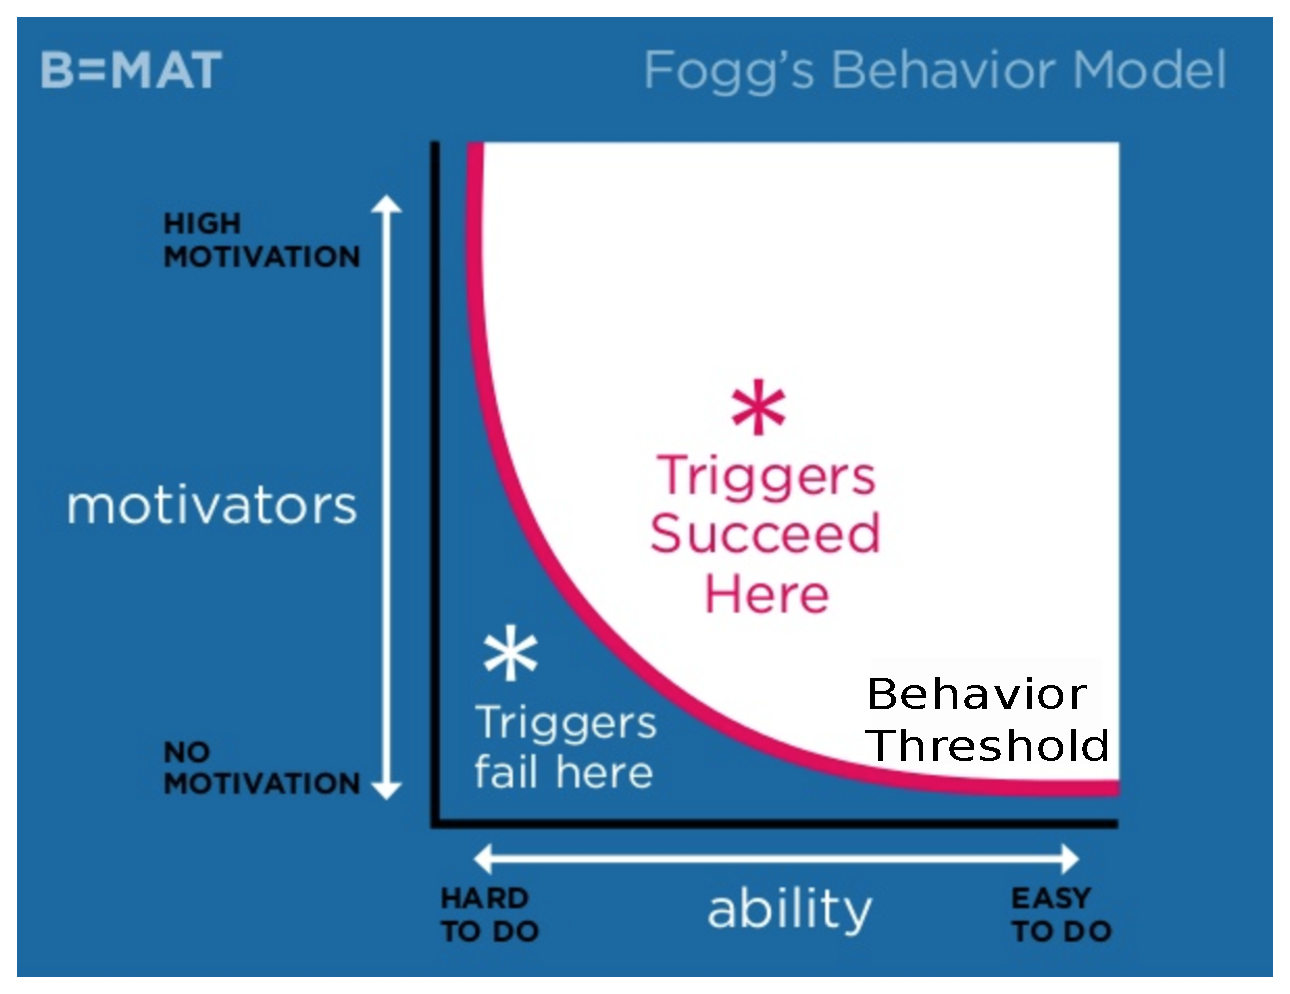
\includegraphics[scale = 0.6]{Bilder/Verhaltensmodell.eps}
\caption{Darstellung des Verhaltensmodell von Fogg \cite{Verhaltensmodell2018}.}
\label{VerhaltensmodellBild}
\end{center}
\end{figure}
\\\\
Das Verhaltensmodell von BJ Fogg (Abb.\ref{VerhaltensmodellBild}) beschreibt die Ursachen für menschliches Verhalten in einer einfachen Formel. Das entsprechende Verhalten ergibt sich aus den drei Teilen, \enquote{motivation}, \enquote{skill} (Fähigkeit) und \enquote{trigger} (Auslöser). Mit diesen drei Punkten lässt sich ermitteln, ob ein Verhalten auftritt oder nicht. Das Modell kann über die einfache Formel \( Verhalten = Motivation + Fähigkeit + Auslöser \) dargestellt werden.
\subsubsection{Verhaltensmodell im Überblick}
Sehen wir uns das Verhaltensmodell, das in Abb.\ref{VerhaltensmodellBild} dargestellt ist, anhand eines einfachen Beispiels an. Das Verhalten \enquote{Bringe Müll raus} würde sich durch das Verhaltensmodell wie folgt darstellen. 
\begin{description}
   \item[Das Verhalten tritt auf:]~\par
   \begin{itemize}
      \item Wenn genügend Lust vorhanden ist, den Müll rauszubringen(Motivation).
      \item Wenn man in der Lage ist, den Müll rauszubringen(Fähigkeit).
      \item Und wenn man merkt das der Müll voll ist(Auslöser).
   \end{itemize}
\end{description}  
Sind alle drei Merkmale (motivation, skill und trigger) vorhanden, tritt das entsprechende Verhalten (Bringe Müll raus) auf. Dabei ist es nicht unbedingt erforderlich, dass das Motivation- und Fähigkeiten-Merkmal immer hoch sein müssen. Es kommt lediglich darauf an ob die \textit{Verhaltensschwelle} (Behavior Threshold) überschritten wird oder nicht (Abb.\ref{VerhaltensmodellBild}). Tätigkeiten die sowohl schwierig umzusetzen sind und bei denen jegliche Motivation fehlt führen dazu, dass die Auslöser für das Verhalten fehlschlagen (Triggers fail here, Abb.\ref{VerhaltensmodellBild}), da hier die Verhaltensschwelle nicht überschritten wird. Dadurch wird das Verhalten nicht hervorgebracht. Das gleiche gilt auch für den umgekehrten Fall. Wird die Verhaltensschwelle überschritten, so wird das Verhalten verursacht. 

\subsection{Die Bestandteile von Verhalten, Motivation, Fähigkeit und Auslöser}
Betrachten wir nun den Dokumentationsprozess als unser vorgegebenes Verhalten (Informationen aufnehmen und speichern), und untersuchen wie dieser Prozess sich auf die drei Merkmale Motivation, Fähigkeit und Auslöser abbilden lässt. Über diese Vorgehensweise wird weitere Einsicht in die menschliche Komponente des Dokumentationsprozesses gewonnen.

\subsubsection{Die Motivation eines Verhaltens}
Die Motivation beim Dokumentationsprozess ist wie wir bereits festgestellt haben sehr gering. Einer der wichtigsten Gründe hierfür liegt wohl daran, dass sich der Nutzen dieses Prozesses erst in der Zukunft bemerkbar macht. Dieser Nutzen zeigt sich anhand eines geringeren Zeitinvestments der Mitarbeiter in zukünftigen Projekten. Das geringere Zeitinvestment wird als solches aber nur gering vom Mitarbeiter wahrgenommen und bietet dem Autor der Dokumentation einen zu geringen persönlichen Nutzen. Menschen bevorzugen aber sofortige und schnelle Gratifikation die sich über diesen Nutzen (geringes Zeitinvestment) nicht erfüllen lässt \cite{Kuhl2009}.
\\\\
Dies erklärt, warum andere Beschäftigungen dem Dokumentationsprozess bevorzugt werden. Da andere Beschäftigungen eine Gratifikation leichter ermöglichen als der Dokumentationsprozess. Da der Nutzen von Zeitersparnis zu unscheinbar und unbefriedigend ist, müssen an dieser Stelle Alternativen eingesetzt werden. Hierfür muss die menschliche Motivation eingehender betrachtet werden.
\\\\
Die Natur der Motivation ist ein umstrittenes Thema in der Forschung und Wissenschaft \cite{Eyal2014}. Um dieses Feld für diese Arbeit Einzugrenzen wird jedoch die Argumentation von BJ Fogg verwendet, da er als einer der führenden Experten in der Verhaltens- und Gewohnheitsforschung gilt. Da sich die Verhaltensforschung mit unserem eigentlichen Ziel überschneidet (Dokumentationprozess als Verhalten zu verbessern), ist seine Argumentation von großer Bedeutung für diese Arbeit. BJ Fogg argumentiert dass es drei Kernpunkte gibt, welche die Motivation in Bezug auf entsprechendes Verhalten ausmacht \cite{Eyal2014}. 
\begin{description}
   \item[Diese Kernprinzipien lauten:]~\par
   \begin{itemize}
      \item Menschen suchen nach Vergnügen und vermeiden Schmerz.
      \item Menschen suchen nach Hoffnung und vermeiden Furcht.
      \item Menschen suchen nach sozialer Akzeptanz und vermeiden Zurückweisung.
   \end{itemize}
\end{description}
Durch die Verwendung und Erweiterung dieser Kernprinzipien \cite{Eyal2014}, kann man die Wahrscheinlichkeit erhöhen, dass eine Person einer bestimmten Aktion nachgeht oder nicht. Im Falle des Dokumentationsprozesses können wir uns auf den ersten dieser drei Punkte stützen, Menschen suchen nach Vergnügen und vermeiden Schmerz. Um dieses Kernprinzip für den Dokumentationsprozess zu nutzen, soll der Begriff des Vergnügens einmal genauer untersucht werden.

\subsubsection{Vergnügen und Belohnung}
Das frühe psychologische Konzept des Vergnügens (Pleasure) und auch das Lustprinzip (pleasure principle) werden als Feedback System gesehen. Im Detail handelt es sich bei Vergnügen um:
\\\\
\enquote{\textit{einen positiven Feedback-Mechanismus, der den Organismus motiviert, in Zukunft die Situation, die er gerade als angenehm empfunden hat, wiederherzustellen und Situationen zu vermeiden, die in der Vergangenheit Schmerzen verursacht haben}} \cite{Freud2015}.
\\\\
Nun muss die Frage beantwortet werden, wie wir dieses Feedback-Mechanismus verwenden können? Die Antwort lautet: Über das bereitstellen einer entsprechenden Belohnung. Denn für die meisten Menschen ist eine Belohnung etwas begehrtes, weil sie eine bewusste Erfahrung des Vergnügens erzeugt \cite{Berridge2009}. Anstelle den Nutzen einer Dokumentation als einzige Motivationsquelle zu verwenden, ist es also erforderlich, eine Alternative, in form einer zusätzlichen Belohnung, zur Verfügung zu stellen.
\\\\
Dabei ist die Art der Belohnung für jeden Menschen anders und damit \enquote{subjektiv}. Wissenschaftler sprechen an dieser Stelle von \enquote{subjektiven Belohnugswerten} \cite{Bonhoeffer2011}. Jeder Mensch misst sich in seinem eigenen Belohnungssystem das ein Teil des Gehirns ist, seine ihm persönlichen Werte zu. Durch die Gamification müsste nun ein generell gültige Belohnung entworfen werden, die für jeden bzw. die meisten Mitarbeiter der esentri AG einen hohen subjektiven Belohnungswert hat. Dadurch würde sich die Motivation steigern lassen und es würde Mitarbeiter eher anspornen sich am Dokumentationsprozess zu beteiligen oder ihn gar von sich aus auslösen.

\subsubsection{Die Fähigkeit ein Verhalten umzusetzen}
Die Fähigkeit beschreibt im Verhaltensmodell von BJ Fogg, ob es sich um eine schwierige oder einfache Aktion handelt aus der sich das entsprechende Verhalten ergibt. In den vorangegangenen Kapiteln hat sich auch hier deutlich gezeigt, das der Dokumentationsprozess mit komplexen Eigenschaften versehen ist, was bedeutet das er in der Fähigkeiten Skala des Verhaltensmodells eher Hoch und damit als schwer einzustufen ist. Wenn unser gewünschtes Verhalten hervortreten soll, ist es erforderlich den Dokumentationsprozess zu vereinfachen. Für die Fähigkeit gibt es ebenfalls Merkmale über die der Schwierigkeitsgrad beeinflusst werden kann.
\begin{description}
   \item[Die Fähigkeitsmerkmale sind:]~\par
   \begin{itemize}
      \item \textbf{Zeit}: Wie lange benötigt man für die entsprechende Aktivität?
      \item \textbf{Geld}: Wie viel Geld kostet die Aktivität?
      \item \textbf{Physical Anstrengung}: Wie anstrengend ist diese Aktivität?
      \item \textbf{Verständnis}: Wie leicht ist die Aktivität zu verstehen?
      \item \textbf{Soziale Abweichung}: Wie viele andere Personen führen die Aktivität aus?
      \item \textbf{Übung}: Wie geübt ist man, die Aktivität durchzuführen?
   \end{itemize}
\end{description}
Diese Fähigkeitsmerkmale sind ebenfalls in Abbildung \ref{FähigkeitsmerkmaleBild} zu sehen. Durch das manipulieren und beeinflussen dieser Fähigkeitsmerkmale, wird der Schwierigkeitsgrad der Aktivität (Informationen speichern) regulierbar. Durch die Reduzierung der Schwierigkeit auf ein niedrigeres Niveau, wird die Wahrscheinlichkeit den Dokumentationsprozess auszuführen gesteigert. Dabei müssen nicht alle sechs Fähigkeitsmerkmale (Zeit, Geld, Anstrengung, Verständnis, Soziale Abweichung und Übung) berücksichtigt werden. Die Merkmale Zeit, Verständnis und soziale Abweichung sollen für diese Arbeit in Betracht gezogen werden. 
\\
\begin{figure}[h!]
\begin{center}
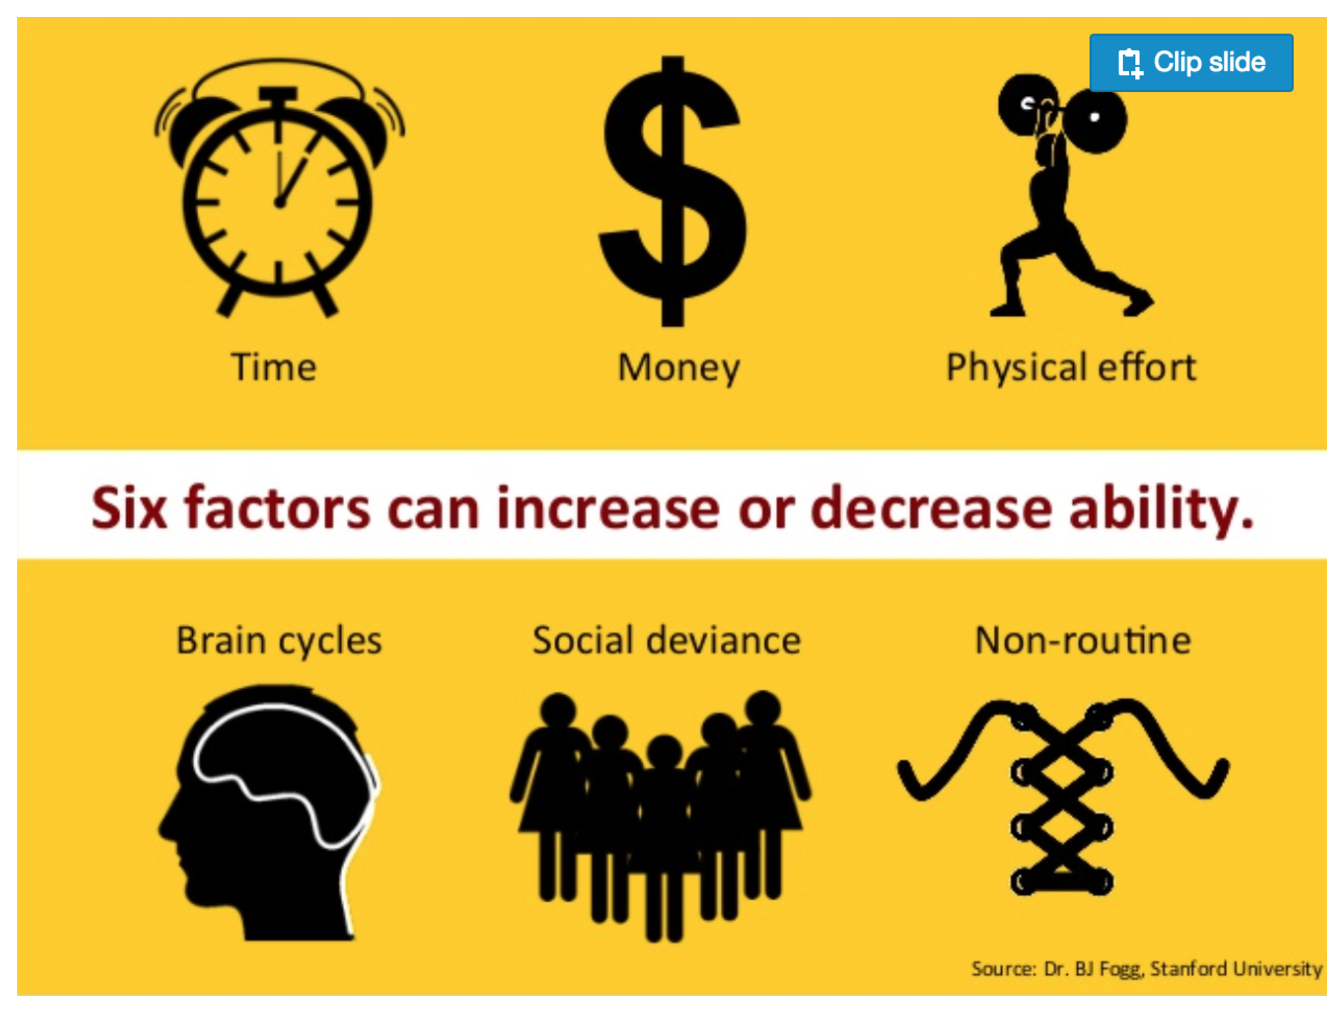
\includegraphics[scale = 0.4]{Bilder/Faehigkeitenfaktoren.eps}
\caption{Darstellung der verschiedenen Fähigkeitsmerkmale \cite{Merkmale2018}.}
\label{FähigkeitsmerkmaleBild}
\end{center}
\end{figure}
\subsubsection{Fähigkeitsmerkmal Zeit}
Zunächst soll das Fähigkeitsmerkmal Zeit untersucht werden. Hier gilt es zu prüfen, ob der Dokumentationsprozess nicht beschleunigt werden kann. Um den Dokumentationsprozess zu beschleunigen, ist es zunächst erforderlich dass der Prozess analysiert wird \cite{Hauptly2008}.\\
\begin{description}
   \item[\parbox{\textwidth}{Um den Dokumentationsprozess sachgemäß zu analysieren müssen die Folgenden Fragen beantwortet werden: \normalfont\vspace{0.5ex}}]~\par
   \begin{enumerate}
      \item Was versucht der Anwender mit dem Dokumentationsprozess zu erreichen?
      \item Welche Schritte müssen vom Anwender unternommen werden, damit er sein Ziel erreicht?
      \item Welche dieser Schritte können entfernt werden ohne vom Ziel des Anwenders abzuweichen?
      \item Welche Schritte können modifiziert werden um sie zu verkürzen?
   \end{enumerate}
\end{description}
Wenn diese Fragen sauber und sachgerecht beantwortet werden können, kann der Dokumentationsprozess optimiert werden. Durch eine Verkürzung der Dauer des Dokumentationsprozesses werden Mitarbeiter eher dazu verleitet, diesen Prozess zu nutzen. Die Analyse des Dokumentationsprozesses wird in kommenden Kapiteln behandelt.

\subsubsection{Fähigkeitsmerkmal Verständnis}
Das Fähigkeitsmerkmal Verständnis kann ebenfalls genutzt werden um den Dokumentationsprozess zu vereinfachen. Sind die einzelnen Schritte des Prozesses erkannt und optimiert, ist es wichtig sie so zu designen, dass sie im Idealfall selbsterklärend und leicht verständlich sind. Dabei ist es notwendig, die Schritte aus denen der Dokumentationsprozess besteht auf ihre kleinst mögliche Handlung zu reduzieren.
\\\\
An dieser Stelle kann zusätzlich die Gamification genutzt werden. Gamification wird nämlich nicht ausschließlich genutzt, um Verhalten zu verändern. Gamification kann ebenfalls genutzt werden, um das erlernen neuer Skills zu fördern. Dies kann nun verwendet werden um den neuen optimierten Dokumentationsprozess für die Anwender zugänglicher zu gestalten.
\\\\
Wie die Gamification sich nun im Detail auf den überarbeiteten Dokumentationsprozess auswirken kann und welche Elemente hierfür verwendet werden sollen, wird in den kommenden Kapiteln erläutert und gezeigt.

\subsubsection{Fähigkeitsmerkmal soziale Abweichung}
Menschen sind Einzelwesen und soziale Wesen zugleich \cite{Vester2009}. Sie suchen Geborgenheit, Schutz und Anerkennung innerhalb einer sozialen Gemeinschaft. Wie wir bereits bei der Motivation gesehen haben, strebt der Mensch nach sozialer Akzeptanz und versucht, soziale Zurückweisungen zu vermeiden. Dieses Prinzip bildet ebenfalls die Grundlage für dieses Fähigkeitsmerkmal.
\\\\
Die soziale Akzeptanz die der Mensch anstrebt bringt sie dazu, ein gewisses Verhalten hervorzurufen, wenn dieses Verhalten von einer Gemeinschaft der man beitreten möchte als positiv empfunden wird. Bezogen auf den Dokumentationsprozess lässt sich also behaupten, das wenn eine Gemeinschaft (wie eine Firma), den Dokumentationsprozess als ein positives und gewünschtes Verhalten ansieht, es die Wahrscheinlichkeit erhöht dass Mitglieder dieser Gemeinschaft, also die Mitarbeiter, dieser Tätigkeit eher nachgehen \cite{Eyal2014}.
\\\\
Um dieses Fähigkeitsmerkmal nutzen zu können, ist es erforderlich den Dokumentationsprozess so zu entwickeln, das dieser einem sozialen Netzwerk ähnelt. Es geht bei diesem Ansatz darum, den Mitarbeitern zu verdeutlichen, wer in der Gemeinschaft bzw. Netzwerk dokumentiert und wie häufig diese Person dokumentiert. Die Inhalte und Informationen die in die Wiki von den Autoren eingetragen werden, sollen als “Eigentum” dieses Autors verstanden werden. Dies soll dazu führen das Autoren sich um ihre Informationen kümmern, auch wenn sie bereits in der Wiki besteht. Es wird Sorgsamkeit durch Verantwortlichkeit generiert. Autoren und Leser sollten auf dieser Ebene in der Lage sein, einen sozialen Austausch von Ideen oder Verbesserungen zu betreiben und es sollte ihnen ermöglicht werden sich gegenseitig Lob und Anerkennung zu übermitteln.
\\\\
Durch diese Änderungen am Dokumentationsprozess, kann die Anteilnahme der Mitarbeiter sich am Prozess zu beteiligen gesteigert werden. Aus der Wiki wird also mehr als nur eine normale Wiki, sie wird zu einem sogenannten Reputation Based System \cite{Prause2013}. Durch den Ruf den sich Anwender der Wiki und somit die Autoren erwerben, können diese Anwender motiviert und engagiert werden.
\\\\
Ein Beispiel für ein Reputation Based System wäre z.B. \enquote{Stackoverflow}. Stackoverflow ist die möglicherweise Bekannteste Frage-Antwort Website der Welt. Ein wichtiger Punkt der zum Erfolg von Stackoverflow beiträgt ist das dort verwendete Reputation System. Die Community entscheidet über \textit{votes}, ob eine Antwort die auf eine Frage folgt hilfreich ist oder nicht. Dadurch werden je nach Anzahl der Votes für den Antwortsteller Punkte generiert. Und diese Punkte ermöglichen den Mitglieder von Stackoverflow im Level zu steigen und sich so ihren Ruf innerhalb der Community aufzubauen. Hierdurch werden die Mitglieder der Community engagiert und es wird immer die beste Antwort gefunden. Durch diesen simplen Ansatz, wird die Tätigkeit eine Frage zu beantworten zur lohnenden Erfahrung.

\subsubsection{Die Auslöser eines Verhaltens}
Der Auslöser beschreibt im Verhaltensmodell das Auftreten einer bestimmten Situation, die dazu führt, dass das Verhalten gestartet wird, wenn genügend Motivation und ausreichend Fähigkeiten vorhanden sind (Verhaltensschwelle wird überschritten). Ist die Verhaltensschwelle in dem Moment in dem der Auslöser auftritt jedoch zu gering, wird das Verhalten nicht ausgelöst. Für den Dokumentationsprozess als unser gewünschtes Verhalten bedeutet es, das wir nach einer bestimmten Situation suchen müssen, die das Abspeichern von Information auslöst. Liegt ein betreffender Auslöser nicht vor oder kann er nicht eindeutig genug identifiziert werden, muss man alternativ einen Auslöser selbst designen.
\\\\
Bei den Auslösern ist zu beachten, dass es sie in zwei verschiedenen Formen gibt. So lassen sich \enquote{innerliche Auslöser}(internal Trigger) und \enquote{äußerliche Auslöser}(external Trigger) unterscheiden \cite{Eyal2014}.
\\\\
Die äußerlichen Auslöser sind daran zu erkennen, dass die Information die den Handlungsschritt enthält auf den Auslöser abgebildet ist. Der Auslöser wird somit zu einem Aufruf, eine Handlung oder Aktion auszuführen. Und die Handlung die aufgefordert wird befindet sich innerhalb des Aufruf. In Abb.\ref{externaltriggerBild} sind einige dieser Auslöser zusammengefasst, jedoch sind dies nicht alle existierenden Auslöser.
\begin{figure}[h!]
\begin{center}
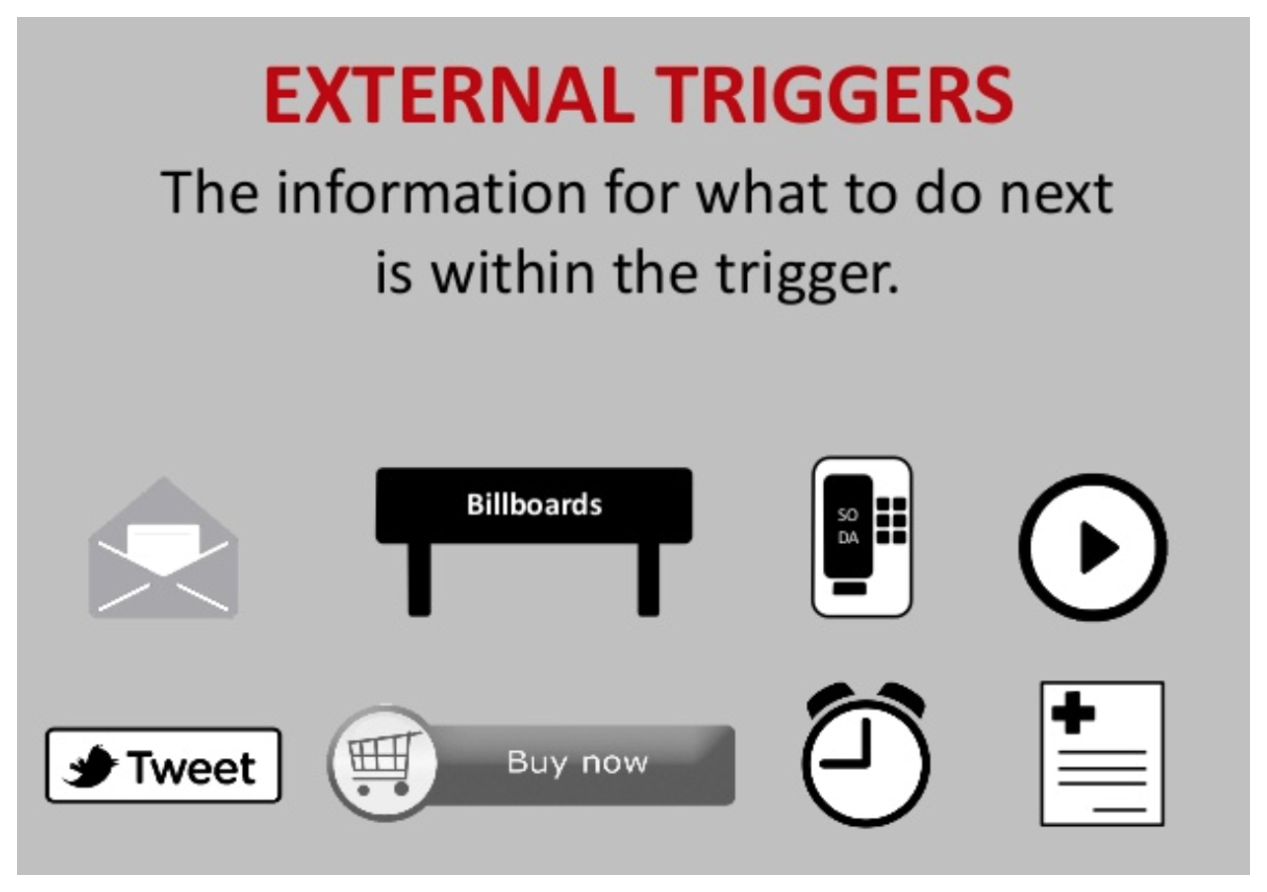
\includegraphics[scale = 0.4]{Bilder/externalTrigger.eps}
\caption{Beispiel äußerlicher Auslöser \cite{ExternalTrigger2018}.}
\label{externaltriggerBild}
\end{center}
\end{figure}
\\\\
Bei den äußerlichen Auslösern handelt es sich z.B. um verschieden Knöpfe in entweder digitaler oder mechanischer Form. Die Darstellung der Apps auf den Screens unsere Smartphones sind ebenfalls äußerliche Auslöser. Diese Auslöser erlauben es die folgende Aktivität (Video abspielen, E-mail lesen, Nachricht senden etc.) direkt zu starten. Diese Auslöser gibt es in verschiedensten Formen und sind klar verständlich und sehr intuitiv. Mit anderen Worten sie sind kinderleicht zu erkennen und zu bedienen \cite{Eyal2014}.
\\\\
Die innerlichen Auslöser beziehen sich nun mehr auf die menschliche Psychologie. Während die äußerlichen Auslöser sich durch technische Lösungen darstellen, sind die innerlichen Auslöser die aus dem inneren eines jeden Menschen kommen. Gemeint sind damit unter anderem, Emotionen, andere Menschen, spezielle Situationen, Orte oder gar Routinen (Abb.\ref{internalTriggerBild}).
\\
\begin{figure}[h!]
\begin{center}
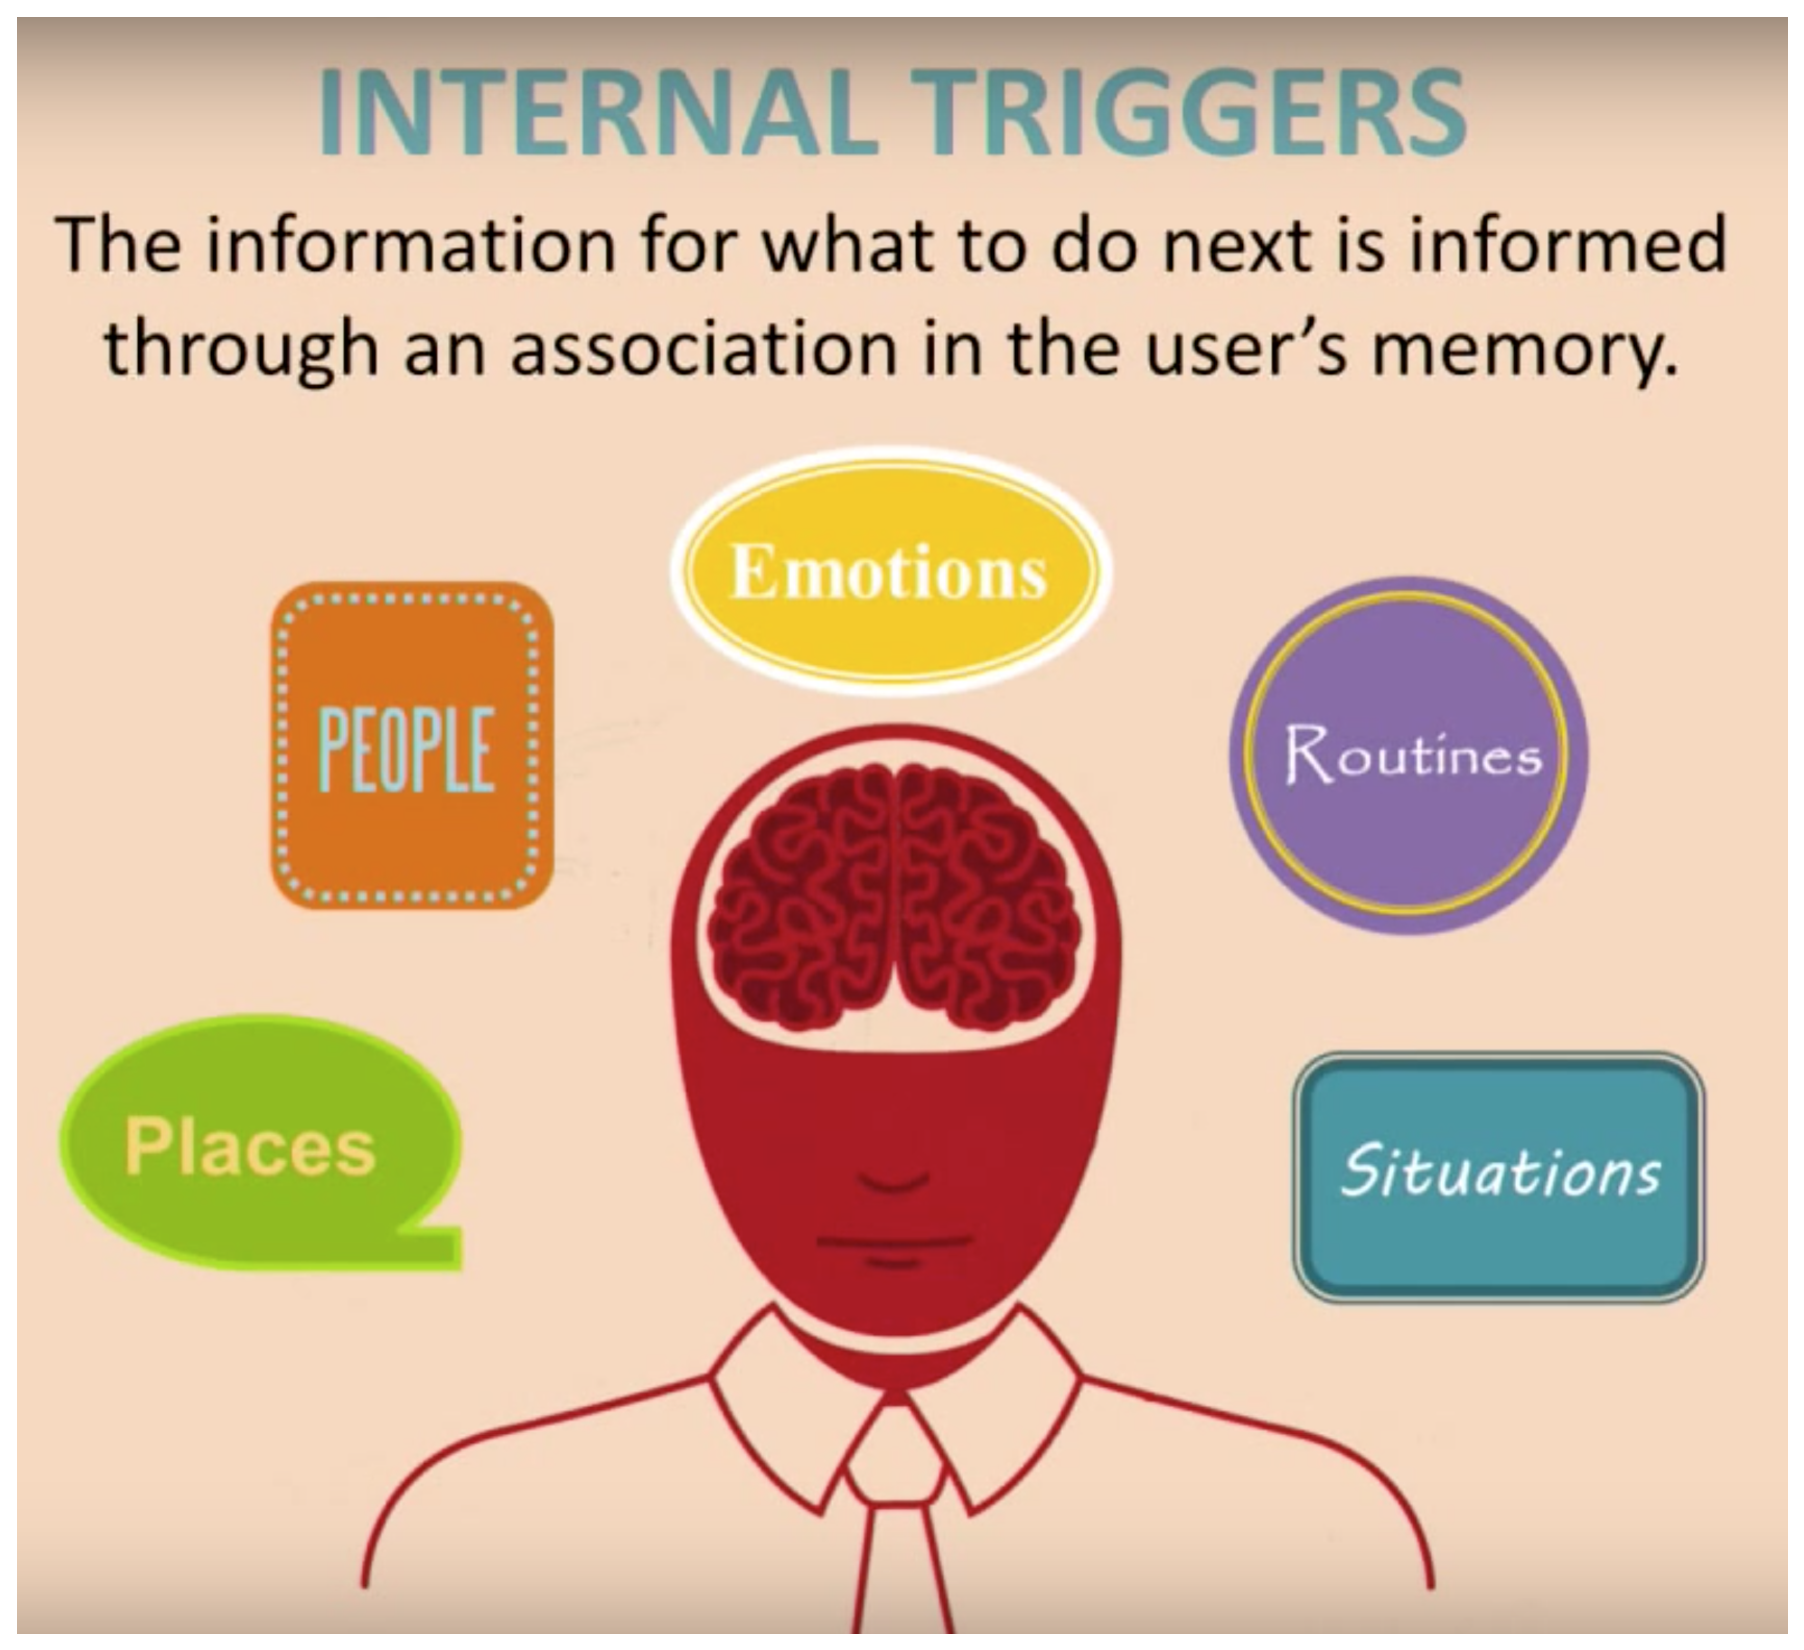
\includegraphics[scale = 0.3]{Bilder/internalTrigger.eps}
\caption{Darstellung innerlicher Auslöser\cite{ExternalTrigger2018}.}
\label{internalTriggerBild}
\end{center}
\end{figure} 
\\
Die innerlichen Auslöser werden durch die mentale Haltung (Psychologie) des Menschen verursacht. Die Information, welche Handlung auf diese Art von Auslöser folgt, wird durch eine Assoziation des entsprechenden Person und seiner Erfahrungen gezogen. Erklären wir dies an ein paar Beispielen:
\begin{enumerate}
      \item \textbf{Beispiel YouTube}: Eine Person fühlt sich gelangweilt (Langeweile als innerlicher Auslöser) also geht diese Person auf YouTube um sich ein Video anzusehen (Aktion). Durch den Auslöser wird die Person also verleitet, die Aktion durchzuführen. 
      \item \textbf{Beispiel Facebook}: Ist eine Person alleine oder fühlt sie sich alleine (innerer Auslöser), so kann sie auf Facebook gehen (Aktion) um mit Freunden oder Bekannten zu unterhalten und so dem Gefühl der Einsamkeit vorbeugen.
\end{enumerate}
Diese Beispiele lassen sich für viele soziale Media Technologien erkennen. Die Gemeinsamkeit die auch einen Teil des Erfolges dieser Technologien erklärt ist, das sie die innerlichen Auslöser der Menschen befriedigen. Viele dieser Services fangen klein an und werden über einen gewissen Zeitraum zu einer Gewohnheit des Alltages ohne die sich die meisten Menschen nicht mehr zufrieden geben würden \cite{Eyal2014}.
\\\\
Die Kombination von äußerlichen und inneren Auslösern ist nun die nächste Anforderung die aus diesem Kapitel für diese Arbeit hervorgeht. Hierbei muss sich die Gestaltung auf einfache und sehr intuitive Auslöser konzentrieren und es muss des weiteren die menschliche Seite des Dokumentationprozesses untersucht werden. Als eine generelle Idee kann der innerliche Auslöser des bekannten \enquote{AHA-Effekts} genutzt werden. Die Gestaltung der Trigger wird in den folgenden Kapiteln in Zusammenhang mit den passenden Gamification Elementen durchgenommen.  

\subsection{Zusammenfassung des Knowledge Managements}
\label{Zusammenfassung des Knowledge Managements}
Nun haben wir uns mit den Schwierigkeiten des Dokumentationsprozesses beschäftigt und haben in den Vorangegangenen Kapiteln Ansätze und Anforderungen gestellt, die an dieser Stelle nochmal zusammengefasst werden sollen.
\\\\
In diesem Kapitel haben wir den Zweck einer Wissensbasis und deren Vorteile behandelt. Wir konnten einige der Schwierigkeiten in diesem Bereich, wie z.B. das identifizieren von Informationen und die Darstellung von Informationen aufführen. Zusätzlich wurde auf die Qualitätsmerkmale eingegangen die in diesem Bereich zu finden sind. Über die Ursachen von mangelnder Dokumentation sind wir übergegangen zu Faktoren die den Prozess des Knowledge Capturing beeinflussen können. Dabei spielt das Verhaltensmodell von BJ Fogg eine wichtige Rolle. Über dieses Modell konnten konkrete Anforderungen aufgestellt werden wie der Prozess des Knowledge Capturing optimiert werden kann. Diese Anforderungen werden an dieser Stelle nochmal zusammengefasst.
\begin{description}
   \item[Anforderungsliste:]~\par
   \begin{itemize}
      \item \textbf{Motivation steigern durch Belohnung}: Wie wir gesehen haben ist der konkrete Nutzen einer Dokumentation nicht Anreiz genug um Mitarbeiter auf dauer zu motivieren. Um nun die Motivation am Dokumentationsprozess zu steigern muss eine entsprechende Belohnung für diesen Prozess entwickelt werden.
      \item \textbf{Fähigkeiten des WE-Prozesses verbessern}: Durch die verschiedenen Fähigkeitsmerkmale wie Zeit, Verständnis und soziale Abweichung muss der Prozess entschlackt und vereinfacht werden.
      \item \textbf{Auslöser finden und entwickeln}: Die entsprechenden äußerlichen und innerlichen Auslöser müssen genauer identifiziert werden. Desweiteren müssen die Auslöser entsprechend für den Dokumentationsprozess entwickelt werden.
   \end{itemize}
\end{description}
Diese Anforderungen werden in Kapitel \ref{Konzeption} nochmal aufgegriffen und für die Konzeption verwendet. Nun müssen die entsprechenden Gamification Elemente herausgearbeitet werden, mit denen sich diese Anforderungen umsetzten lassen.    
\newpage
\section{Grundlagen der Gamification}
Nach Deterding beschreibt Gamification ein Design-Konzept der HCI (Human-Computer-Interaction) \cite{Deterding2011}. Bei der Entwicklung von gamifizierten IT-Anwendungen überträgt man aus dem Game-Design bekannte Design-Elemente, Prinzipien und Mechanismen auf einen vorhandenen oder angedachten Prozess. Das Ziel ist es, Anwender bei diesem Prozess zusätzlich zu engagieren und zu motivieren. Der zu gamifizierende Prozess oder die gamifizierte Anwendung dürfen aber nicht als ein Spiel betrachtet werden, da es zwischen einem Spiel und Gamification generelle Unterscheidungsmerkmale gibt, wie beispielsweise das Fehlen von \enquote{Gameplay} sowie das Vorhanden sein einer Zweckmäßigkeit. Dies soll nochmals durch die Abbildung \ref{GamificationDiffBild} verdeutlicht werden.     
\\
\begin{figure}[h!]
\begin{center}
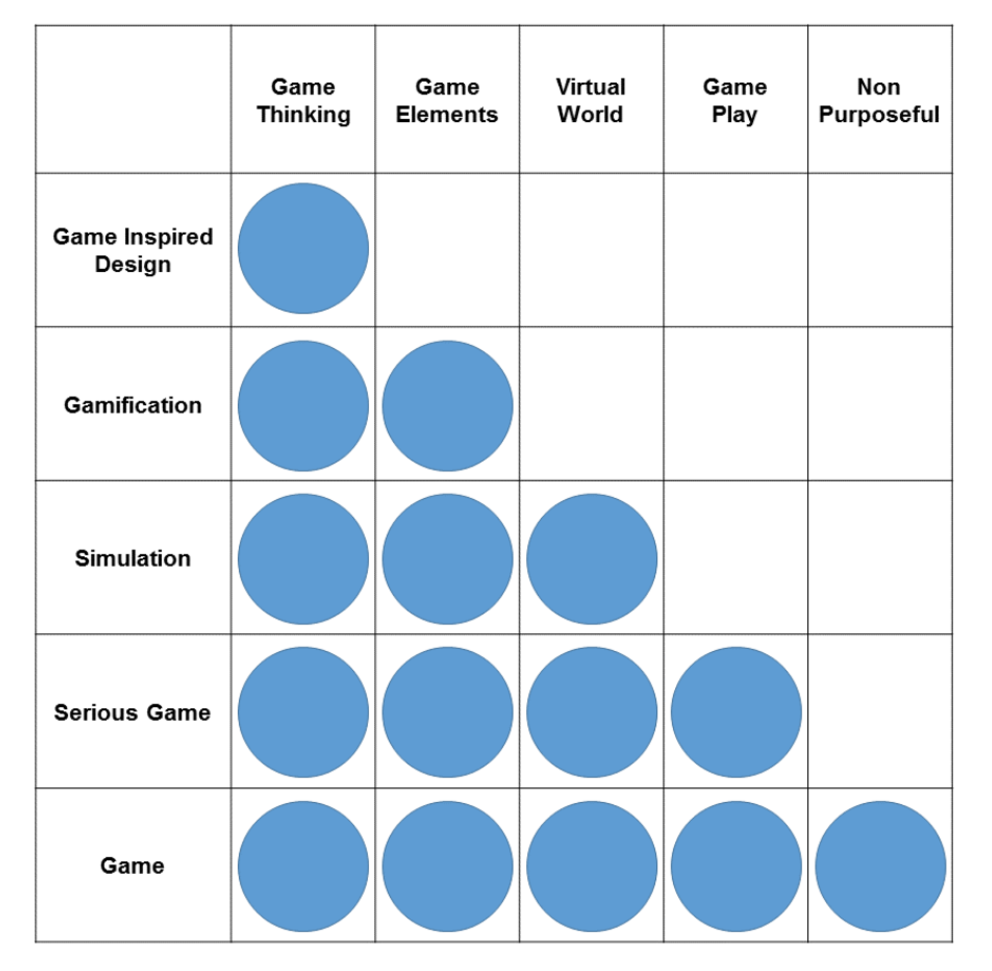
\includegraphics[scale = 0.5]{Bilder/GameVielfalt.eps}
\caption{Unterscheidung von Games und Gamification \cite{Marczewski2016}.}
\label{GamificationDiffBild}
\end{center}
\end{figure}
\\
Der gamifizierte Prozess wird also nicht zu einem Spiel, sondern erhält lediglich zusätzliche Komponenten. Dabei reicht es aber nicht aus, die Gamification Elemente einfach willkürlich an irgendwelche Schritte des Prozesses zu integrieren. Viel mehr geht es darum, den Prozess umzugestalten. Dies beinhaltet unter anderem, ihn einfacher und unkomplizierter zu designen und Elemente zu integrieren die Anwender dazu verleiten, nicht nur ihre Arbeit zu erledigen, sondern auch extra Anstrengungen in kauf zunehmen. Hierfür muss der zu gamifizierende Prozess komplett neu Überdacht werden. So muss der Prozess z.B. einem Anwender \textit{Relevanz}, \textit{Herausforderung} und \textit{Autonomie} spüren lassen. Dadurch wird aus dem Prozess eine positive Erfahrung für den Anwender, die ihn dazu verleiten kann, produktiver und effizienter zu arbeiten.
\\\\
In diesem Abschnitt sollen die Grundlagen zur Gamification geklärt werden. Zu den Grundlagen zählt der Unterschied zwischen einem Spiel und einer Gamification-Anwendung, den verschiedenen Abstraktionsebenen die aus dem Game-Design bereits bekannt sind und sich ebenfalls in der Gamification bewährt haben. Sowie den Game-Design Grundsätzen den bekannten Modellen und den verschiedenen Mechaniken. 

\subsection{Game vs. Play}
Um Gamification nicht falsch zu verstehen, ist es hilfreich zwischen \enquote{Game} und \enquote{Play} zu unterscheiden. In der englischen Sprache verwendet man \enquote{Play} für spielen, im Sinne einer spielerischen Interaktion. Diese Interaktion ist kreativ, ungezwungen bzw. frei und folgt keinen Regeln oder System. Es geht lediglich um den Spaß und um die freie Kunst sich auszudrücken, wie es Kinder in sehr jungen Jahren tun.
\\\\
Das Wort \enquote{Game} (Gaming) bezieht sich dahingegen auf Interaktionen bei denen es um Triumph oder Misserfolg geht. Diese Gaming-Interaktionen besitzen Regeln, Belohnungen, Feedback, sind Ziel orientiert und bauen auf Wettkampf auf \cite{Deterding2011}. Sie vermitteln Sieg oder Niederlage und das bewältigen oder scheitern an Herausforderungen. Sportliche Interaktionen oder Videospiele sowie Brettspiele fallen daher in den Bereich von Games und nicht in Play. 
\\\\
\enquote{\textit{There is a vast difference between games and play. Play is played for fun, but games are deadly serious and you do not play them to enjoy yourself}} \cite{Baring2014}.
\\\\
Wichtig ist diese Unterscheidung deswegen, um die Design Idee die hinter Gamification steckt zu veranschaulichen. Die Begriffe \textit{Playful}-Design und \textit{Gameful}-Design lassen sich durch die Unterscheidung zwischen Game und Play leichter näher bringen. So bezieht sich Gameful-Design (oder Game Thinking) auf den Gamification Ansatz, indem Prozesse oder Systeme mit zusätzlichen Regeln oder Mechaniken versehen werden. Diese Erweiterung kann Auswirkungen auf die Funktionalität der gamifizierten Anwendung haben. Wohingegen Playful-Design sich auf das einbringen von Gimmicks oder Spielereien beschränkt, welche nichts an der Funktionalität einer Anwendung ändern. Zwar können Playful-Design und Gameful-Design miteinander kombiniert und für Gamification genutzt werden, dennoch gibt es große Unterschiede zwischen den Beiden.
\\\\
Basierend auf dieser Einteilung (Abb.\ref{PlayGameBild}) lässt sich erkennen, dass die Gamification nicht die einzige Alternative ist, bei der die Integration von Spielaspekten im Vordergrund stehen. So gibt es neben der Gamification die \textit{Serious Games} bei denen ein komplettes Spiel vorhanden ist, dieses aber mit ernsthaften Inhalten versehen ist. Hinzukommen die sogenannten \textit{Pervasive Games} bei denen die Realität zum Spiel wird. Dabei ist zu beachten, dass all diese, und das davon herausgelöste Playful-Design, eng miteinander verwandt sind und es viele Überschneidungen gibt \cite{Deterding2011}.
\\
\begin{figure}[h!]
\begin{center}
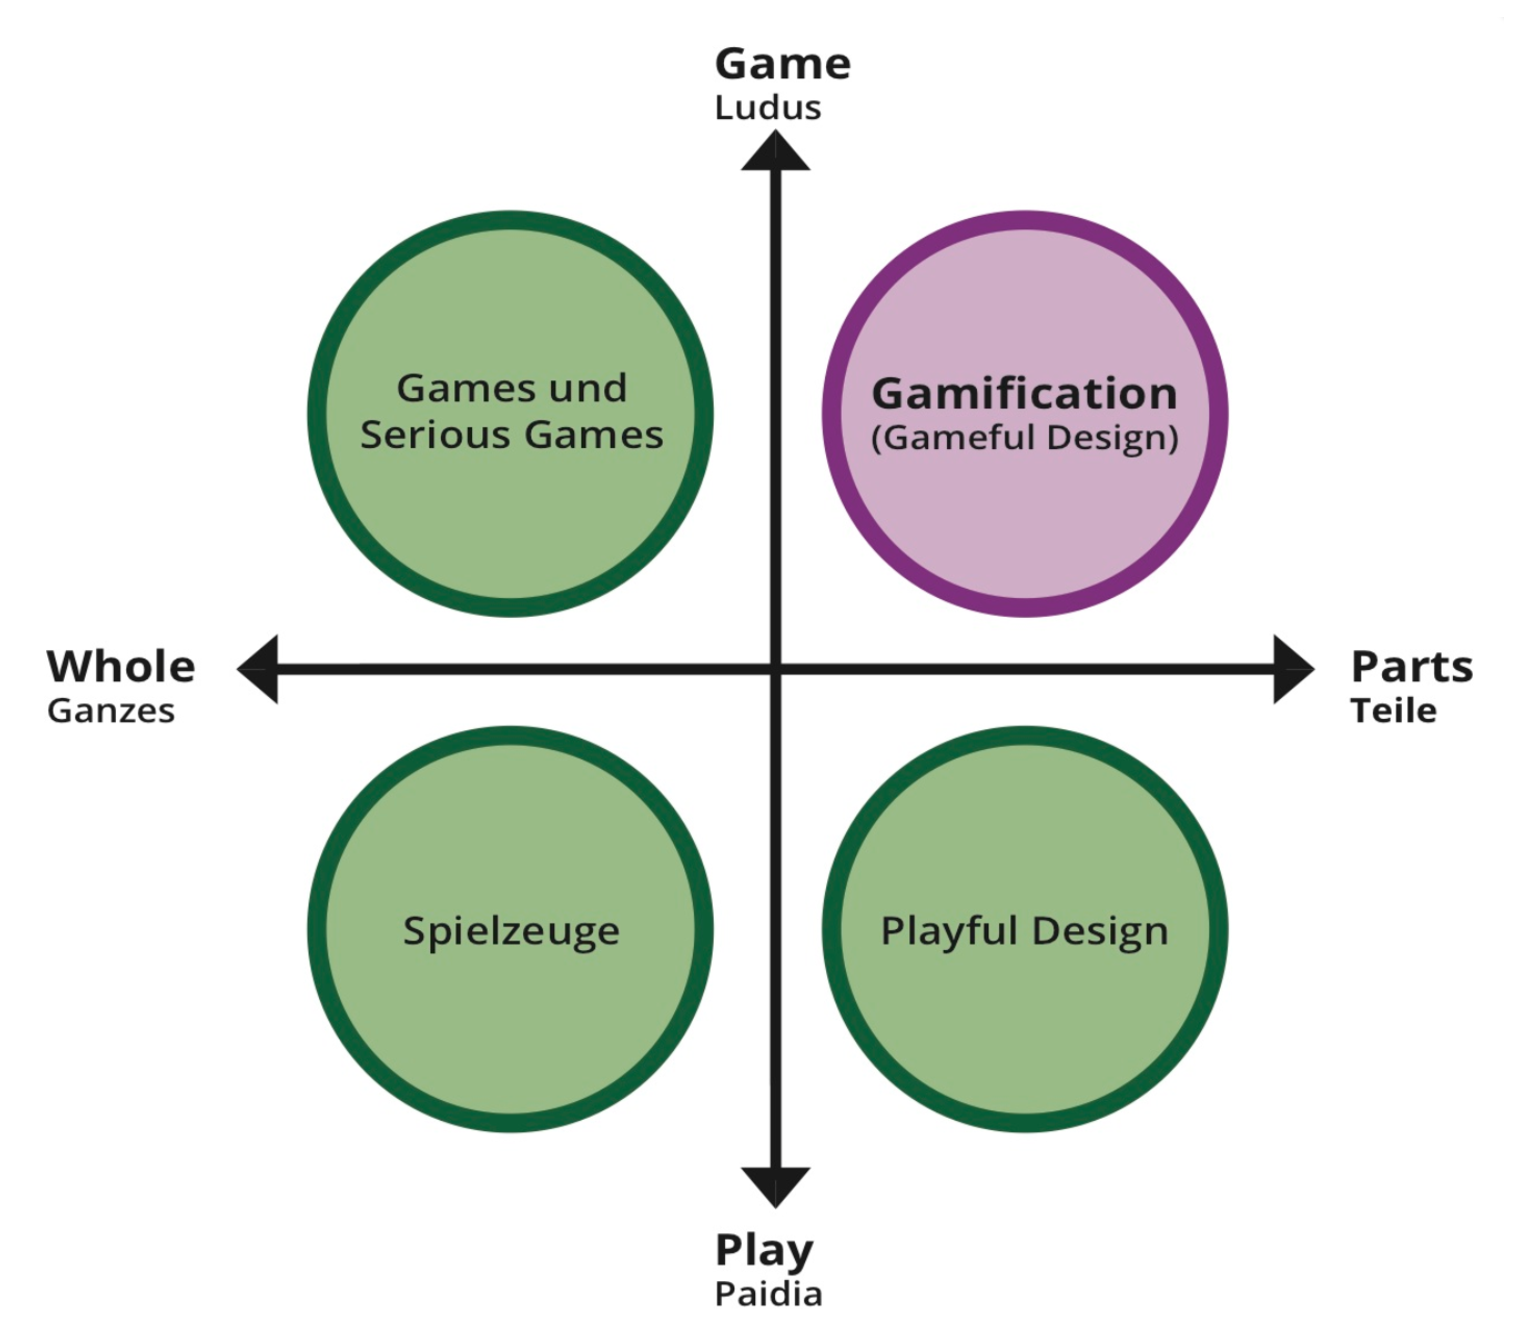
\includegraphics[scale = 0.4]{Bilder/PlayGame.eps}
\caption{Einordnung der Gamification \cite{PlayGame2018}.}
\label{PlayGameBild}
\end{center}
\end{figure}
\\
Wenn man betrachten, dass es sich bei Gamification nicht um komplette Spiele, sondern nur um das Übertragen von Game-Design Elementen handelt, so lässt sich Gamification von \textit{Serious Games}, \textit{Spielzeug} und \textit{Playful Design} abgrenzen. Diese Unterscheidung ist in Abbildung \ref{PlayGameBild} genauer zu sehen. Bei Gamification geht es somit um das Spielen im Sinne von Games und den Einsatz von Teilen aus Spielen (bzw. Spielelementen), was es von Serious Games unterscheidet \cite{PlayGame2018}.

\subsection{Game-Design Elemente}
In der Literatur zu Gamification und Game-Design finden sich zahlreiche Ansätze zur Definition von charakteristischen Elementen von Games und gamifizierten Anwendungen. Diese lassen sich in fünf verschiedene Abstraktionsebenen einteilen \cite{Deterding2011}. Die fünf Abstraktionsebenen sind in Abbildung \ref{GameElementeBild} dargestellt.
\\\\
\textbf{Abstraktionsebene 1: Interface-Elemente}\\
Auf der ersten Abstraktionsebene, welche für dem Anwender am deutlichsten wahrzunehmen ist, befinden sich die \textit{Interface-Elemente}. Diese sind meistens aus Videospielen übernommen. Zu diesen Interface-Elementen zählen unter anderem \textit{Fortschrittsbalken}, \textit{Punkte}, \textit{Abzeichen}, \textit{Ranglisten} und \textit{Level}. Diese Elemente geben den Anwender eine Rückmeldung über seinen Fortschritt, sie heben Anwender von einander ab und schaffen Wettkampf-Bedingungen. Diese Rückmeldungen sind ausschlaggebend für Gamification, da sie den Anwender auf einer tieferen Ebene ansprechen und Anwender motivieren können einer Handlung mehr Aufmerksamkeit zu schenken \cite{GameElemente2018}.
\\\\
\textbf{Abstarktionsebene 2: Game-Design Mechanismen}\\
Die zweite Abstraktionsebene enthalten die \textit{Game-Design Pattern} und \textit{Game-Design Mechanismen}. Diese bestimmen sowohl die Funktionsweise der verwendeten Interface-Elemente sowie die User Experience, welche der Anwender erlebt. Diese Mechanismen dienen dazu den Anwender anzutreiben und voranzubringen.
\\\\
\textbf{Abstarktionsebene 3: Game-Design Grundsätze}\\
Die \textit{Game-Design Grundsätze} bilden die dritte Abstraktionsebene. Hierzu zählen die psychologischen Bedürfnisse die hinter der Implementierung von erfolgreichen Gamification Anwendungen stecken. Somit enthalten die Game-Design Grundsätze die Grundlagen der Gamification. Sie gelten als grundlegenden Rahmenbedingungen für Spiele und basieren auf psychologischen Motivationsgrundlagen \cite{Werbach2012}. 
\begin{description}
   \item[Zu diesen Grundsätzen kann man diese vier Bedürfnisse zählen:]~\par
   \begin{itemize}
      \item \textbf{Kompetenz}: Umfasst das Bedürfnis, Fähigkeiten zu erlernen und Herausforderungen zu meistern. 
      \item \textbf{Autonomie}: Das Bedürfnis sich frei zu entfalten und kreativ zu sein.
      \item \textbf{Soziale Eingebundenheit}: Das Bedürfnis sich als Mitglied einer Gruppe zu fühlen.
      \item \textbf{Zweck bzw. Bedeutung}: Das Bedürfnis sich als Teil von etwas größeren zu fühlen.
   \end{itemize}
\end{description}
Diese vier Bedürfnisse werden im Kapitel \ref{Game-Design Grundsätze} noch ausführlicher behandelt.
\\\\
\textbf{Abstarktionsebene 4: Game-Design Modelle}
\\
Auf einer weiteren Ebene, der vierten Abstraktionsebene, gibt es eine Reihe von Modellen die hier als \textit{Game-Design Modelle} beschrieben werden sollen. Sie versuchen Game-Designern bei der Implementierung von Spielen zu unterstützen. Basierend auf den Game-Design Grundsätzen, lässt sich mit ihnen der erfolgreiche Einsatz der Interface-Elemente und Game-Mechaniken begründen. Es handelt sich dabei um \enquote{Conceptual models of the components of games or game experience} \cite{Deterding2011}. Diese Modelle eignen sich ebenfalls für die Implementierung von Gamification Anwendungen weswegen diese im Kapitel \ref{Game-Design Modelle} betrachtet werden.
\\\\
\textbf{Abstarktionsebene 5: Game-Design Methoden}\\
Die letzte Ebene bilden die \textit{Game-Design Methoden}. Dabei handelt es sich um Prozesse und Praktiken, welche aus der Spieleentwicklung bekannt sind und sich ebenfalls für die Implementierung von Gamification Anwendungen eignen \cite{GameElemente2018}. Bei den Methoden werden die Bedürfnisse der Anwender ermittelt, um bei der Konzeption einer gamifizierten Anwendung zu helfen. 
\\
\begin{figure}[h!]
\begin{center}
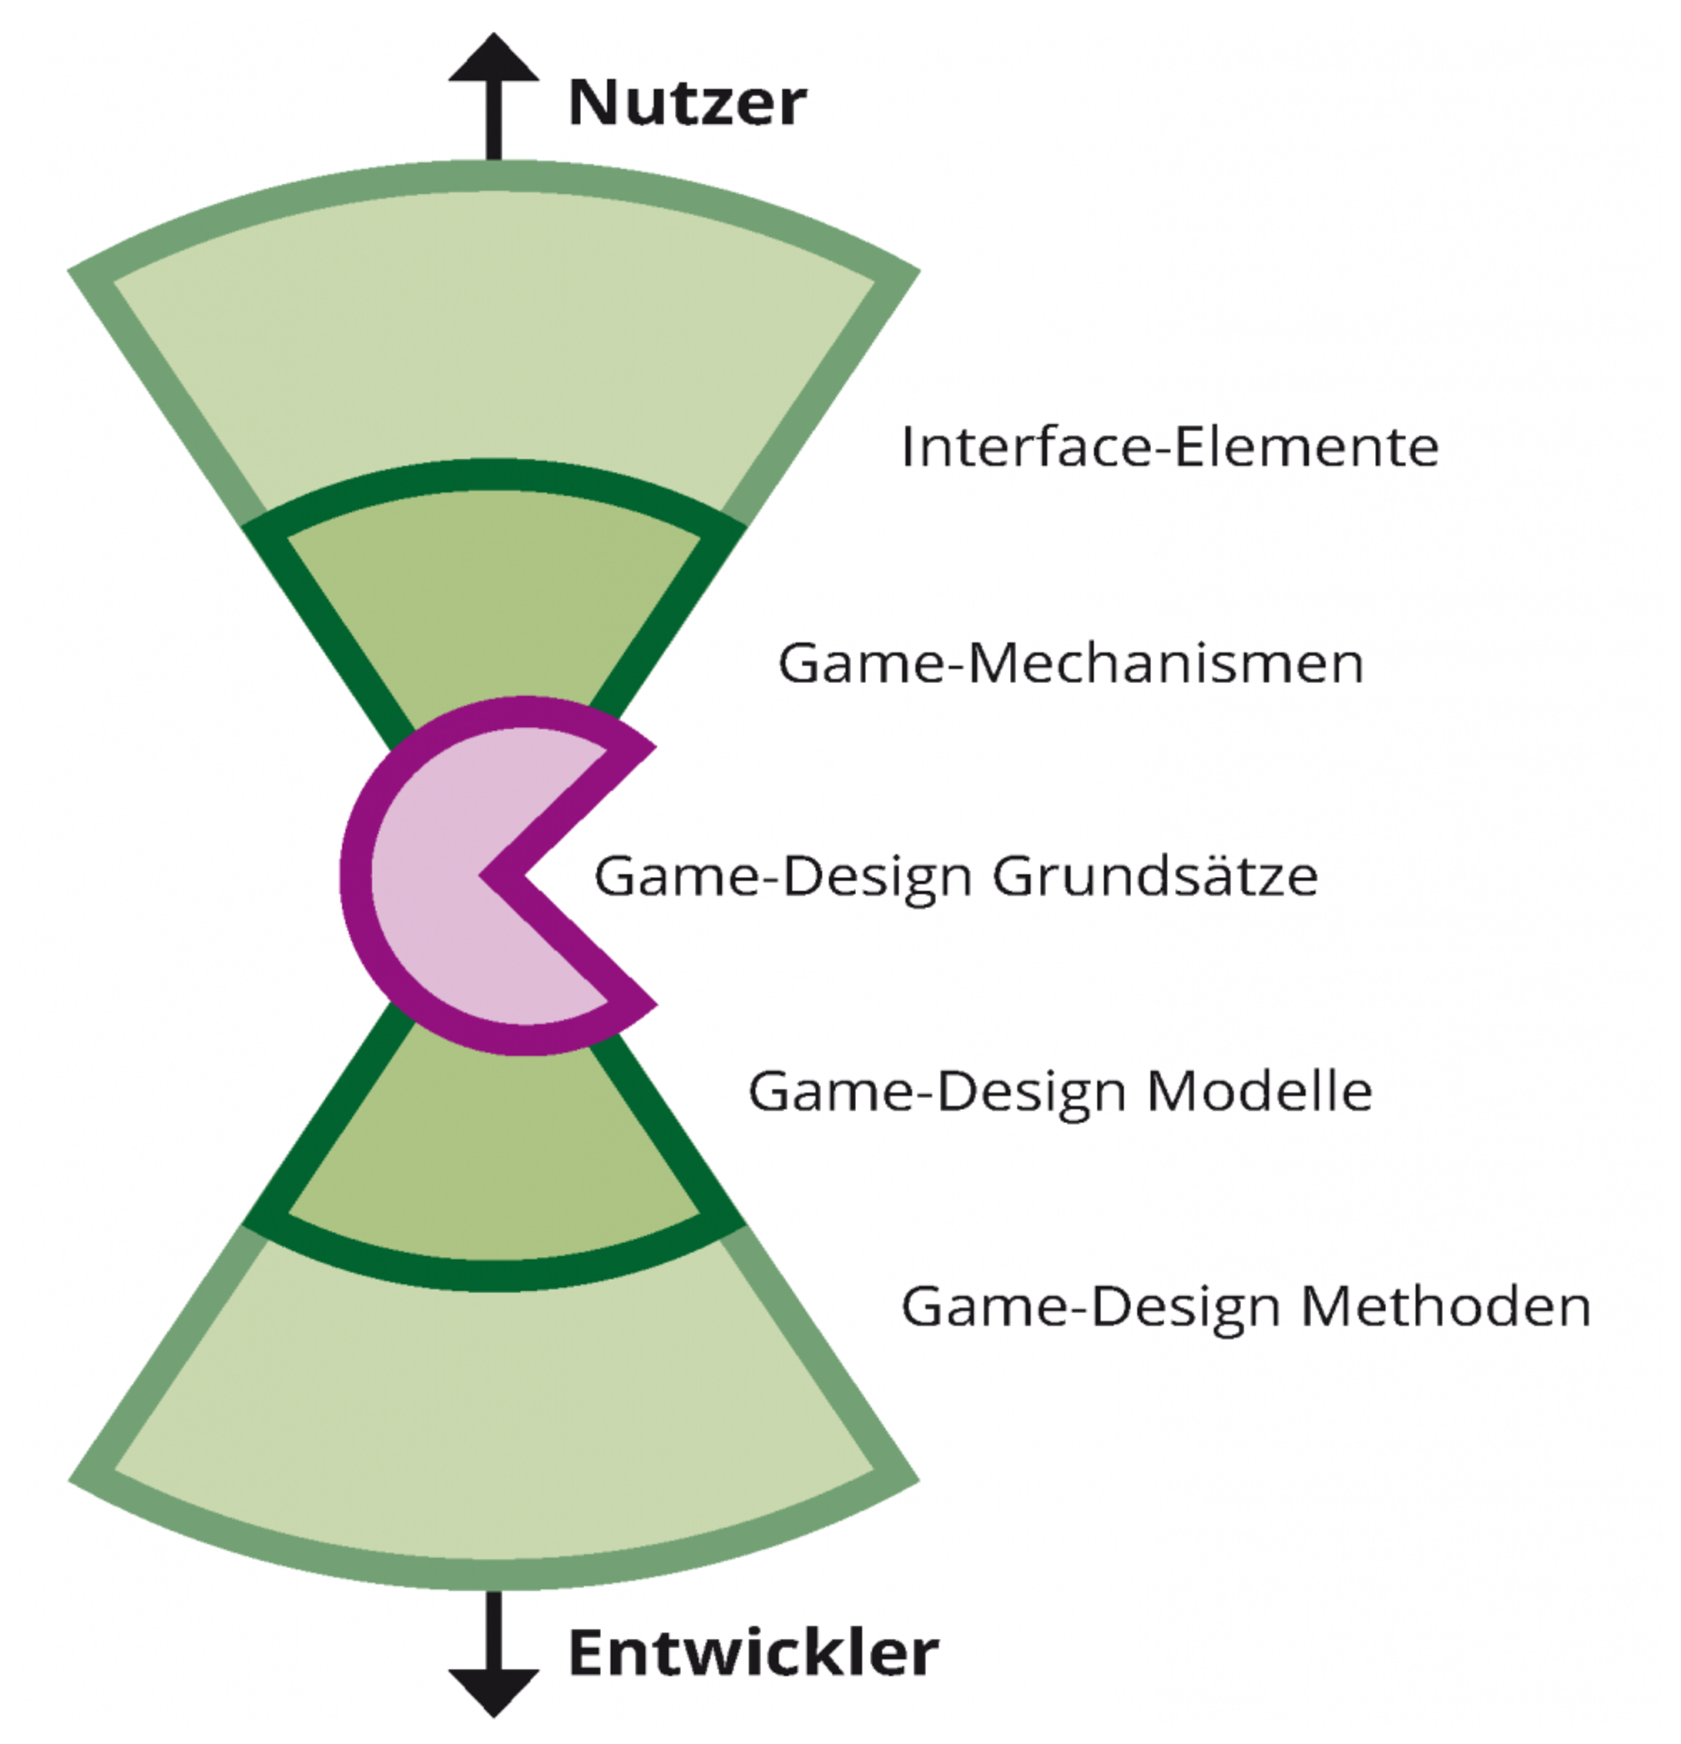
\includegraphics[scale = 0.3]{Bilder/GameElemente.eps}
\caption{Darstellung der verschiedenen Abstarktionsebenen \cite{GameElemente2018}.}
\label{GameElementeBild}
\end{center}
\end{figure}
\\
Wie in Abb.\ref{GameElementeBild} zu erkennen ist, stellen die ersten drei Ebenen die Sichtweise des Anwenders dar, während die unteren beiden Ebenen die Sichtweise des Entwicklers entsprechen. Der Kern eines soliden Game-Designs sind die Game-Design Grundsätze wie in Abb.\ref{GameElementeBild} zu erkennen ist. Die Spiele-Mechanismen und die Interface-Elemente bauen auf diesen Grundsätzen auf und geben den Anwender ein entsprechendes \textit{Erlebnis} (auch bezeichnet als Spielerlebnis, Spielerfahrung oder Player Experience). Für die Entwickler von Gamification-Anwendungen sind jedoch alle Ebenen von Bedeutung und müssen wohl durchdacht und entwickelt sein \cite{GameElemente2018}. Da die Abstraktionsebenen Aufschluss über die Umsetzung einer Gamification-Anwendung geben, ist es wichtig, diese Ebenen genauer zu betrachten. Deswegen wird auf alle Ebenen in weiteren Kapiteln eingegangen.

\subsection{Game-Design: Grundsätze}
\label{Game-Design Grundsätze}
Wie wir bereits erwähnt haben, wird Gamification verwendet um Spiele-Mechaniken und Prinzipien in nicht Spielkontexte zu übernehmen. Die Mechaniken und Prinzipien sind wiederum Elemente aus dem Umfeld des Game-Designs. Somit verwendet die Gamification also die bekannten Game-Design Elemente. Daher soll sich in diesem Kapitel mit den Grundsätzen des Game-Designs auseinander gesetzt werden.
\\\\
In ihrem Buch \enquote{Reality is broken} beschreibt Jane McGonigal (Gamification-Visionärin und Game-Designerin) die Eigenschaften eines Spiels als, \textit{Ziel}, \textit{Regeln}, \textit{Feedback-System} und \textit{freiwillige Teilnahme} \cite{Mcgonigal2011}. Diese Eigenschaften gelten auch für die Gamification und müssen beim Entwickeln einer Gamification-Anwendung berücksichtigt werden.
\begin{description}
   \item[Bedeutung der Spieleigenschaften für die Gamification:]~\par
   \begin{itemize}
      \item \textbf{Ziel}: Für die Gamification gelten zwei Ziele die übereinstimmen müssen. Nämlich die Geschäftsziele, die aussagen was mit der Anwendung erreicht werden soll (Prozessziele oder Systemziele) und die Ziele des Anwenders die für ihn von Bedeutung sind. Überschneiden sich die Geschäfts- und Anwenderziele, so zeigt die Gamification ihr optimales Potenzial \cite{gamificationDefinition}. 
      \item \textbf{Regeln}: Für die Gamification gilt, das die Regeln der Gamification-Anwendung gut überlegt werden müssen. Zum Einem muss die Anwendung verhindern, dass mit ihr gemogelt werden kann, da sich dies Negativ auf das Erlebnis des Anwenders auswirken würde. Zum Anderem dürfen die Regeln der Gamification-Anwendung den Workflow der Anwendung nicht zu stark einschränken.
      \item \textbf{Feedback-Systeme}: Diese sind für die Gamification-Anwendung von großer Bedeutung, da hier kleinere Herausforderungen zu einem Flow-Gefühl führen.
      \item \textbf{Freiwillige Teilnahme}: Die freiwillige Teilnahme für gamifizierte Anwendungen ist ein schwerer Punkt. Da es sich meistens um Geschäftsprozesse bei Gamification-Anwendungen handelt, die nicht unbedingt freiwillig umgesetzt werden können. Dennoch empfiehlt es sich, die Freiheiten des Anwenders nur soweit einzugrenzen, wie es die Regeln und der Geschäftsprozess benötigen. 
   \end{itemize}
\end{description}
Bei Gamification verfolgt man das Ziel, intrinsische Motivation zu erzeugen und zu verstärken. Eine grundlegende Theorie der intrinsischen Motivation ist die Selbstbestimmungstheorie von Deci und Ryan \cite{Ryan2000}. Nach dieser bekannten Theorie verfolgen Menschen drei grundlegende Bedürfnisse, die Bedürfnisse nach \textit{Kompetenz}, \textit{Autonomie} und \textit{sozialer Eingebundenheit} \cite{Rheinberg2006}. Nach Rigby und Ryan \cite{Rigby2011} finden sich diese drei Bedürfnisse in allen Spielen wieder. Sie sehen die Befriedigung dieser Bedürfnisse als die Grundlage eines jeden Spiels und identifizieren dies als wesentlichen Auslöser des Spielspaßes. Nach Rigby und Ryan verursachen Videospiele große Freude, da Spiele diese wesentlichen, menschlichen Bedürfnisse befriedigen \cite{Rigby2011}.

\subsubsection{Das Kompetenz-Bedürfnis}
In der Psychologie wird die \textit{Kompetenz} als das grundlegende Bedürfnis der Menschen nach Erfolg, Effizienz, Meistern von Herausforderungen und das verbessern der eigenen Fähigkeiten verstanden. Dabei geht es auch darum, die eigenen Fähigkeiten zu erfassen, zu messen und besser einschätzen zu können. Dieses Bedürfnis begleitet uns von Geburt an und führt zu starker intrinsischer Motivation \cite{Rigby2011}. Wir befriedigen dieses Bedürfnis indem wir uns Aktivitäten aussetzen die uns fordern oder indem wir uns in einem Wettkampf mit anderen Menschen vergleichen. Die Aktivitäten des Sports oder auch Videospiele erfüllen dieses Bedürfnis und so vermutet man, dass diese Aktivitäten deswegen so beliebt sind \cite{Mcgonigal2011}\cite{Rigby2011}\cite{Mayer2009}. Ein Spiel ermöglicht eine simple Bestätigung der eigenen Kompetenz.
\\\\
\enquote{\textit{Never before in human history could this kind of optimal, emotional activation be accessed so cheaply, so reliably, so quickly}} \cite{Mcgonigal2011}.
\\\\
\enquote{\textit{When games provide us with challenges, they are inviting us to stretch ourselves to new levels of mastery, which, once achieved, satisfy our intrinsic need for competence}} \cite{Rigby2011}. 
\\\\
Die \textit{Flow-Theorie} bietet eine Erklärung und eine Darstellungsweise für das Kompetenz-Bedürfnis (Abb.\ref{FlowModelBild}). Finden wir eine Lösung für ein Problem oder überwinden wir eine andere Art von Hindernis, so wird die Kompetenz erlebt \cite{Csikszentmihalyi2017}. Dabei ist eine direkte Korrelation zwischen Herausforderung und Fähigkeit wichtig um in den Flow-Zustand zu kommen. Stimmen sowohl Herausforderung (Difficulty) und Fähigkeit (Skill) überein, so bestätigt der Mensch seine eigene Kompetenz. Ist die Herausforderung zu groß, so verspüren Menschen Frust (Anxiety), ist die Herausforderung zu einfach, so verspüren Menschen Langeweile (Boredom).
\begin{figure}[h!]
\begin{center}
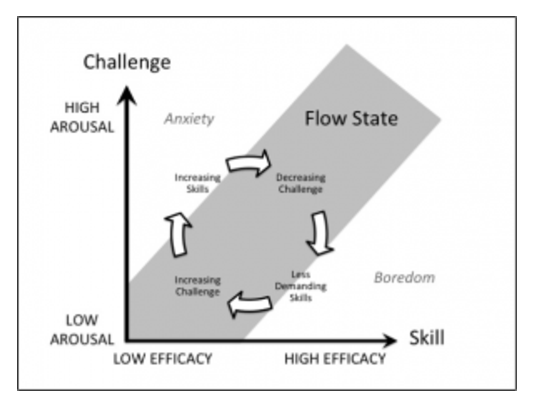
\includegraphics[scale = 0.6]{Bilder/FlowModel.eps}
\caption{Darstellung des Flow Modells \cite{FlowModel}.}
\label{FlowModelBild}
\end{center}
\end{figure}
Aus dieser Überlegung heraus ist es bei Videospielen nicht unbedingt erforderlich, grafisch auf den neuesten Stand zu sein oder über eine emotionale Geschichte zu verfügen (obwohl diese Eigenschaften helfen können). Stattdessen reicht eine Spielsteuerung, die das Kompetenz-Bedürfnis nach dem Flow-Modell befriedigt. Alte Klassiker dieses Bereichs wie \textit{Pong} oder \textit{Tetris} können hier als Beispiele erwähnt werden. Videospiele haben den Vorteil, dass sie sich einem Spieler und seinen Fähigkeiten anpassen können. Dadurch kann das Flow-Erlebnis immer wieder erfolgen und den Spieler dadurch fesseln. Wenn es also gelingt, diese Erfüllung des Kompetenz-Bedürfnis auf Geschäftsprozesse zu übertragen, so wird die intrinsische Motivation diesen Prozess durchzuführen erhöht und das Engagement mit diesem Prozess nimmt zu.
\\\\ 
\enquote{\textit{Video games […] keep us optimally challenged. […] They keep pace with our growing mastery, offering us new challenges just when we’re ready to move on from old ones}} \cite{Rigby2011}.
\\\\
\enquote{\textit{Fun is just another word for learning – Fun from games arise out of mastery. It arises out of comprehension. It is the act of solving puzzles that make games fun. With games, learning is the drug}} \cite{Koster2013}. 
\\\\
Das Spielen ist ein Lernprozess und ein Prozess stetiger Verbesserung der eigenen Fähigkeiten \cite{Rigby2011}. Stellt man sich einer Herausforderung, gibt es in der Regel nur zwei Ausgangsmöglichkeiten. Entweder man überwindet die Herausforderung und ist somit erfolgreich oder man scheitert an der Herausforderung und erleidet eine Niederlage. Kurz gesagt, entweder man gewinnt oder verliert. Sowohl Sieg als auch Niederlage sind für das erleben der Kompetenz verantwortlich. Das Scheitern ist somit ein integraler Teil des Games bzw. einer Gamification-Anwendung \cite{Mcgonigal2011}\cite{Lazzaro2004}. Ein Spiel bei dem wir immer gewinnen oder bei dem wir nicht verlieren können, löst kein Kompetenz-Erlebnis aus und wird für Menschen uninteressant. Sobald wir also ein Spiel gemeistert haben und jede Herausforderung bewältigen können, macht dieses Spiel weniger Spaß als zuvor. Aus diesem Grund ist es auch wichtig, Situationen in die Anwendung zu integrieren, die einem Anwender oder Spieler das Gefühl einer Niederlage vermitteln. 

\subsubsection{Das Autonomie-Bedürfnis}
\label{Punkte und Belohnungen}
Autonomie beschreibt das intrinsische Verlangen, sich nach eigenem Willen entfalten zu können. Dazu gehört, sich aus einer Menge von Ansätzen und Möglichkeiten frei diejenigen auszuwählen, die am Besten zu einem passen \cite{Rigby2011}. Menschen verfügen über das grundlegende Bedürfnis, sich selbstbestimmend zu erleben und wünschen sich, nach ihren eigenen Vorstellungen handeln zu dürfen bzw. zu können.
\\\\
\enquote{\textit{People are naturally motivated to seek out and stay engaged with those activities that instill a sense of personal autonomy}} \cite{Rigby2011}.
\\\\
\enquote{\textit{Researchers around the world have published hundreds of studies looking at how autonomy operates to both motivate and sustain behaviors as well as to foster feelings of well-being and satisfaction}} \cite{Rigby2011}.
\\\\
Autonomie ist neben dem Kompetenz-Bedürfnis ein weiterer Grund, weshalb das Spielen als Aktivität so fesselnd auf Menschen wirkt. Dabei gibt es bei Spielen die Möglichkeit, Autonomie auf verschiedene Arten zu spüren. So kann Autonomie erlebt werden, indem man in andere Rollen schlüpft, die Wahl hat sich zwischen mehreren Lösungswegen zu entscheiden oder das entwickeln von verschiedenen Strategien ermöglicht.
\\\\
Darüber hinaus sind Spiele kein Zwang, sie sind freiwillig und erfüllen damit schon automatisch das Autonomie-Bedürfnis. Der menschliche Wille, sich dem Spiel und seinen Regeln zu beugen steht im Zentrum. Man kann die herausfordernden Aufgaben eines Spiels annehmen, man muss aber nicht \cite{Rigby2011}. Dadurch zeigt sich die Selbstbestimmung. 
\\\\
\enquote{\textit{Playing a game is the voluntary attempt to overcome unnecessary obstacles}} \cite{Mcgonigal2011}.
\\\\
An dieser Stelle soll nun auch erwähnt werden, wie man intrinsiche Motivation schwächen kann. Der Erhalt von Belohnungen vermag ein Spiel oder auch ein Hobby, in Arbeit zu verwandeln (es muss aber nicht) \cite{Pink2010}. Dies geschieht unter anderem, wenn der Wunsch nach der Belohnung größer ist, als der Wunsch die Tätigkeit auszuführen. Wenn der Mensch sich die Belohnung als Ziel setzt und sich der Herausforderung nur der Belohnung wegen stellt, so kann der sogenannte \textit{Korrumpierungseffekt} auftreten \cite{Rheinberg2006}. Durch diesen Effekt wird beschrieben, wie extrinsische Belohnungen die Motivation des Menschen schwächen können. Man vermutet, dass der externe Anreiz einer extrinsischen Belohnung vom eigentlichen Interesse an der Tätigkeit ablenkt \cite{Rheinberg2006}. Dies führt wiederum zu einem Verlust der Motivation.   
\\\\
Studien zeigen das extrinsische Belohnungen bei Kreativen-Tätigkeiten kontraproduktiv sind und nicht zu einer Leistungssteigerung führen \cite{Pink2010}. Verspricht man aber Leuten die einer Akkord ähnlichen Arbeit nachgehen eine extrinsische Belohnung, so werden diese Leute produktiver und somit leistungsfähiger. Deswegen vermutet man, dass extrinsische Belohnungen dazu führen, dass der Fokus nun auf die Belohnung gelenkt wird, was sowohl Ablenkungen als auch kreative Ansätze mindert. Dadurch werden also Tätigkeiten denen z.B. kein kreativer Lösungsansatz voraus geht für Menschen motivierender (gemessen anhand der erhöhten Produktivität). Menschen mindern aber durch den Fokus auf die Belohnung ihre Vorstellungskraft und Kreativität, was dazu führt, dass die Produktivität dieser Tätigkeiten nicht erhöht sondern stattdessen vermindert wird.

\subsubsection{Das Eingebundenheits-Bedürfnis}
Soziale Eingebundenheit (Relatedness) beschreibt ein weiteres grundlegendes Bedürfnis, welches für intrinsischer Motivation verantwortlich ist. Dieses Bedürfnis ist von Natur aus in jedem Menschen vorhanden. Menschen suchen den Kontakt zu anderen Menschen und haben das Bedürfnis, auf sinnvolle Weise miteinander zu interagieren. Dies spielt sowohl im beruflichen Sinne eine Rolle, sowie auch im Privatleben. Beispiele für die soziale Eingebundenheit wären der eigene Freundeskreis, Mitgliedschaft in einem Verein oder Community. 
\\\\
Die soziale Eingebundenheit lässt sich in drei Teilbereiche unterteilen, die für das befriedigen dieses Bedürfnis wichtig sind. Um sich sozial eingebunden zu fühlen ist es notwendig, die \textit{Aufmerksamkeit} und die \textit{Anerkennung} anderer Menschen zu gewinnen oder sie zu spüren. Als zweiter Punkt ist die \textit{Unterstützung} von anderen Menschen von essentieller Bedeutung. Und als Letzter Punkt ist der eigene \textit{Einfluss} auf andere Menschen ein Teilbereich der sozialen Eingebundenheit. Diese drei Eigenschaften \textit{Anerkennung}, \textit{Unterstützung} und \textit{Einfluss} sind es letzten Endes, die uns ein Gefühl von starker sozialer Eingebundenheit vermitteln \cite{Rigby2011}.
\\\\
Diese drei Punkte werden in vielen \textit{Social Games} wie z.B. MMORPGs (Massive Multiplayer Online Role Playing Games) auf gewisse Art und Weise erfüllt. Natürlich ist es auch möglich, diese Social Games als Single-Player Games zu nutzen. Hierbei ist aber der Spielspaß und das Spielerlebnis eingeschränkt, was wiederum die Bedeutung der sozialen Eingebundenheit für das Social Gaming demonstriert.
\\\\
Bei sozialer Eingebundenheit geht es aber nicht nur um Teamwork. Auch Wettkampf und Wettbewerb weisen die Punkte Anerkennung, Unterstützung und Einfluss auf \cite{Rigby2011}.

\subsubsection{Das Zweck-Bedürfnis}
Der Zweck bzw. die Bedeutung (Purpose) werden zusätzlich als ein weiteres Bedürfnis der Menschen gesehen, das intrinsische Motivation hervorruft \cite{Pink2010}. Der Zweck kann als das Bedürfnis verstanden werden, unserem Handeln einem Sinn zu geben. Menschen suchen nach einem Sinn in ihrem Leben und Handeln. Sie wünschen sich das hinter ihrem Handeln eine größere Bedeutung steckt. Desto mehr Bedeutung wir unserem Handeln abgewinnen können, desto stärker werden wir intrinsisch motiviert. 
\\\\
Ein sehr bekanntes Beispiel für intrinsische Motivation die durch Bedeutung ausgelöst wird ist Wikipedia. Wikipedia verfügt nicht nur über Millionen von Artikeln sondern auch über tausende von Helfern und Autoren. Diese Menschen stellen ihr Wissen frei zu Verfügung allein aus der Überzeugung heraus, dass sie verantwortlich sind für das Archivieren und das Schützen des menschlichen Wissens. Diese Menschen schaffen ein tieferes und verbessertes Verständnis, allein aus dem Gefühl her, die Welt ein kleinwenig zu verbessern.
\\\\
Viele Menschen sprechen von Altruismus (Selbstlosigkeit), wenn sie von einem Zweck sprechen. Menschen die auf ihre eigene Art und Weise das Wohlergehen anderer über das eigene stellen. Dieser Altruismus kann eine Spende für wohltätige Zwecke sein, die Beantwortung von Fragen in einem Forum (z.B. Quora) oder das Öffnen der Tür für eine andere Person. Dieses Gefühl das von einem bedeutenden Zweck ausgeht, ist ein wichtiger Faktor für intrinsische Motivation.
\\\\
Besonders in Unternehmen ist man in der Lage, einen Zweck oder eine Berufung zu finden oder zumindest eine Grundlage dafür zu schaffen. Dafür gibt es viele Möglichkeiten. Zum Beispiel wäre ein Forum möglich, auf dem sich Mitarbeiter untereinander austauschen und sich gegenseitig Hilfestellungen geben könnten. Dies verbindet sich ebenfalls mit dem Bedürfnis der soziale Eingebundenheit, wenn man die internen sozialen Netzwerke betrachtet.
\\\\ 
Eine weitere Möglichkeit wäre, Mitarbeitern die Möglichkeit zu geben für Wohltätigkeitsorganisationen zu spenden. Insbesondere in Punktesammelplattformen ist es sehr motivierend, anstelle von Abzeichen oder Punkten, eine Hilfsorganisation zu unterstützen.

\subsection{Game-Design: Modelle}
\label{Game-Design Modelle}
Wie wir bereits erwähnt haben, dienen die Game-Design Modelle dazu, dem Entwickler bei der Konzeption eines Games oder einer Gamification-Anwendung zu unterstützen. Nach Deterding et al. \cite{Deterding2011} ist die Kombination aus Interface-Elementen und Spiele-Mechaniken (Game-Mechanics) einer der ausschlaggebende Faktoren für die Erzeugung einer ansprechenden Spielerlebnisses (Player Experience bzw. User Experience). Abhängig von Situation und Bedürfnissen der Anwender scheint es am Game-Designer zu liegen, ein erfolgreiches Gamification-Konzept zu entwickeln. 
\\\\
Aus diesem Grund sollen drei dieser Game-Design Modelle aufgezählt und näher betrachtet werden. Durch diese Analyse der Modelle soll ein besseres Verständnis dafür geschaffen werden, was beim Design einer Gamification-Anwendung zu beachten ist.

\subsubsection{Core Elements of the Gaming Experience-Modell}
Die \textit{Core Elements of the Gaming Experience} (CEGE) ist ein umfassendes Modell, das aus verschiedenen Faktoren besteht, die zusammengenommen das Erlebnis zwischen einem Videospiel (Game) und seinem Nutzer bilden (User Experience).  Die beiden wichtigsten Variablen, die dem Modell zugeordnet sind, sind \textit{Video-Game} und \textit{Puppenspiel}(Puppetry). Video-Game ist einfach das Spiel selbst, das in die latenten (subjektiven bzw. nicht messbaren) Variablen von \textit{Umgebung}(Environment) und \textit{Gameplay} aufgeteilt wird. Diese latenten Variablen werden abgeleitet und unter beobachtbaren Variablen kategorisiert; Umgebung beinhaltet \textit{Grafiken} und \textit{Sounds} des Spiels, während Gameplay das \textit{Szenario} und die \textit{Spielregeln} beinhaltet \cite{CEGE2016}.
\\\\
Puppenspiel ist die Interaktion des Spielers mit dem Videospiel und besteht aus drei latenten Variablen: \textit{Kontrolle} (Control), \textit{Eigentum} (Ownership) und \textit{Moderatoren} (Facilitators). \textit{Kontrolle} ist einfach \enquote{Kontrolle} über das Spiel, indem man lernt, wie man Dinge innerhalb des Spiels benutzt und manipuliert. Diese Kontrolle besteht aus drei beobachtbaren Faktoren: \textit{kleine Aktionen} (grundlegende Aktionen, die der Spieler im Spiel ausführen kann), \textit{Ziel} (Hauptziel des Spiels) und \textit{something-to-do} (der Spieler muss das Gefühl haben, dass es im Spiel immer etwas zu tun gibt) \cite{CEGE2016}. 
\\\\
\textit{Eigentum} (Ownership) ist, wenn der Spieler seine Aktion im Spiel als seine eigene ausführt und letztendlich durch das Spiel für diese belohnt wird. Das Eigentum setzt sich aus vier beobachtbaren Faktoren zusammen: \textit{große Aktionen} (Strategien, die vom Spieler verwendet werden, die aus vielen kleinen Aktionen bestehen), \textit{you-but-not-you} (der Spieler kann an Aktionen teilnehmen, die er nicht unbedingt im wirklichen Leben machen würde), \textit{persönliche Ziele} (etwas, das nicht wichtig ist, um das Spiel zu gewinnen, aber eine Aktion, die aus einem persönlichen Grund abgeschlossen wurde) und \textit{Belohnung} (das Spiel muss dem Spieler Belohnungen bieten)\cite{CEGE2016}. 
\\\\
Schließlich sind \textit{Moderatoren} (Facilitators) externe Faktoren, die den Interaktionsprozess zwischen einem Videospiel und dem Benutzer beeinflussen können. Diese Moderatoren bestehen aus drei beobachtbaren Faktoren: \textit{Ästhetik} (wie das Spiel für den Spieler aussieht), \textit{Zeit} (die Zeit, die der Spieler bereit ist, dem Spiel zu widmen) und \textit{frühere Erfahrung} (frühere Erfahrungen des Spielers können beeinflussen, wie viel Zeit der Spieler bereit ist in das Spiel zu investieren). Letztendlich werden die beobachtbaren Variablen in die \textit{Umbrella-Variablen} (z.B. Gameplay und Umgebung) eingeordnet, und wenn diese Umbrella-Variablen von Videospiel und Puppenspiel erfüllt sind, wird eine positive User Experience gewonnen \cite{CEGE2016}.
\\
\begin{figure}[h!]
\begin{center}
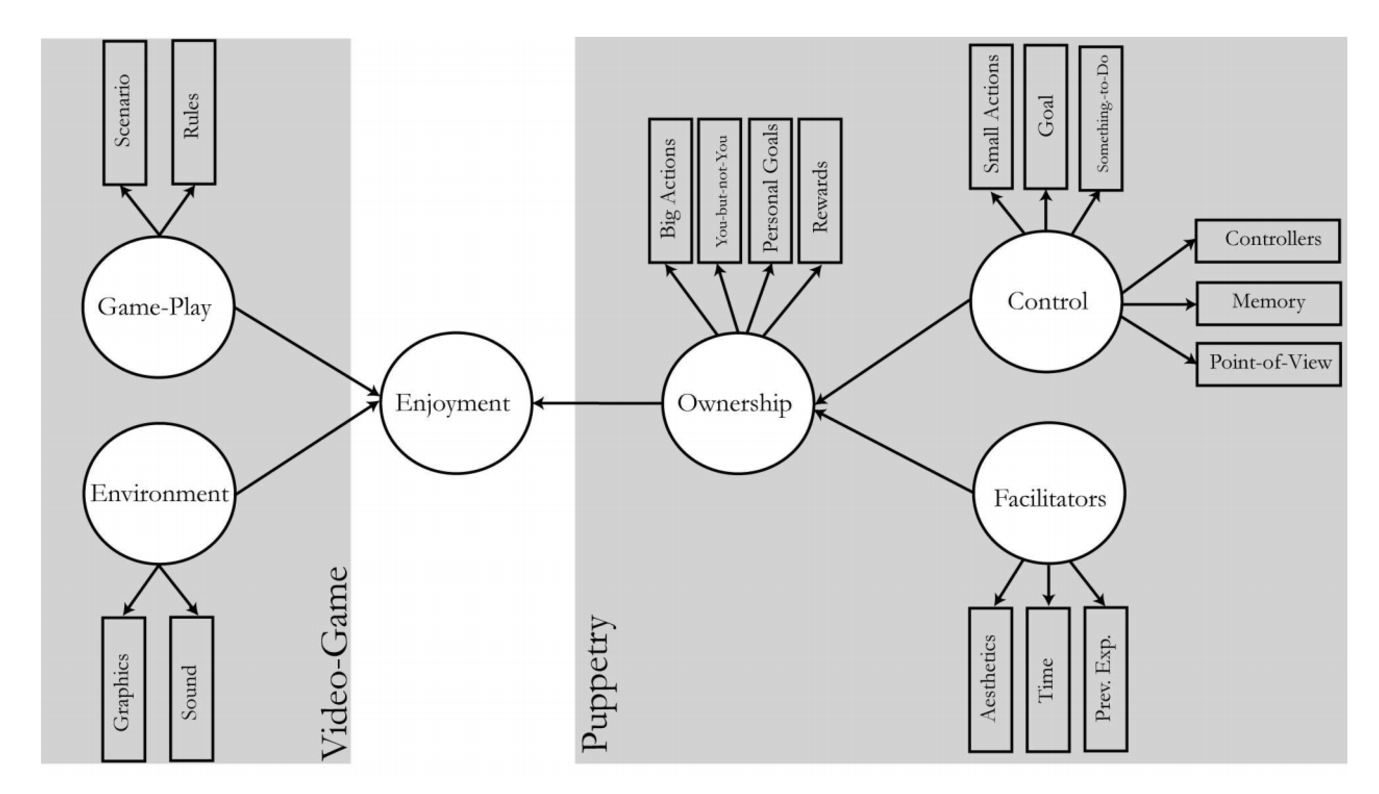
\includegraphics[scale = 0.6]{Bilder/CEGEModell.eps}
\caption{Darstellung des CEGE Modells \cite{Cege2009}.}
\label{CegeModelBild}
\end{center}
\end{figure}
\\
Die Core Elements of the Gaming Experience (CEGE) sind die Notwendigen aber nicht ausreichenden Elemente, um eine positive User Experience zu erzeugen. Dabei versucht das Modell bzw. Framework nicht zu beschreiben, was ein gutes Game ausmacht, sondern vielmehr konzentriert sich das Modell auf die Art und Weise, wie das Spielerlebnis (User Experience) wahrgenommen wird \cite{Cege2009}. 

\subsubsection{Skill Atom Modell}
Das Modell der \textit{Skill Atoms} (Fähigkeiten Atome) stammt aus den fortlaufenden
Bemühung im Spieldesign, eine Formalisierung der zentralen Bausteine von Spielen zu erreichen. Dadurch sollte eine praktisch nutzbare \enquote{Grammatik} oder \enquote{Unified Modeling Language} gebildet werden \cite{Deterding2013}. Beim Modell der Skill Atoms handelt es sich um den Versuch, die im Spiel vorhandenen Komponenten in ihre kleinsten möglichen Teile zu zerlegen (deswegen auch Atom). Die Literatur lässt vermuten, dass es sich bei Spielen (Games) um verschachtelte, mit sich selbst verbundene Systeme von Systemen handelt. Diese wiederum enthalten laut Deterding \textit{Skill Atoms}, \textit{Game Atoms} und \textit{Ludemes}. Diese drei Systeme sind die kleinsten in sich geschlossenen Systeme die nicht weiter aufgeteilt werden können, ohne ihre \enquote{Spielhaftigkeit} zu verlieren \cite{Deterding2013}.
\\\\
Ein Skill Atom beschreibt eine Feedback-Schleife zwischen einem Spieler (Player) und einem Spiel (Game), das um eine zentrale Herausforderung (Challenge) herum organisiert ist. Um die Herausforderung zu überwinden, muss der Spieler sich die dafür entsprechenden Fähigkeiten (Skills) aneignen \cite{SkillAtoms2006}.
\\\\
\enquote{\textit{A player takes an action, which forms an input into the game’s rule system, whose results gets put out as feedback to the player, which the player integrates into her understanding of the game}} \cite{Deterding2013}.
\\\\
Durch das mehrmalige durchlaufen dieser Feedback-Schleife werden dem Spieler die Fähigkeiten vermittelt, die er benötigt um das Spiel zu spielen. Ein Skill Atom besteht also aus den einzelnen Teilen: \textit{Ziel}(Goal), \textit{Aktion} (action), \textit{Token}, \textit{Feedback}, ein \textit{Regelsystem}, einer \textit{Herausforderung} (Challenge) und den \textit{Spielerverständnis} (Modell/Skill, Verständnis wie das Spiel gespielt werden will) dargestellt in Abbildung \ref{SkillAtomBild}.    
\\
\begin{figure}[h!]
\begin{center}
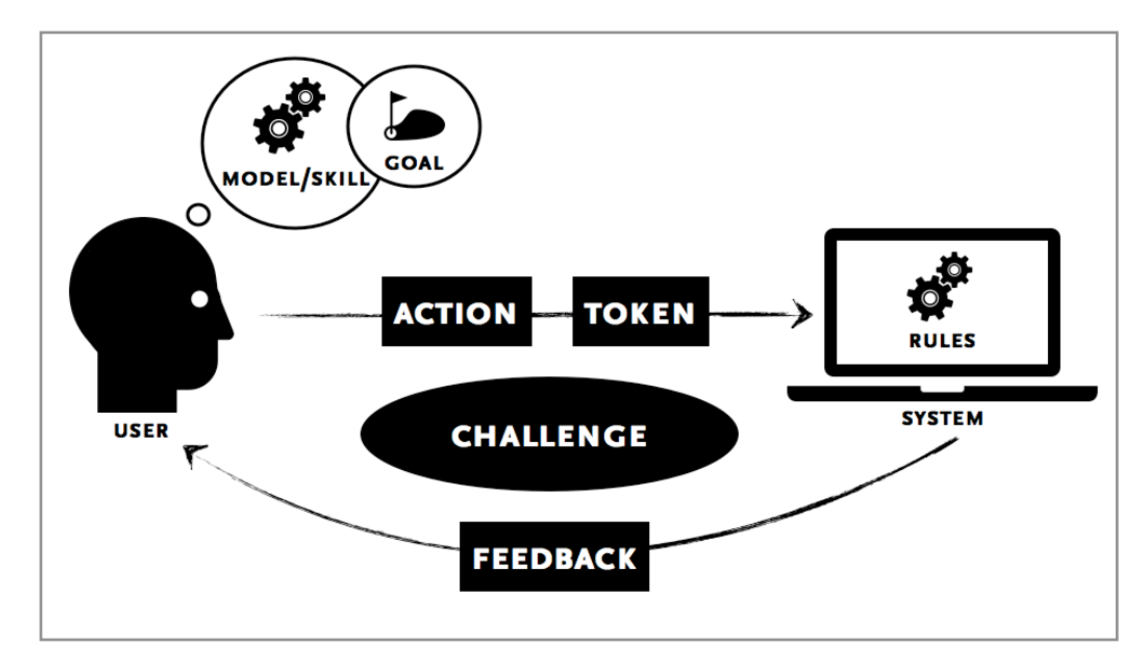
\includegraphics[scale = 0.6]{Bilder/SkillAtoms.eps}
\caption{Darstellung der Feedback Schleife, eines Skill Atoms \cite{Deterding2013}.}
\label{SkillAtomBild}
\end{center}
\end{figure}
\begin{description}
   \item[Die einzelnen Komponenten eines Skill Atoms erklärt:]~\par
   \begin{itemize}
      \item \textbf{Ziel}: Ziele artikulieren einen bestimmten Spielzustand den der Spieler erreichen will. 
      \item \textbf{Aktionen}: Was ein Spieler umsetzen kann um sein Ziel zu erreichen.
      \item \textbf{Tokens}: Einheiten auf denen der Spieler seine Aktionen ausführt.
      \item \textbf{Regeln}: Algorithmen die bestimmen, wie sich die Aktionen des Spielers auf den Spielzustand auswirken.
      \item \textbf{Feedback}: Informationen die vom Spiel an den Spieler übertragen werden, auf Antwort auf dessen handeln.	  
      \item \textbf{Herausforderung}: Die zentrale Fähigkeit (Skill), die gemeistert werden muss.
      \item \textbf{Spielerverständnis}: Das Verständnis des Spielers, wie er das Spiel zu spielen hat und seine Kapazitäten sein Spielziel zu erreichen.
   \end{itemize}
\end{description}
\subsubsection{MDA-Modell}
Das \textit{MDA-Modell} (steht für Mechanik, Dynamik und Ästhetik) ist ein formeller Ansatz um Spiele zu verstehen. Dieser Ansatz versucht, die Lücke zwischen Spieldesign und -entwicklung, Spiel Kritik und technische Spielforschung zu schließen. Das MDA-Framework formalisiert den Konsum von Spielen, indem man sie in ihre verschiedenen Komponenten zerlegt wie \textit{Regeln}, \textit{Systeme} und \textit{\enquote{Spaß}} und ihre Design-Gegenstücke etabliert, wie \textit{Mechaniken}, \textit{Dynamiken} und \textit{Ästhetik} \cite{Hunicke2004}.
\\\\
Die \textit{Mechanik} beschreibt die einzelnen Komponenten des Spiels, auf der Ebene der Datenrepräsentation und Algorithmen. Die \textit{Dynamiken} beschreiben das Laufzeitverhalten der Mechaniken, die auf die Eingaben des Spielers und gegenseitige Ausgaben im laufe der Zeit reagieren. Zum Schluss gibt es die \textit{Ästhetik} die beschreibt, wie die emotionalen Reaktionen die beim Spieler hervorgerufen werden sollen, auszusehen haben.
\\\\
Grundlegend für dieses Framework ist der Gedanke, dass Spiele eher Artefakte als Medien sind \cite{Hunicke2004}. Jede Komponente (Mechanik, Dynamik, Ästhetik) kann als seine eigene Sicht (View) auf das Spiel verstanden werden. Aus der Sicht des Designers ergeben sich aus den \textit{Mechaniken} \textit{dynamische} Systemverhalten, dieses Verhalten wiederum führt zur \textit{ästhetischer} Erfahrung. Aus der Perspektive des Spielers, wird die \textit{Ästhetik} zuerst wahrgenommen, diese besteht aus beobachtbaren \textit{Dynamiken} und ausführbaren \textit{Mechaniken} (Abb.\ref{MDAModelBild}). 
\begin{figure}[h!]
\begin{center}
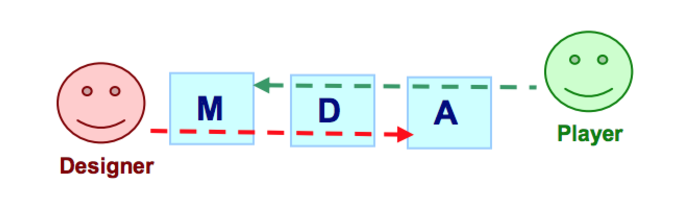
\includegraphics[scale = 1.0]{Bilder/MDAModel.eps}
\caption{Unterschiedliche Ansichten auf das MDA-Modell \cite{Hunicke2004}.}
\label{MDAModelBild}
\end{center}
\end{figure}
\\
Die \textit{Ästhetik} eines Spiels wird beim MDA-Modell in acht verschiedene Kategorien unterteilt. Diese wären \textit{Empfindung}, wie fühlt sich das Spiel an. \textit{Fantasie}, das Spiel als \enquote{Make-Believe}. \textit{Narrativ}, das Spiel als Erzählung wo die Geschichte im Vordergrund steht. \textit{Herausforderung}, das Spiel als Hindernisparcour. \textit{Kameradschaft}, das Spiel als soziales Framework. \textit{Entdeckung}, das Spiel als Innovation oder Neuland. \textit{Ausdruck}, das Spiel als Selbsterkennung. \textit{Submission}, das Spiel als purer Zeitvertreib.
\\\\
Aus diesen acht Gefühlsebenen lässt sich nun die Ästhetik eines Spieles eingruppieren. Dadurch kann man fehlende Elemente leichter identifizieren und in das Design einbringen. Ein Spiel verfügt meistens über mehr als nur eine dieser Kategorien und kann dadurch sehr flexible und frei gestaltet werden \cite{Hunicke2004}.
\\\\
Mit den \textit{Dynamiken} versucht man nun dieses ästhetische Erlebnis zu schaffen. Will man z.B. ein Spiel mit einer entsprechenden \textit{Herausforderung} versehen, so können Dynamiken wie z.B. Mehrspieler oder Rätsel eingesetzt werden. Die \textit{Kameradschaft} kann hingegen durch Spieldynamiken wie das bilden von Teams ermöglicht werden. Durch das Verknüpfen von Ästhetik und Dynamik lassen sich so Design-Fallen vermeiden.
\\\\
Als \textit{Mechaniken} können nun die verschiedenen \textit{Aktionen}, \textit{Verhalten} und \textit{Kontrollmechanismen} gesehen werden. Diese Mechaniken wirken sich nun auf die Dynamiken aus und somit auch auf die Ästhetik. So wird z.B. bei einem Karten-Spiel durch die Mechanik des Kartenmischens die Dynamik des \textit{Bluffens} ermöglicht. Durch das ineinander Greifen von Mechaniken, Dynamiken und Ästhetiken können so Konzepte einfacher entworfen werden (Abb.\ref{MDABild}). 
\begin{figure}[h!]
\begin{center}
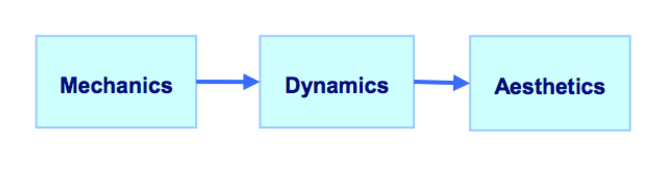
\includegraphics[scale = 1.0]{Bilder/MDA.eps}
\caption{Abhängigkeiten von Mechaniken, Dynamiken und Ästhetiken \cite{Hunicke2004}.}
\label{MDABild}
\end{center}
\end{figure}
\subsection{Game-Design Methode: Player-Centric Design}
\label{Player-Centric Methode}
Die Game-Design Methode bricht die Schritte zum entwickeln einer gamifizierten Anwendung auf und ordnet diese in logischer Reihenfolge. Die Methodik hilft den Entwicklern, sich beim Design auf das erreichen von Anwenderzielen (Anwender können auch als Spieler der Anwendung gesehen werden) zu konzentrieren und reduzieren sowohl Zeit als auch Risiken beim entwickeln einer solchen Anwendung \cite{gamificationDefinition}.
\\\\
Die \textit{Player-Centric Design} Methode gibt den Entwickler nun ein Werkzeug an die Hand, um ihn beim Design der \textit{Player Experience} (Spielererlebnis) zu unterstützen und mögliche Design-Fallen zu vermeiden. Die Player Experience soll in diesem Zusammenhang als primäres Ziel des Design-Prozesses verstanden werden. Es geht in erster Linie darum, eine Erfahrung oder ein Erlebnis für den Anwender bzw. Spieler zu entwickeln. Erfahrungen sind jedoch schwierig zu designen da es sich bei ihnen um persönliche Auseinandersetzungen handelt die über einen längeren Zeitraum auftreten. Unsere Erfahrungen wirken sich dabei stark auf unsere Wahrnehmung, auf unsere Art Wissen zu verarbeiten und auf unser Handeln aus \cite{gamificationDefinition}.
\\\\ 
Im Buch \enquote{Gamify} von Brian Burke wird beschrieben, dass die Player Experience als eine \textit{Reise} (Player Journey) zu verstehen ist. Diese Player Journey findet dabei in einem Spielraum (Play Space) statt, welche sich sowohl in der realen- als auch in der virtuellen Welt befinden kann \cite{gamificationDefinition}. Burke unterscheidet dabei auch zwischen technischen Design, das zwar wichtig ist, aber bei Player-Centric Design nicht im Mittelpunkt steht und dem Experience Design, also dem gezielten entwickeln eines Erlebnisses. Das Experience Design unterscheidet sich von herkömmlichen Software Design Methodiken, da laut Burke andere Fähigkeiten für den Experience Design Prozess benötigt werden. Zu diesen zählen unter anderem das \textit{Design Thinking}, \textit{Verhaltenswissenschaften} und \textit{emergente Systeme} \cite{gamificationDefinition}.
\\\\
Was für Gamification-Anwendungen benötigt wird ist ein Entdeckungsprozess \cite{gamificationDefinition}. Hierbei gilt es die zugrundeliegenden und manchmal versteckten Bedürfnisse der Anwender zu erkennen, um diese als Grundlage für einen Lösungsansatzes zu nutzen. Hierfür kann \textit{Design Thinking} genutzt werden. Design Thinking ist ein menschenzentrierter Ansatz (Human-centered Approach) der die Bedürfnisse des Anwenders in den Mittelpunkt des Design-Prozesses stellt. Design Thinking stützt sich auf menschliche Fähigkeiten wie \textit{Intuition}, \textit{Mustererkennung}, \textit{das konstruieren von Ideen die sowohl emotional bedeutend, als auch funktional sind} und unsere Gabe uns \textit{jenseits von Worten oder Symbolen auszudrücken}. Aus diesen Gründen eignet sich Design Thinking hervorragend für die Entwicklung von gamifizierten Lösungen.
\\\\
Der \textit{Player Experience Design Prozess} kann in sieben Schritte eingeteilt werden. Diese Prozessschritte sollen nun dem Entwicklern von Spielen oder gamifizierten Anwendungen eine Möglichkeit bieten, dass Erlebnis für den Anwender zu entwickeln.
\begin{description}
   \item[Schritte des Player Experience Design Prozess:]~\par
   \begin{enumerate}
      \item Geschäftsergebnisse und Erfolgsmetriken identifizieren.
      \item Zielgruppe bestimmen.
      \item Spielerziele bestimmen, auswählen oder entwickeln.
      \item Engagement Modell bilden.
      \item Spielraum und Reise definieren.
      \item Spiel Ökonomie gestalten.
      \item Testen und Iteration.
   \end{enumerate}
\end{description}

\subsection{Game-Design: Spiele-Mechaniken}
Die Spiele-Mechaniken (Game-Mechaniken) sind die aus Spielen bekannten Aktionen die eine Reaktion des Systems auslösen.  Sie bilden die zweite Abstraktionsebene der Game-Design Elemente und tragen mit den Interface-Elementen sowohl zur Dynamik als auch zur Ästhetik der gamifizierten Anwendung bei. Game-Designer Daniel Cook beschreibt sie als:
\\\\
\enquote{\textit{Game mechanics are rule based systems / simulations that facilitate and encourage a user to explore and learn the properties of their possibility space through the use of feedback mechanisms}} \cite{GameMechanics2006}. 
\\\\
Die Game-Mechaniken können dabei auf verschiedenen Ebenen auftreten. Auf der untersten Ebene, beschreiben sie anhand mathematischer Modelle, wie sie in der ökonomischen Spieltheorie bekannt sind, die grundlegenden Prinzipien eines Spiels \cite{Schell2014}. Auf einer höheren Ebene beschreiben sie komplexe Tätigkeiten und Herausforderungen der Spieler in einem Spiel.
\\\\
Zichermann und Cunningham \cite{Zichermann2011} haben zwölf, nach ihrer Ansicht, wesentliche Mechanismen von Reiss \cite{Reiss2009}, Schell \cite{Schell2014} und weiteren Quellen extrahiert, die sich ihrer Meinung besonders gut für das Übertragen auf Nicht-Spielsituationen eignen. Da diese einen kurzen, aber dennoch sehr guten Überblick geben, wurden sie in der folgenden Aufzählung aufgeführt. Es ist anzumerken, dass sich in all diesen Mechanismen Möglichkeiten finden lassen, mindestens eines der Grundbedürfnisse nach Kompetenz, Autonomie, sozialer Eingebundenheit und Zweck zu befriedigen.     
\begin{description}
   \item[Aufzählung der zwölf Spiele-Mechanismen nach \cite{Zichermann2011}:]~\par
   \begin{enumerate}
      \item \textbf{Mustererkennung:} Suchen und erkennen von Mustern und Strategien in einem komplexen Sachverhalt und das lösen von Rätseln. Kann als Herausforderung dienen.
      \item \textbf{Sammeln:} Sammeln von Gegenständen, Auszeichnungen, Wissen um daraus etwas zu lernen, als Satussymbol, zum Handeln, zur Erinnerung, wegen der Seltenheit. Hier wird der evolutionäre Sammeltrieb der Menschen angesprochen.
      \item \textbf{Überraschung und unerwartetes erfreuen:} Unerwartete Überraschungen, Gewinne und Auszeichnungen. Es können auch ungewohnte Objekte an ungewohnten Orten sein oder unerwartete Zusammenhänge zwischen Objekten bestehen. Durchbricht Monotonie und erzeugt spontane Freude. 
      \item \textbf{Organisieren und Ordnung schaffen:} Viele Menschen mögen es etwas zu ordnen, eigene Strukturen zu entwerfen und sich über das Ergebnis zu freuen. Hierzu gehört Ordnen unter Zeitdruck, Ordnen nach optimaler Strategie bzw. nach einem Muster oder ordnen nach Symmetrie.
      \item \textbf{Schenken:} Geschenke als Zeichen der Verbundenheit haben besonders in sozialen Netzwerken Bedeutung. Geschenke können Spieler zurück ins Spiel bringen, wenn sie länger nicht mehr aktiv waren. Zu beachten ist, dass Schenken in den verschiedenen Kulturen unterschiedliche Ausprägungen hat.
      \item \textbf{Flirten und Romanzen:} Die Möglichkeit Small Talk mit anderen zu treiben und in einem gewissen Abstand zu flirten. Viele Onlinespiele und Communities profitieren davon, dass man neue Leute kennen lernen und auf sicherer Distanz flirten kann.
      \item \textbf{Anerkennung für Leistungen:} Der am häufigsten eingesetzte Gamification Mechanismus. Dieser Mechanismus spricht generell alle Spielertypen an, insbesondere aber den Spielertyp \textit{Achiever}. Speziell im sozialen Kontext sind öffentliche Erfolge (Achievements) für Spieler erstrebenswert um sich zu profilieren.
      \item \textbf{Führen von Anderen:} Gruppen organisieren und andere anleiten. Einsatz in Team- und Kooperations-Spielen, bei denen man gemeinsam handeln muss, um ein Ziel zu erreichen. Außerdem können schwierige Aufgaben auch so ausgelegt werden, dass sie nur in Zusammenarbeit bewältigt werden können. Dieser Mechanismus kann sich unterschiedlich (positiv oder negativ) auf die Spieler auswirken.  
      \item \textbf{Ruhm und Aufmerksamkeit:} Das Präsentieren von eigenen Erfolgen bzw. des eigenen Fortschritts gegenüber anderen. Die empfundene Berühmtheit hängt von der Anzahl von Fans oder Followers bzw. Befürwortern ab. Dieser Mechanismus befriedigt das Bedürfnis der sozialen Eingebundenheit und der Kompetenz.
      \item \textbf{\enquote{Sei der Held}:} Einen Helden zu spielen bedeutet, dass man in eine besondere Rolle schlüpft. Speziell beim Helden geht es darum, eine Reihe von risikoreichen Herausforderungen zu meistern um ein Ziel zu erreichen. Heroismus kann stellvertretend für Altruismus (Selbstlosigkeit) stehen und kann zu sozialen Engagement führen. Bei diesem Mechanismus werden dem Spieler sinnvolle Tätigkeiten und bedeutende Entscheidungen zur Verfügung gestellt. Dadurch wird auch das Zweck-Bedürfnis befriedigt. 
      \item \textbf{Status und Ansehen:} Das Erringen eines Status, um zu verstehen wie wir selbst zu anderen und der Umwelt stehen. Kann in einzelnen Szenarien funktionieren, ist aber effektiver in wettbewerbsorientierten, öffentlichen Umgebungen. Der Mechanismus setzt auf Badges (Auszeichnungen), Trophäen, Levels, seltene und limitierte Gegenstände sowie eingeschränkten Zugriff auf Optionen.
      \item \textbf{Aufziehen bzw. Pflegen:} Das Aufziehen oder pflegen eines Objektes kann auf verschiedene Arten erfolgen. Das Pflegen eines Unternehmens oder einer Stadt, eines virtuellen Tiers, ein Team von Mitarbeitern die beschäftigt, diszipliniert und geleitet werden müssen. Kann sehr hilfreich sein um wiederkehrende Besuche auf einer Online-Plattform zu erhalten.
   \end{enumerate}
\end{description}
Diese zwölf Mechanismen sind natürlich nicht die einzigen die es gibt. Diese Aufzählung soll lediglich der Orientierung dienen und soll verdeutlichen, worauf es bei den verschiedenen Game-Mechanismen ankommt. Diese Auflistung zeigt sehr deutlich wie Spiele durch die verschiedenen Mechanismen zur Befriedigung unserer Bedürfnisse führen. Der Erfolg von Spielen kann also daraus geschlossen werden, dass die Mechanismen uns herausfordernde Aufgaben geben \cite{Mcgonigal2011}. Persönlicher Erfolg bei einer schweren Aufgabe führt zu starken positiven Emotionen durch biochemische Prozesse in unserem Gehirn und machen uns glücklich.
\\\\
\enquote{\textit{Fulfilling our need for better hard work-and helping us choose for ourselves the right work at the right time}} \cite{Mcgonigal2011}. 
\\\\
Wie bereits erwähnt, beruht der langfristige Spielspaß an der Erfüllung dieser Aufgaben und auf dem Prinzip der Flow-Theorie \cite{Csikszentmihalyi2017}. Ein Spiel bzw. eine Gamification-Anwendung, welche eine gute Balance zwischen Schwierigkeit und Fähigkeiten schafft, kann starke intrinsische Motivation bewirken. Die Bewältigung dieser Aufgaben, gibt uns das Gefühl, kompetent und erfolgreich zu sein \cite{Mcgonigal2011}\cite{Mayer2009}.
\\\\
Für die Gamification gilt jedoch, dass Game-Mechaniken nicht nur anhand ihrer Bedürfnisbefriedigung gewählt werden können, wie das bei Spielen der Fall ist. Bei Gamification müssen zusätzlich noch die Mechaniken auf den jeweiligen Kontext der Anwendung abgestimmt werden.  
\\\\
Neben der Motivation, die in verschiedene Gruppen eingeteilt werden kann, wie intrinsische Motivation und extrinsische Motivation, sowie den Grundbedürfnissen Kompetenz, Autonomie, soziale Eingebundenheit und Zweck, definiert Reiss vierzehn weitere \textit{grundlegende menschliche Motive} in einem Modell. Diese grundlegenden Motive hat Reiss aus mehreren wissenschaftlichen Studien zusammengetragen \cite{Reiss2009}. Diese Motive sollen an dieser Stelle ebenfalls eingehender betrachtet werden da die Mechanismen sich aus diesen Motiven ableiten lassen können.
\begin{description}
   \item[Grundlegende Motive nach \cite{Reiss2009}:]~\par
   \begin{enumerate}
      \item \textbf{Macht:} Bedürfnis danach, andere dem eigenen Willen zu unterwerfen.
      \item \textbf{Neugier:} Bedürfnis nach Kognition.
      \item \textbf{Unabhängigkeit:} Bedürfnis nach Autarkie.
      \item \textbf{Ordnung:} Bedürfnis nach Struktur.
      \item \textbf{Sparen:} Bedürfnis danach,[…] Güter zu sammeln.
      \item \textbf{Ehre:} Bedürfnis danach, sich moralisch integer zu verhalten.
      \item \textbf{Idealismus:} Bedürfnis nach sozialer Gerechtigkeit.
      \item \textbf{Beziehung:} Bedürfnis nach Freundschaft.
      \item \textbf{Familie:} Bedürfnis danach, Kinder großzuziehen.
      \item \textbf{Rache:} Bedürnis danach, mit jemand abzurechnen.
      \item \textbf{Eros:} Bedürfnis nach Sexualität.
      \item \textbf{Körperliche Aktivität:} Bedürfnis danach, seine Muskeln zu bewegen.
      \item \textbf{Ruhe:} Bedürfnis nach innerem Frieden.
      \item \textbf{Essen:} Bedürfnis nach Nahrung.
   \end{enumerate}
\end{description}

\subsection{Game-Design: Interface-Elemente}
Der Game-Charakter in gamifizierten Anwendungen wird einem Anwender als erstes durch die \textit{Interface-Elemente} bewusst. Interface-Elemente unterliegen und dienen einer oder mehreren Game-Mechaniken. Die Elemente werden als Feedback-System genutzt und haben die Aufgabe Emotionen beim Anwender auszulösen. Dadurch sind die Interface-Elemente für die Aufrechterhaltung der Motivation verantwortlich \cite{Mcgonigal2011}. Die Elemente bilden eine Wand zwischen Anwender und Anwendung \cite{Schell2014} und sollten daher einige Nutzungsbedingungen erfüllen. So sollten die Elemente nutzungsorientiert (Usability), umfangreich, leicht verständlich und zielgerichtet eingesetzt werden \cite{Schell2014}. Des weiteren sollten die Elemente über eine angemessene Ästhetik und über einen entsprechenden Reiz verfügen. Sie geben einem Anwender Feedback in Form von \textit{Beurteilungen}, \textit{Belohnungen}, \textit{Instruktionen}, \textit{Ermutigungen} und \textit{Herausforderungen}. Sie sind entscheidend für das empfinden des Anwenders und die Wirkungsweise der Game-Mechaniken. Da die Interface-Elemente viele Berührungspunkte mit dem Anwender aufweisen, müssen die Elemente gut durchdacht und ihre Wirkung umfangreich getestet werden \cite{Schell2014}.
\\\\
Die Interface-Elemente sowie die Game-Mechaniken können, da sie als Komponenten zu sehen sind, auf verschiedene Weise kombiniert und integriert werden. Dadurch sind die Elemente flexibel und vielseitig. In diesem Abschnitt sollen nun die am häufigsten auftretenden Interface-Elemente aufgezählt und ihre Funktionsweise erläutert werden. 

\subsubsection{Punkte und virtuelle Währung}
\textit{Punkte} oder eine andere Form von \textit{virtueller Währung} sind ein häufig eingesetztes Element bei Gamification-Anwendungen da sie leicht umzusetzen sind und bei richtiger Verwendung sehr mächtig sein können. Dabei werden an den Anwender Punkte vergeben, wenn dieser eine vordefinierte Handlung des gamifizierten Systems getätigt hat. Die Punkte sind dabei meistens das Eigentum eines spezifischen Anwenders, können aber auch in anderen Kontexten, als Eigentum einer Gruppe von Anwendern oder einer Community realisiert werden. Punkte dienen aber nicht als Belohnung sondern geben viel mehr Feedback über die Handlung des Anwenders und verfolgen gleich mehrere Ziele.
\\
\begin{figure}[h!]
\begin{center}
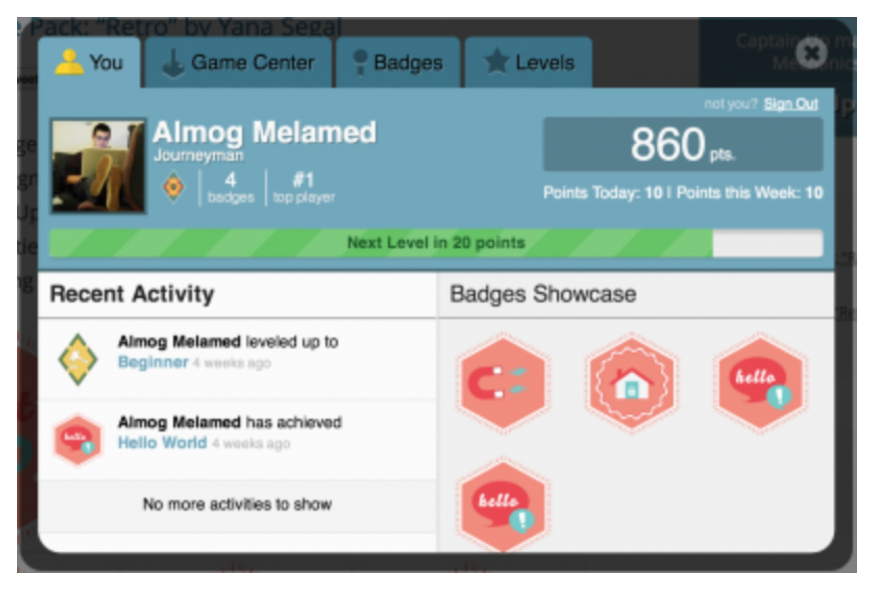
\includegraphics[scale = 0.7]{Bilder/Points.eps}
\caption{Mögliche Darstellung von Punkten \cite{Points}.}
\label{PointsBild}
\end{center}
\end{figure} 
\\
Das erste Ziel dient dem Übermitteln von Feedback an den Anwender, dass ein gewisser Prozessfortschritt erreicht wurde. Es wird somit dem Anwender bestätigt, dass er seine Aufgabe sachgemäß ausgeführt hat. Zusätzlich kann dem Anwender über einen Punktespiegel auch noch nähere Auskunft darüber gegeben werden, wie effektiv er diese Tätigkeit ausgeführt hat. Dadurch kann das Feedback detaillierter gestaltet werden und der Anwender lernt durch den erhalt von Punkten, wie er sein Vorgehen optimieren und damit seinen Punkterhalt maximieren kann. Die Verhaltensoptimierung kann als zweites Ziel dieses Interface-Elementes gewertet werden.
\\\\
Beim Einsatz von Punkten kann die Erreichung einer bestimmten Punktzahl bereits als persönliches Ziel des Anwenders ausreichen, um ihn zu animieren, extra Anstrengungen innerhalb des Prozesses zu unternehmen. Dies kann eben auch dazu führen, dass der Anwender sich explizit mit der gamifizierten Anwendung und den zugrundeliegenden Prozess auseinander setzt. Um dies jedoch zu erreichen ist es nötig, dass die Punkte für den Anwender einen bedeutenden Wert darstellen. Dabei sollen die Punkte aber nicht als Belohnungen im sinne von \enquote{Tue dies-dann erhaltest du das} verstanden werden. Es geht dem Anwender darum wofür die Punkte stehen und was sie symbolisieren \cite{gamificationDefinition}.     
\\\\  
Deswegen ist beim Design dieses Elementes darauf zu achten, dass die Punkte nicht willkürlich vergeben werden und das eine gewisse Balance zwischen Schwierigkeitsgrad der Tätigkeit und der Menge an erhaltenen Punkten herrscht. Neben der Verteilung der Punkte gibt es noch einen weiteren Weg die Bedeutung von Punkten zu erhöhen. Indem man die Punkte als \textit{verbrauchbare Ressourcen} realisiert, kann der subjektive Wert der Punkte für die Anwender gesteigert werden. So können Punkte als Währung umgesetzt werden die wiederum verwendet werden kann um sie gegen virtuelle- oder reale Güter einzutauschen. Oder man gestaltet sie so, dass man sie mit anderen Anwendern tauschen oder mit ihnen handeln kann. Dadurch erhöhen sich die Einsatzmöglichkeiten der Punkte und somit auch deren Wert gegenüber dem Eigentümer. 
\\\\
Nach Zichermann und Cunningham \cite{Zichermann2011} kann jede Art von Metrik als Punkte verwendet werden, z.B. eine \textit{Währung} (einlösbare Punkte), \textit{Erfahrung}, \textit{Fähigkeiten}, \textit{Karma}, \textit{Ruf}, \textit{Klicks} oder \textit{Views}. Zichermann und Cunningham zufolge haben Punkte zusätzlich eine wichtige Funktion für den Game-Designer, da sie statistisch als Basis für die Nutzung der Software ausgewertet werden können \cite{Zichermann2011}.

\subsubsection{Level}
In den meisten Videospielen stellen \textit{Levels} den Spielerfortschritt da. Diese Level können auch bei Gamification-Anwendungen genutzt werden um den Anwender über seinen Fortschritt zu informieren. Sie dienen als Markierung für den Anwender die ihn darüber unterrichten, auf welcher Etappe der Player Journey er sich momentan befindet. Levels besitzen die Eigenschaft, krummlinig im Schwierigkeitsgrad zu steigen. Das bedeutet, mit steigendem Level wird das Erreichen des nächsten Levels immer schwieriger. Dies wird in Abbildung \ref{LevelkomplexitätBild} nochmal verdeutlicht.
\\
\begin{figure}[h!]
\begin{center}
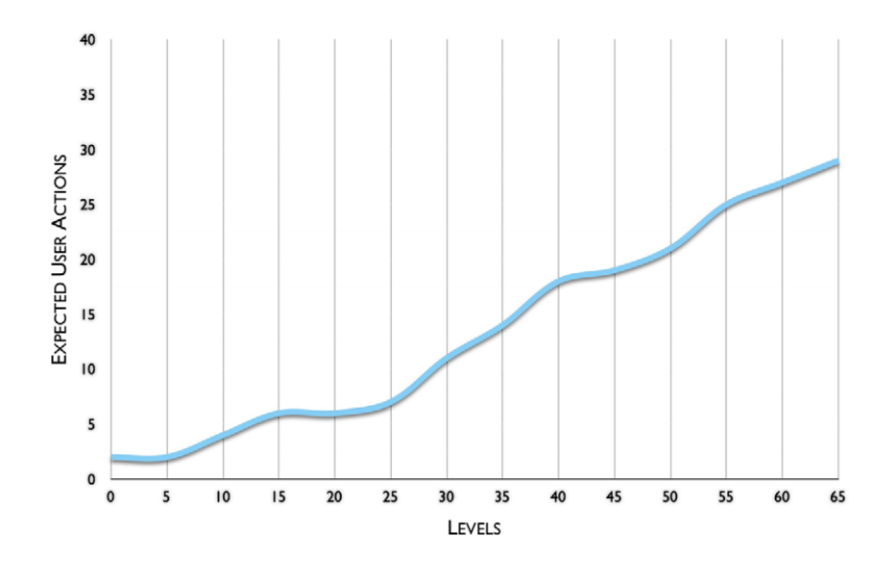
\includegraphics[scale = 0.7]{Bilder/Levels.eps}
\caption{Ansteigender Schwierigkeitsgrad bei Levels \cite{Zichermann2011}.}
\label{LevelkomplexitätBild}
\end{center}
\end{figure} 
\\
Ein gutes Level-Design kann dafür sorgen, dass der Anwender seinen Fortschritt in der Gamification-Anwendung als fesselnde Erfahrung wahrnimmt, während er Selbstbewusstsein und Erfahrung im Umgang mit der Anwendung entwickelt \cite{Zichermann2011}. Zusätzlich wird ihn durch die Levels immer ins Bewusstsein gerufen, wo seine Reise begonnen hat und sie bietet ihm auch immer einen Ausblick in die Zukunft und ein Ziel. Durch diese Rückblicke in frühere Levels wird dem Anwender die Bedeutung seines handelns bewusst, dadurch kann der Zweck der Handlung oder die Bedeutung der Tätigkeit innerhalb der gamifizierten Anwendungen für ihn steigen \cite{Zichermann2011}.
\\\\
Wichtig für das Level-Design ist es, die Levels logisch anzuordnen und sie verständlich zu machen. Eben so ist es eine gute Idee beim Design darauf zu achten, dass die Levels erweitert werden können und das sie flexibel sind. Zum Schluss ist darauf zu achten, dass die Balance der Levels stimmig ist. So gilt es die Einstiegs-Level und einsteigerfreundlich zu gestalten, während spätere Level komplex und herausfordernd sein müssen \cite{Zichermann2011}.

\subsubsection{Ranglisten}
Der Nutzen einer \textit{Rangliste} (Leaderboards) bzw. eines \textit{Highscores} ist es, eine einfache Vergleichsmöglichkeit zu schaffen. Vergleiche kann man dabei auf verschiedene Objekte beziehen wie z.B. Teams, Anwender, Länder, Gegenständen, eigene Erfolge und vieles mehr. Es überrascht nicht, dass die meisten Menschen keine Erklärungen benötigen, wenn es sich um eine Rangliste handelt. Eine geordnete Liste mit abgebildeten Punkten und nebenstehenden Namen symbolisiert uns bereits ein Ranglisten-System das keiner weiteren Erklärung bedarf (Abb.\ref{RanglistenBild}) \cite{Zichermann2011}.
\\
\begin{figure}[h!]
\begin{center}
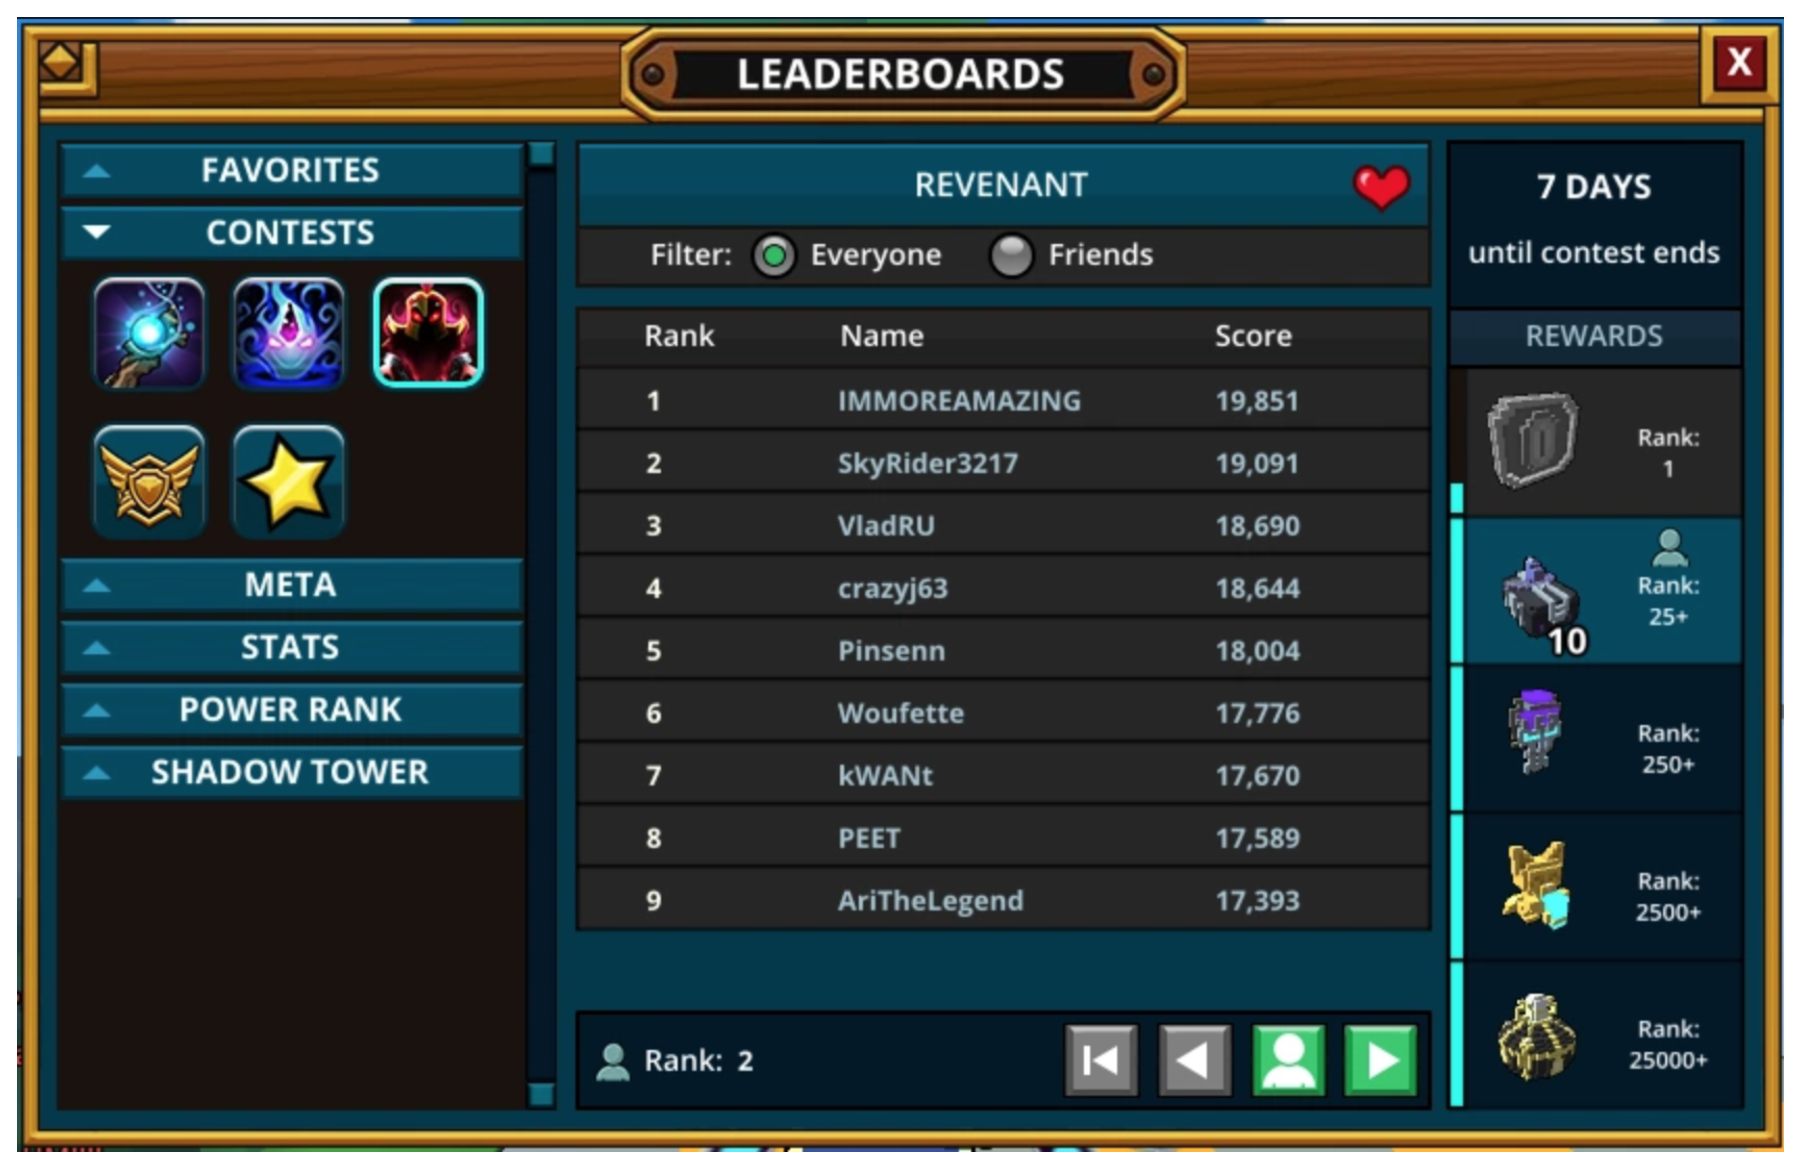
\includegraphics[scale = 0.3]{Bilder/Ranglisten.eps}
\caption{Ranglisten Besispiel entnommen aus dem Spiel \enquote{Trove} \cite{Leaderboards}.}
\label{RanglistenBild}
\end{center}
\end{figure} 
\\ 
Bei einer Rangliste handelt es sich also um eine tabellarische Auflistung von Objekten mit zugehörigem Wert, wobei die Auflistung meist absteigend sortiert ist. Als Werte eignen sich Punkte, die wir bereits am Anfang dieses Kapitels beschrieben haben. Durch die Position innerhalb der Liste wird dem Spieler oder Anwender leicht verdeutlicht, wer in der Bewertung des Systems vor ihm liegt und auch welche anderen Anwender nach ihm kommen. Durch diese verständliche Anordnung werden zwei Ziele erreicht. Zunächst werden dem Anwender eine Reihe von Zielen gegeben, in Form der anderen Anwender die über ihm stehen. Dabei ist es aber wichtig, dass die Differenz der Punkte zwischen den Anwendern nicht zu unterschiedlich ist, da diese Differenz stark abschreckend wirken kann \cite{Zichermann2011}. Als zweites Ziel kann die Erfüllung des Kompetenz Bedürfnisses erwähnt werden. Dieses wird von Anwendern befriedigt indem sie sich mit den Leuten vergleichen können die in der Rangliste schlechter abschneiden als sie selber. 
\\\\
Zichermann und Cunningham unterscheiden in ihrem Buch zwei Arten von Ranglisten, die sich aufgrund ihrer Implementierung unterscheiden. Die erste Variante ist die sogenannte \enquote{endliche Rangliste} (Finite Leaderboards)\cite{Zichermann2011}. Bei einer endlichen Rangliste sind lediglich die besten Ergebnisse aufgeführt die zusätzlich noch auf eine bestimmte Anzahl begrenzt werden. Für Anwender die sehr wettbewerbsfreudig sind kann diese limitierte Gruppe aus Elite Anwendern stark motivierend sein. Jedoch muss beim Design darauf geachtet werden, dass man einsteigerfreundlich bleibt \cite{Zichermann2011}. 
\\\\
Die zweite Variante wird als \enquote{unendliche Rangliste} (Infinite Leaderboards) bezeichnet. Diese Ranglisten enthalten den Rang aller (oder zumindest den Größtenteil von) Anwender. Bei diesen Ranglisten lohnt es sich eine Aufteilung vorzunehmen die lediglich das nähere Umfeld anzeigt. Dadurch soll der Anwender nicht durch seine Platzierung demotiviert werden \cite{Zichermann2011}. Beim Design der Rangliste ist ebenfalls auf die Erfassung der Daten zu achten. Bei den Daten die für die Berechnung des Ranges eines Anwenders verantwortlich sind kann es sich um private oder sensibele Informationen handeln die auch schwierig zu beziffern sein können \cite{Zichermann2011}. Deswegen stellt das Design einer Rangliste eine besondere Herausforderung für die Entwickler da.

\subsubsection{Abzeichen und Trophäen} 
\textit{Abzeichen} bzw. Auszeichnungen(Badges) und Trophäen sind nicht nur aus Spielen oder Gamification bekannt, sondern dienen schon seit langen für das würdigen besonderer Leistungen. Beim Militär werden Abzeichen für Leistungen wie besondere Tapferkeit vergeben und bei den Pfadfindern symbolisieren Abzeichen den Nachweis einer Fähigkeit oder Satz von Fähigkeiten. Die Abzeichen werden als Anerkennung vergeben wobei es in der Regel unwichtig ist, ob diese in der realen Welt oder im IT-Bereich vergeben werden. 
\\\\
Verwendet werden die Abzeichen bei gamifizierten Anwendungen um einen bestimmten Status zu signalisieren. Wie bei Punkten auch gelten Abzeichen als Eigentum eines Anwenders und zeichnen diesen für das ausführen einer bestimmten Tätigkeit oder das erbringen einer entsprechenden Leistung aus. Dadurch wird dem Anwender ein besonderer und spezieller \enquote{Status} zugeschrieben, den dieser Anwender erreicht hat. Damit Auszeichnungen ihre Wirkungsweise als Statussymbol entfalten können, sollte es möglich sein, die Abzeichen in einer Community zu präsentieren \cite{Zichermann2011}.    
\\\\
Neben dem symbolisieren des Status sind Abzeichen bei Menschen aber auch aus anderen Gründen so begehrt \cite{Zichermann2011}. Für viele Menschen ist das Sammeln von seltenen Objekten oder Gegenständen ein kraftvoller Antrieb. Für andere Anwender ist es ein Rausch, plötzlich und unerwartet eine Überraschung in Form eines Abzeichens durch das System zu erhalten. Daher kann es helfen, die Aufgabe bzw. das Ziel eines Abzeichens nicht unbedingt bekannt zu machen. Abzeichen können gut mit konkreten Zielen oder Leveln kombiniert werden und z.B. für das Erreichen eines bestimmten Rangs oder das Lösen einer bestimmten Aufgabe vergeben werden.
\\\\
Sind Abzeichen mit einer schweren Herausforderung verbunden, kann man diese auch als Trophäen realisieren. Durch Trophäen können einem Anwender Triumph und Sieg vermittelt werden. Da Trophäen einen höheren subjektiven Stellenwert haben als Abzeichen, symbolisieren diese auch den Stolz des ausgezeichneten Anwenders. Zu vergleichen sind Trophäen mit Sportpokalen oder Jagdtrophäen \cite{Zichermann2011}.   
\\
\begin{figure}[h!]
\begin{center}
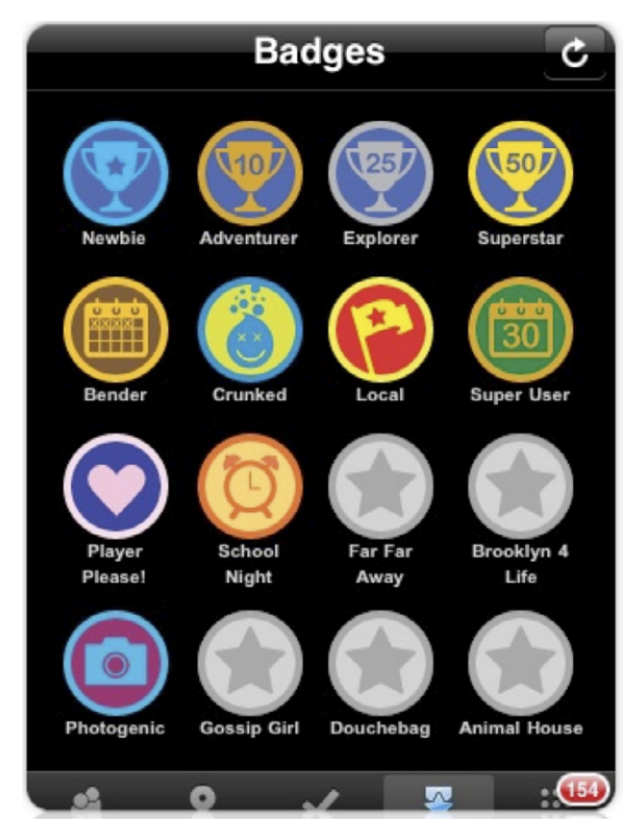
\includegraphics[scale = 0.45]{Bilder/Abzeichen.eps}
\caption{Abzeichen aus der bekannten Gamification-Anwendung \enquote{Fourscare} \cite{Zichermann2011}.}
\label{RanglistenBild}
\end{center}
\end{figure} 
\subsection{Zusammenfassung}
In diesem Kapitel haben wir uns mit den Grundlagen der Gamification auseinander gesetzt. Gamification wird wie wir bereits erwähnt haben genutzt um Anwendungen, Prozesse oder Systeme umzugestalten und sie durch den Einsatz von Spielelementen so zu gestalten, dass sie für den Anwender motivierender wirken. Dabei darf eine Gamification-Anwendung aber nicht als ein Spiel (Game) betrachtet werden. Durch die Unterschiede wie z.B. die Zweckmäßigkeit der Gamification-Anwendung oder das Fehlen von Gameplay ist zu erkennen, dass die Gamification anders einzuordnen ist als ein Spiel. Jedoch sind die Übergänge zwischen Games und Gamification fließend weshalb es möglich ist, die verschiedenen Prinzipien und Verfahren die aus der Spieleentwicklung bekannt sind auch für die Gamification einzusetzen.
\\\\
Die verschiedenen Verfahren die aus der Spieleentwicklung für die Gamification eingesetzt werden können wurden in diesem Kapitel durch die Game-Design Elemente zusammengefasst. Diese Elemente unterstützen nicht nur die Entwickler bei der Entwicklung und der Konzeptionierung einer gamifizierten Anwendung, sondern wirken sich auch direkt auf den Anwender aus. Die Game-Design Elemente teilen sich in die fünf Ebenen: \textit{Interface-Elemente}, \textit{Game-Mechaniken}, \textit{Game-Design Grundsätze}, \textit{Game-Design Modelle} und \textit{Game-Design Methoden} auf. Durch die Einstufung der Game-Design Elemente in fünf abstrakte Ebenen lassen sich die Abhängigkeiten der Elemente deutlich darstellen. So hängt die erste Abstraktionsebene, die Interface-Elemente stark von der zweiten Ebene der Game-Mechaniken ab.
\\\\
Als zentrales Element des Game-Design wurden die Game-Design Grundsätze ermittelt. Diese Grundsätze beschreiben wie die intrinsische Motivation bei Spielen oder gamifizierten Anwendung zustande kommt. Die intrinsische Motivation wird durch  die Befriedigung der Grundbedürfnisse: \textit{Kompetenz}, \textit{Autonomie}, \textit{Eingebundenheit} und \textit{Zweck} erreicht. Diese Bedürfnisse müssen indirekt über den Einsatz von Game-Mechaniken und Interface-Elemente angesprochen werden. Desto besser die gamifizierte Anwendung diese Bedürfnisse befriedigt, desto motivierender wirkt die Anwendung. Beim Design einer gamifizierten Anwendung ist es also wichtig, diese Bedürfnisse in den Vordergrund zu stellen und die Game-Mechaniken und Interface-Elemente nach diesen menschlichen Bedürfnissen auszurichten.
\\\\  
Durch die Game-Design Modelle werden die Entwickler bei der Konzeption einer gamifizierten Anwendung unterstützt. So bringt das MDA-Modell z.B. die Ansichten von Entwickler und Anwender zusammen und unterteilt die Anwendung in drei Komponenten: \textit{Mechanik}, \textit{Dynamik} und \textit{Ästhetik}. Durch diese Einteilung können Abhängigkeiten der Komponenten untereinander leichter identifiziert und entwickelt werden. Ein weiteres Modell das in dieser Arbeit aufgeführt wurde ist das Modell der Skill Atoms. Bei diesem Modell können einzelne Herausforderungen, Spieleraktionen und Feedback-Mechanismen gestaltet und getestet werden. Das Letzte Modell das wir in dieser Arbeit besprochen haben war das CEGE-Modell (Core Elements of the Gaming Experience). Dieses Modell teilt die unterschiedlichen Aspekte eines Spieles auf, wie \textit{Umgebung}, \textit{Gameplay}, \textit{Eigentum} und \textit{Kontrolle} (um nur ein paar zu nennen). Dadurch kann der Entwickler prüfen, ob Aspekte während des Design-Prozesses übersehen oder vernachlässigt wurden um diese zu verbessern. Durch diese Modelle können Gamification-Anwendungen effizienter und risikofreier entwickelt werden.    
\\\\
Die Game-Design Methode sorgt für das Aufbrechen des Game-Designs und teilt diesen Prozess in sinnvolle Schritte ein. Durch die passende Methode im Game-Design können sich Entwickler schrittweise an die Planung und Konzeption der sogenannten \textit{Player Experience} machen und sich auf die Ziele der Anwender fokussieren. Für diese Arbeit hat man sich dazu entschieden die sogenannte \textit{Player-Centric Design} Methode zu betrachten. Die Anwender werden beim Player-Centirc Design in den Vordergrund gestellt und es wird ermittelt, wie die Ziele des Anwenders aussehen und wie diese mit den Geschäftszielen der Anwendung verbunden werden kann.    
\\\\
Zum Schluss wurden in diesem Kapitel die Game-Mechaniken und Interface-Elemente beschrieben und deren Funktionsweise aufgeführt. Bei den Game-Mechaniken handelt es sich wie wir festgestellt haben um regelbasierte System, die es einem Anwender erlauben, die Eigenschaften der gamifizierten Anwendung durch Feedback-Mechanismen zu erforschen und zu erlernen. Für diese Arbeit haben wir uns auf die zwölf Game-Mechaniken von Zichermann und Cunningham \cite{Zichermann2011} konzentriert, da diese sich besonders gut für Gamification eignen und sie einen guten Überblick verschaffen. Durch diese Auflistung an verschiedenen Mechaniken können für unser Konzept, dass im nächsten Kapitel folgt, die passenden Möglichkeiten herausgearbeitet werden. Die Interface-Elemente die bei Gamification verwendet werden, können allgemein in die vier Kategorien eingeteilt werden: \textit{Punkte}, \textit{Ranglisten}, \textit{Abzeichen} und \textit{Level}. Diese Game-Charaktere werden dem Anwender zuerst bewusst und müssen dementsprechend entworfen werden. Diese Interface-Elemente sollen dem Anwender über seinen Fortschritt informieren und ihn auf einer emotionalen Ebene ansprechen. Die Interface-Elemente sollen aber nicht als Belohnung gesehen werden. Das Feedback an den Anwender über seine Leistung und sein Optimierungspotential stehen bei den Interface-Elementen im Vordergrund. 
\newpage
\section{Konzeption}
\label{Konzeption}
Im Kapitel \ref{Zusammenfassung des Knowledge Managements} wurde die Anforderungsliste für den Gamification Teil aufgestellt. Die Anforderungen waren, \textit{Motivation durch Belohnungen erhöhen}, \textit{Fähigkeiten des WE-Prozesses verbessern} und \textit{Auslöser finden und entwickeln}. Diese Anforderungen sollen nun bei der Konzeption einer gamifizierten Confluence Anwendung zur Hilfe genommen werden. Hierfür wird die Anforderung \textit{Motivation durch Belohnungen erhöhen} jedoch in \textit{Motivation durch Feedback erhöhen} umgewandelt, da Belohnungen zur Hemmung der Kreativität führen und extrinsische statt intrinsische Motivation gefördert wird, wie wir in Kapitel \ref{Punkte und Belohnungen} ermittelt haben. 
\\\\
Zusätzlich zu den Anforderungen wurde in Kapitel \ref{Zeitersparnis} erwähnt, dass es sich bei Wissensbasen um Möglichkeiten handelt, Zeitersparnisse zu generieren. Diese Erkenntnis zählt zu den größten Vorteilen des Knowledge Managements und muss dem Anwender daher besser vermittelt werden. Aus diesem Grund soll die Anforderungsliste um die Anforderung, \textit{Zeitersparniss soll besser vermittelt werden} erweitert werden. Diese neue Anforderung ist deswegen so relevant, da sie eine wichtige Quelle für die intrinsische Motivation darstellt.
\\\\
In diesem Kapitel soll nun das Konzept aus den Anforderungen und Erkenntnisse der vorangegangenen Kapiteln erstellt werden. Dieses Konzept wird die entsprechenden Gamification Elemente enthalten, die im weiteren Verlauf dieser Arbeit für die Umsetzung der Modifikationen in der Confluence Wiki verwendet werden. Dafür werden die Anforderungen mit den bisherigen behandelten Gamification Mechaniken und den Interface-Elementen abgeglichen. Daraus lässt sich dann bestimmen, welche Elemente sich für die Erweiterung der Confluence Wiki eignen. Bei der Entwicklung des Konzepts ist darauf zu achten, dass auf die Ursachen des derzeitigen Anwenderverhaltens eingegangen wird. Das derzeitige Anwenderverhalten lässt sich kurz zusammenfassen als, \textit{Anwender erfassen zu wenig Informationen in der Confluence Wiki}. Mit diesem Konzept sollte es nach Abschluss dieser Entwicklungsphase möglich sein, die Frage zu beantworten: \textit{Wie kann Gamification genutzt werden um das Eintragen von Informationen in die Wiki zur Gewohnheit des Anwenders zu machen} ?

\subsection{Erforschen der Player Goals und Geschäftsziele}
Durch die Design-Methode des Player-Centirc Designs, die wir in Kapitel \ref{Player-Centric Methode} beschrieben haben wissen wir, dass die Anwender beim Entwurf einer gamifizierten Lösung im Mittelpunkt stehen. Somit ist es also erforderlich, sich mit dem Anwender und seinen Zielen auseinander zu setzen. Der Anwender wird in der  Konzeptionsphase als Player bezeichnet. Es müssen jetzt also die Ziele des Players (Player Goals) ermittelt werden. 
\\\\
Neben den Zielen der Anwender ist es ebenfalls erforderlich, die Geschäftsziele (Business Objectives) für die Modifikationen an der Confluence Wiki zu definieren. Dies ist ein besonders wichtiger Punkt, da Gamification ein neuer Trend ist, dem sich viele Firmen zu nutzen machen wollen. Dabei werden häufig die Geschäftsziele außer Acht gelassen was dazu führt, dass diese Gamification-Projekte dann scheitern \cite{gamificationDefinition}. Hierfür reicht es aber nicht, die Geschäftsziele grob zu definieren wie \textit{mehr Customer Traffic auf der gamifizierten Website}. Die Geschäftsziele müssen als Metriken oder Kennzahlen erfasst werden und dies so spezifisch wie möglich \cite{gamificationDefinition}. Die Metriken und Kennzahlen für die Geschäftsziele werden ebenfalls in diesem Kapitel festgelegt.
\subsubsection{Bestimmen der Zielgruppe}
\label{Zielgruppe}
Zunächst muss die Zielgruppe bestimmt werden die als Player für die gamifizierte Confluence Wiki infrage kommt. Bei Gamification unterscheidet man in der Regel zwischen drei verschiedenen Zielgruppen. Die Zielgruppen teilen sich dabei in \textit{Kunden}, \textit{Mitarbeiter} und \textit{Communities} auf \cite{gamificationDefinition}. In unserem Fall sind die \textit{Mitarbeiter} die Player unserer gamifizierten Confluence Wiki. Über die Player sind jetzt auch weitere Informationen bekannt. So liegt das Alter der Player zwischen 25 und 55 Jahren wobei ca. 50 \% der Mitarbeiter um die 30 Jahre alt ist. Von den Playern sind ca. 80 \% männlich und sie sind entweder als Consultant oder Senior Consultant angestellt. Die Zielgruppe für die gamifizierte Confluence Anwendung sind also die Consultants. 
\\\\
Aus den vorliegenden Informationen können bereits wertvolle Hinweise für das Konzept gewonnen werden. Circa 50 \% der Mitarbeiter sind um die 30 Jahre alt und sind somit zu einer großen Wahrscheinlichkeit auch mit Videospielen aufgewachsen. Dadurch kann man vermuten, dass dieser Teil der Player besonders positiv auf die Spielmechaniken reagieren wird \cite{Persona2018}. Ein weiteres markantes Merkmal ist der große Anteil an männlichen Mitarbeitern. Männer sind in der Regel eher Wettkampf orientiert während Frauen mehr auf soziale Mechaniken ansprechen \cite{Persona2018}. Also kann man bei einer Anwendung, die hauptsächlich von Männern genutzt wird, erfolge erzielen, in dem man Wettkampf-Bedingungen schafft. Da wir nun die Zielgruppe ermittelt haben, wird der WE-Prozess nochmal unter Berücksichtigung der Zielgruppe analysiert. 
\\\\
Der Wissenserfassungsprozess kann in vier kleinere Handlungen des Players aufgeteilt werden. Diese wären \textit{schreiben}, \textit{lesen}, \textit{suchen} und \textit{kommentieren}. Diese Handlungen stellen die Interaktion des Players mit der Confluence Wiki dar und werden nun genutzt, um die Player Goals zu bestimmen. Zusätzlich werden Statistiken über die Interaktionen der letzten Monate geführt um Kennzahlen für die Bestimmung der Geschäftsziele zu erhalten. Es kann also ermittelt werden, wie viele Anwender zu einem bestimmten Zeitpunkt Informationen in die Confluence Wiki \textit{geschrieben} haben oder wie viele Einträge bereits \textit{gelesen} bzw. aufgerufen wurden. Die Kennzahlen anhand derer die Geschäftsziele ausgelegt werden, werden in Kapitel \ref{Geschäftsziele} beschrieben.

\subsubsection{Erstellung und Analyse des Fragebogens}
Um ein besseres Verständnis für die Ziele und Bedürfnisse der Player zu bekommen, wurde eine Firmeninterne Umfrage durchgeführt. Die Umfrage bezog sich auf die Interaktionen der Player mit der Confluence Wiki, also auf die Aktionen \textit{schreiben}, \textit{lesen}, \textit{suchen} und \textit{kommentieren}. Die Fragen wurden absichtlich kurz gehalten, um Mitarbeiter zu motivieren, sich an der Umfrage zu beteiligen. Die Umfrage besteht aus drei Fragen die für alle vier Aktionen (schreiben, lesen, suchen, kommentieren) gestellt wurden, was zu insgesamt zwölf Fragen führt.
\begin{description}
   \item[Die Fragen lauten:]~\par
   \begin{enumerate}
      \item Was gefällt euch, wenn ihr in Confluence einen Eintrag schreibt?
      \item Was gefällt euch \textbf{NICHT}, wenn ihr in Confluence einen Eintrag schreibt?
      \item Wie könnte man eurer Meinung nach das Schreiben verbessern?
      
      \item Was gefällt euch, wenn ihr in Confluence einen Eintrag liest?
      \item Was gefällt euch \textbf{NICHT}, wenn ihr in Confluence einen Eintrag liest?
      \item Wie könnte man eurer Meinung nach das Lesen verbessern?
      
      \item Was gefällt euch, wenn ihr in Confluence einen Eintrag sucht?
      \item Was gefällt euch \textbf{NICHT}, wenn ihr in Confluence einen Eintrag sucht?
      \item Wie könnte man eurer Meinung nach das Suchen verbessern?
      
      \item Was gefällt euch, wenn ihr in Confluence einen Eintrag kommentiert?
      \item Was gefällt euch \textbf{NICHT}, wenn ihr in Confluence einen Eintrag kommentiert?
      \item Wie könnte man eurer Meinung nach das Kommentieren verbessern?
   \end{enumerate}
\end{description}
Die Fragen sollen Aufschluss darüber geben, über welche positiven und negativen Eigenschaften die Confluence Wiki zum momentanen Zeitpunkt verfügt. Außerdem soll ermittelt werden, welche Verbesserungen sich die Player wünschen. Man könnte argumentieren, dass die Frage nach positiven Eigenschaften in der Confluence Wiki nicht Teil dieser Arbeit sein sollte. Da das Ziel dieser Arbeit darin besteht, die negativen Aspekte der Confluence Wiki mit Gamification zu optimieren. Aber gerade deswegen sind Fragen nach positiven Eindrücken wichtig. Die positiven Aspekte der Confluence Wiki sollen bei der Gamification Umsetzung von Confluence wenn möglich nicht verändert werden, sie ermöglichen aber zusätzliche Einblicke in die Verhaltensweise des Players, da mit den Fragen zu den positiven Aspekten eine Übersicht entsteht, was dem Player innerhalb des Prozesses wichtig ist.
\\\\
\textbf{Umfrage Evaluierung des Schreib-Prozesses}\\
Aus der Umfrage ergaben sich folgende Ergebnisse für den Schreib-Prozess in Confluence. Es wurde von den Player als positiv gewertet, dass das Erstellen eines neuen Eintrages in die Confluence Wiki einfach und schnell funktioniert. Man kann immer über einen einzigen Klick an Ort und Stelle einen neuen Eintrag generieren, wie in Abbildung \ref{ConfluenceEintragErstellen} zu sehen ist. Eine weitere positive Eigenschaft von Confluence ist es, dass die Einträge sichtbar für alle Mitarbeiter sind und es den Playern ermöglicht wird sofort nach der Erstellung des Eintrages darauf zuzugreifen. Außerdem wurden die verschiedenen Struktur Möglichkeiten in Form von Tabellen oder Inhaltsverzeichnisse ebenfalls als positiv gewertet. Dadurch lassen sich Einträge in der Anwendung unterschiedlich anordnen und man kann ihnen Sonderfunktionen zuweisen wie z.B. das Bestätigen einer Checkliste die als eine einfache Tabelle umgesetzt wird.
\begin{figure}[h!]
\begin{center}
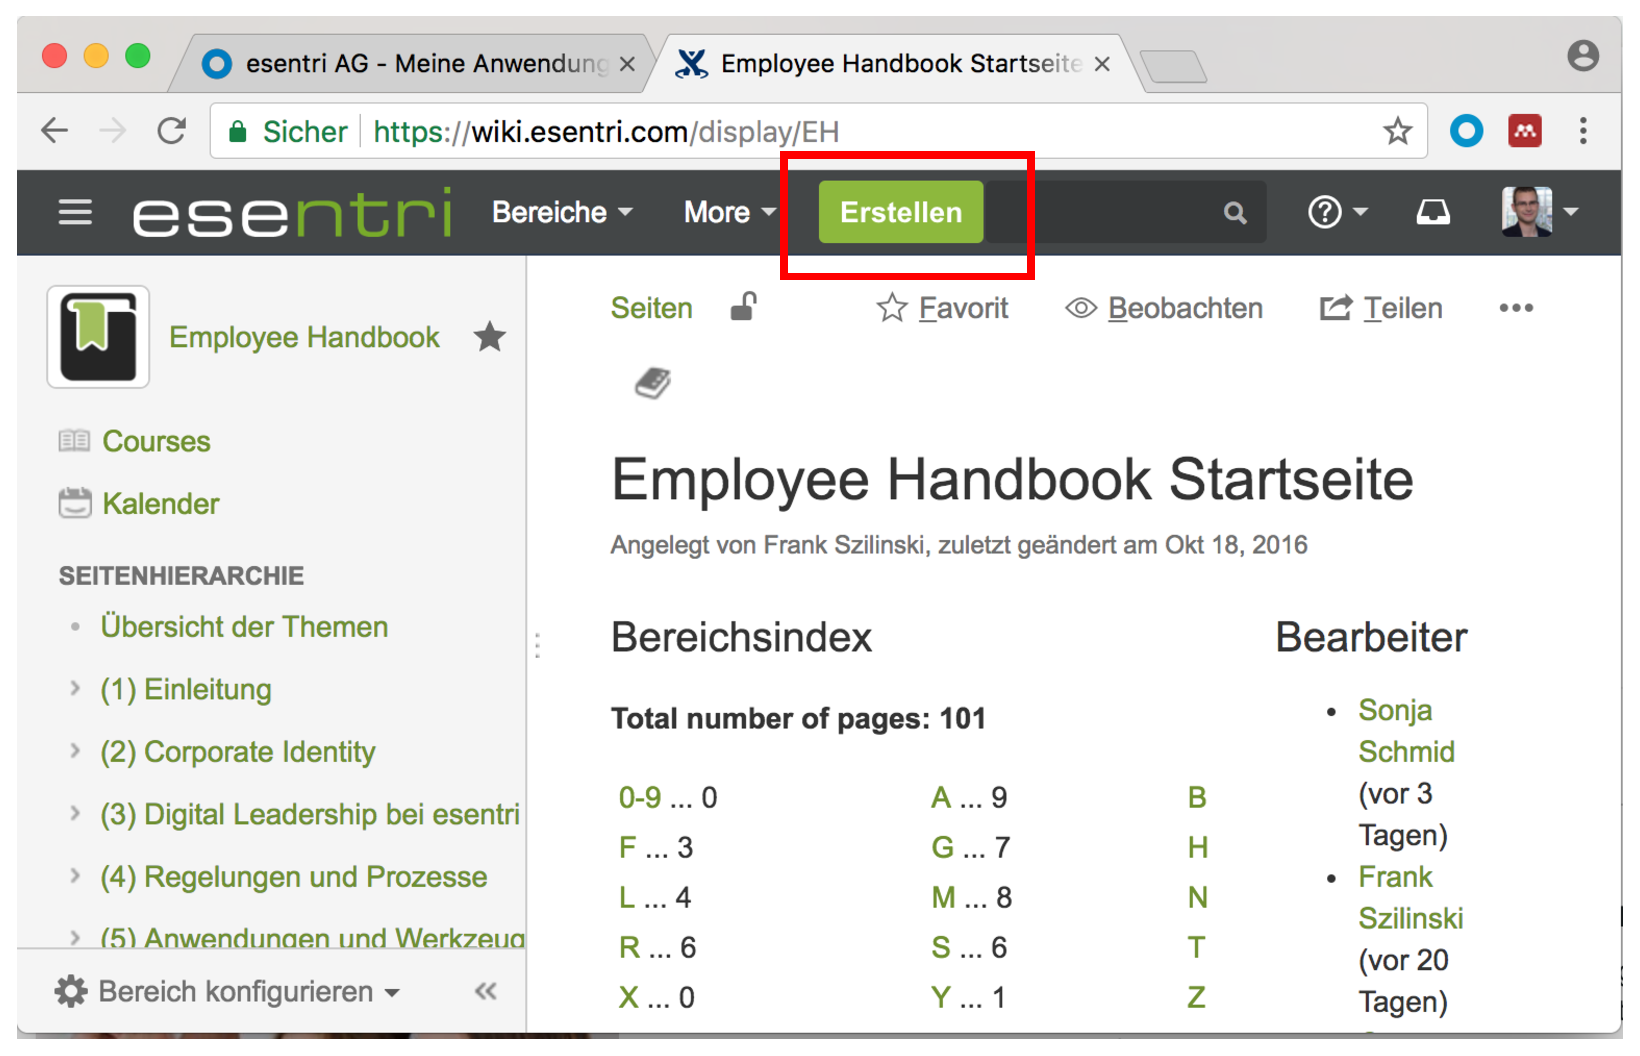
\includegraphics[scale = 0.4]{Bilder/ConfluenceStart.eps}
\caption{Sichtweise der Player auf die Confluence Startseite.}
\label{ConfluenceEintragErstellen}
\end{center}
\end{figure} 
\\\\
Beschwert haben sich die Player über einen eingeschränkten Editor und über die Anordnung der Editor-Funktionen. Des weiteren gaben die Player im Fragebogen an, dass die Confluence Wiki unübersichtlich sei und die Features nicht richtig genutzt werden. Die Optik und das Layout der Seite wurden ebenfalls als negative Eigenschaften gewertet. Worüber sich die Player weiterhin beschwert haben war, dass die Zuordnung von neu erstellten Einträgen schwierig ist. Weiß ein Player nicht genau, wo der Eintrag beim erstellen eingeordnet werden soll, so kann das Verschieben dieses Eintrags später für Problem sorgen.
\\\\
Die Verbesserungen die von den Playern vorgeschlagen wurden beinhalten unter anderem, dass der Editor um weitere Features erweitert wird und das diese auch sinnvoll gruppiert werden. Hinzukommen sollen außerdem noch mehr Freiheiten für die Gestaltung und Strukturierung des Eintrages. Es wird gewünscht das Layout zu verbessern und das beim Schreiben intelligente Vorschläge gemacht werden, wo der Eintrag einzuordnen ist.
\\\\
\textbf{Umfrage Evaluierung des Lese-Prozesses}\\
Die Antworten auf die Fragen zum Lese-Prozess ergaben, dass die Player zwischen den Aktivitäten des Lesens von Einträgen und Suchen von Einträgen keine Unterscheidung treffen. So hat die Frage \enquote{\textit{Was gefällt euch, wenn ihr in Confluence einen Eintrag liest?}} gezeigt, dass der Lese-Prozess nur dann als positiv empfunden wird, wenn die Einträge die bei der Suche zurückgeliefert werden auch die Antworten auf spezifische Problemstellungen des Players enthält. Hierfür ist ein strukturierter Überblick hilfreich und kurzgehaltene gut strukturierte Inhalte. Dadurch kann der Player effektiv bestimmen, ob der Eintrag für ihn relevant ist. 
\\\\
Bei der Umfrage gaben die Player auf die Frage \enquote{\textit{Was gefällt euch \textbf{NICHT}, wenn ihr in Confluence einen Eintrag liest?}} folgende Antworten. Die Player führten als negativen Aspekt auf, dass es erforderlich ist den Autor bei unverständlichen Einträgen direkt anzusprechen. Diese Tatsache ist besonders frustrierend, da Confluence über eine Kommentier-Funktion verfügt die gerade für Rückfragen gedacht ist. Diese wird von den Playern jedoch nicht richtig verwendet. Die Volltextsuche von Confluence wurde ebenfalls bemängelt. Die Volltextsuche liefert dem Player als Ergebnis auf seine Anfrage zu viele Einträge, die alle nach dem passenden Inhalt durchsucht werden müssen, was den Playern verärgert. Der letzte Kritikpunkt, der von den Playern aufgeführt wurde, betrifft die Aktualität einiger Einträge. Wie wir bereits in Kapitel \ref{Zeitersparnis} ermittelt haben, ist Aktualität ein wichtiges Kriterium des Knowledge Managements. Als solches ist es verständlich, wenn Player durch veraltete Einträge verwirrt werden, da Player nicht unterscheiden können, ob die Inhalte noch relevant sind oder nicht. 
\\\\
Als Verbesserungsvorschläge für den Lese-Prozess schlagen die Player ein Feature vor, dass ihnen dabei hilft Informationen schneller zu finden. Dieses Feature sollte in der Lage sein, dem Player weitere intelligente Vorschläge zu machen, wo sich die angefragten Informationen eventuell ebenfalls befinden könnten. Dieser Vorschlag verdeutlicht wie eng der Lese- und Such-Prozess in den Augen der Player zusammenhängt. Eine weitere Idee war es die Anzahl von Bildern bzw. Videos innerhalb von Einträgen zu erhöhen. Zwar ist es in der Confluence Wiki möglich Bilder hochzuladen, wie die Umfrage aber zeigt, wird dieses Feature zu selten genutzt. Ein möglicher Ansatz wäre eine Schnappschuss-Funktion die das Bild direkt aus dem Display des Players hochlädt.
\\\\
\textbf{Umfrage Evaluierung der Such-Funktion}\\
Obwohl der Such-Prozess bereits im vorherigen Abschnitt erwähnt und zum Teil auch analysiert wurde, werden die positiven Eigenschaften der Suche hier nochmal genauer analysiert. Die Suche in der Confluence Anwendung bietet beim Eingeben der Anfrage bereits Stichworte (Abb.\ref{Sucheingabe}). Dieses Feature ist zwar nützlich, funktioniert nach Angaben der Player aber nur, wenn man weiß wonach man sucht. Dies liegt oft auch daran, dass die Einträge falsch oder mehrfach benannt sind. Wenn die gewöhnliche Such-Funktion von Confluence nicht ausreicht, verwenden die Player die Volltextsuch-Funktion. Diese liefert zwar zu viele Beiträge, ist aber leicht zu bedienen und verständlich.
\\
\begin{figure}[h!]
\begin{center}
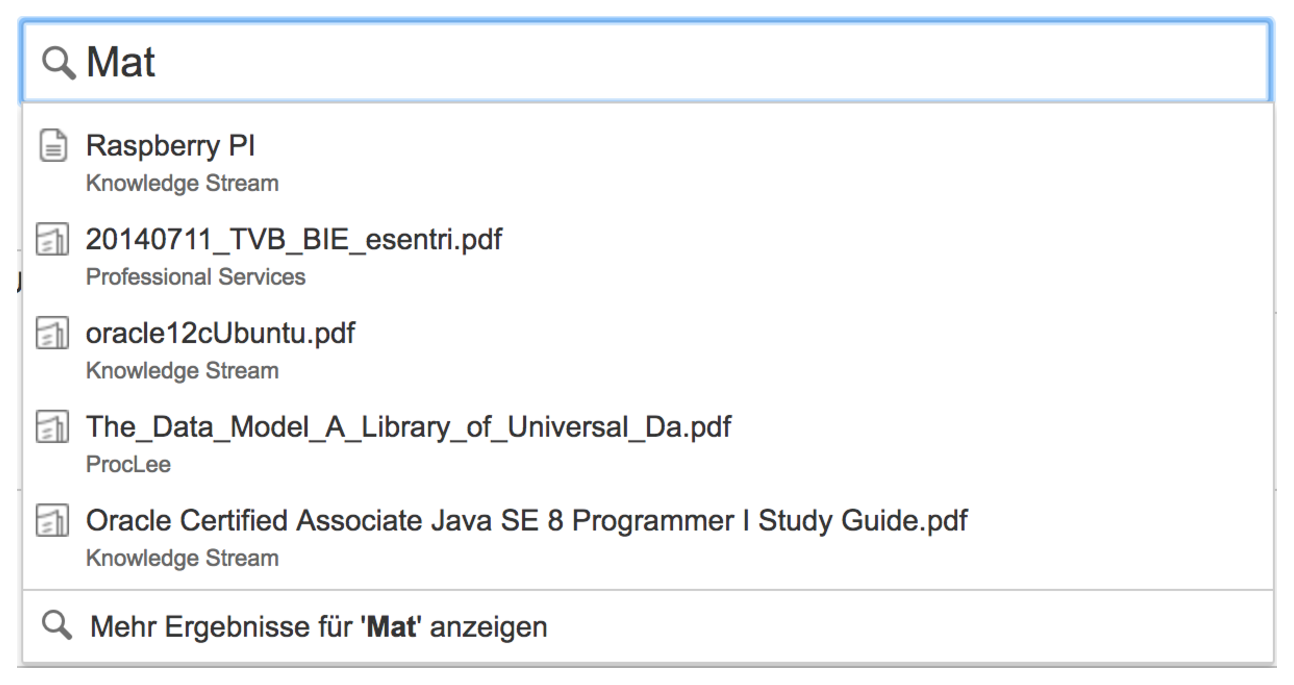
\includegraphics[scale = 0.4]{Bilder/Sucheingabe.eps}
\caption{Der Player wird bei der Suche über Stichwörter unterstützt.}
\label{Sucheingabe}
\end{center}
\end{figure}
\\
Als negativ wurde von den Player bei der Such-Funktion bewertet, dass die Funktion wie gesagt zu viele Ergebnisse liefert und man bereits vor der Suche eigentlich wissen muss, wie die Inhalte benannt wurden. Als eine weitere negative Eigenschaft der Suche wurde von den Playern vermerkt, dass Inhalte zu Themen nicht gefunden werden, weil die entsprechenden Suchbegriffe nicht in die Anfrage mit aufgenommen wurden. Diese Synonyme stellen für die Player immer wieder ein Problem dar, da Player nie genau wissen können, welche Suchbegriffe ihnen die besten Ergebnisse liefern. 
\\\\
Die Such-Funktion, die bei Confluence zum Einsatz kommt verfügt nach Ansicht der Player über klare Mängel. Als solches wünschen die Player sich eine Verbesserung dieser Funktion. Dabei wäre es für die Player schon ausreichend, wenn die Such-Funktion auf Suchbegriffe toleranter reagieren würde. Dadurch könnten Einträge besser gefunden werden. Player haben auch vorgeschlagen, den Suchalgorithmus zu verbessern und die semantischen Beziehungen der Suchbegriffe zwischen einander herzustellen. So könnten inhaltliche Bezüge bei Suchergebnissen dargestellt werden.
\\\\
\textbf{Umfrage Evaluierung der Kommentier-Funktion}\\
Die Kommentier-Funktion von Confluence erlaubt es, für jeden Eintrag ein Kommentar abzusetzen. Durch diese Funktion können z.B. Rückfragen des Lesers an den Autor des Eintrages übermittelt werden oder es können Verbesserungsvorschläge gemacht werden. Die Kommentier-Funktion ist zwar praktisch und unterstützt die Player vor allem beim verteilten Arbeiten, dennoch wird diese Funktion kaum von den Playern verwendet. Wieso diese Funktion von den Playern nicht häufiger genutzt wird, konnte mit dem Fragebogen nicht geklärt werden. Es liegt allerdings die Vermutung nah, dass es für die Player auch bei dieser Eigenschaft von Confluence keinen Anreiz gibt, sie zu verwenden. Für diese Arbeit soll die Kommentier-Funktion aber vernachlässigt werden, da sie für den eigentlichen Wissenserfassungsprozess keine Rolle spielt.

\subsubsection{Ermitteln der Player Goals}
Aus der Umfrage-Evaluierung können nun die Player Goals genauer bestimmt werden. Aus den Antworten der internen Umfrage soll nun auf die Absichten des Players bzw. auf die Player Goals, geschlossen werden. Diese Überleitung,
von Antworten auf Player Goals mag zunächst ungenau und willkürlich erscheinen. Doch die Player Goals dienen dazu, eine spezifische Richtung für die Konzeption festzulegen und müssen deswegen auch nicht zu hundert Prozent zutreffen. Für diese Arbeit und für die Gamifizierung der Confluence Wiki reichen unsere Annahmen und Vermutung im ersten Ansatz der Konzeptionsphase aus. Außerdem werden die Player Goals indirekt über die Umsetzung der von den Playern gewünschten Verbesserungen adressiert. Aus diesen Gründen ist es irrelevant, dass die Player Goals aus Annahmen geformt werden.
\\\\
\textbf{Player Goal: Player wollen Inhalte schnell eintragen}\\
Die Antworten aus der Umfrage haben verdeutlicht, dass es den Playern wichtig ist, ihre Informationen so schnell wie möglich in die Wiki einzutragen. Diese Erkenntnis wurde aus den positiven Schreib-Eigenschaften entnommen. Aus diesem Grund ist es für eine erfolgreiche Gamifizierung nötig, die Editor Funktionen so auszulegen, dass die Player schnell und routiniert ihre Einträge erstellen und bearbeiten können. Hierfür müssen die Funktionen des Editors bewertet werden. Die Funktionen, die von den Playern häufiger verwendet werden, müssen leicht zu erreichen und schnell zu finden sein.
\\\\
\textbf{Player Goal: Player wollen schnell entscheiden, ob Inhalte vorhanden sind, die sie suchen}\\
Eine der wichtigsten Erkenntnisse, die durch die Umfrage gewonnen wurde ist die Tatsache, dass für die Player, das Suchen und Finden von Beiträgen gleichzusetzen ist mit dem Lesen dieser Beiträge. Findet ein Player durch die Suche also die Beiträge die seine Fragen beantworten, wird dieser Beitrag auch gelesen. Wird also die Treffsicherheit der Suchfunktion verbessert, werden automatisch mehr Beiträge von den Playern konsumiert. Neben der Optimierung der Suchfunktion wäre es auch weiter denkbar, eine Funktion zu implementieren die dem Player alternative Vorschläge zu den gesuchten Inhalten gibt. Bei der Suche will der Player mit so wenigen Klicks wie möglich an sein Ziel kommen. Wird einmal die Suchanfrage gestartet so erwartet der Player ein entsprechendes Ergebnis, welches ihm präsentiert wird. Jegliches durchsuchen der Suchergebnisse wird vom Player daher verständlicherweise als Hindernis wahrgenommen.
\\\\
\textbf{Player Goal: Player haben das Ziel, dass ihre Einträge gelesen werden sollen}\\
Wie die Umfrage gezeigt hat, ist die richtige Einordnung von Einträgen bzw. Artikeln ein weiterer wichtiger Punkt für den Player. So kann also behauptet werden, dass die Player über ein inhärentes Interesse verfügen, ihre Einträge auffindbar zu machen, so das ihre Inhalte und Informationen von anderen Playern ebenfalls wahrgenommen werden. Dieses Ziel der Player, ihr wissen mit anderen zu teilen, ist letzten Endes auch ausschlaggebend für ein erfolgreiches Knowledge Management. Durch die Confluence Wiki muss dem Player nun spürbar vermittelt werden, dass er bei dem Erreichen seines Ziels von der Wiki unterstützt wird. Durch eine bessere Zuordnung wird nicht nur auf die Ziele und wünsche des Players eingegangen. Nebenbei werden auch die Ergebnisse der Suchfunktion verbessert. Dadurch wird das Erlebnis der Suche in Confluence optimiert.
\\\\
Mit diesen drei Zielen der Player haben wir nun eine Grundlage für unser Konzept. Dabei gibt es noch weitere Player Goals die hier aber nicht weiter aufgeführt werden sollen, da man sich darauf geeinigt hat, sich auf diese drei Player Goals zu konzentrieren. Diese Entscheidung wurde beschlossen, um den Rahmen dieser Arbeit nicht noch weiter auszudehnen. Außerdem sind die hier aufgeführten Player Goals diejenigen, die wohl den größten Einfluss auf die Player ausüben, da sie starke Überschneidungen mit den Aktivitäten des \textit{Schreibens}, \textit{Lesens} und \textit{Suchen} aufweisen. Und diese wiederum sind die wichtigsten Bestandteile des Wissenserfassungsprozesses.
\\\\
Als Nächstes müssen nun die Geschäftsziele ermittelt werden. Aus der Kombination von Geschäftszielen und Player Goals sollen im Anschluss die \textit{Gamification-Ziele} bestimmt werden. Diese wiederum ergeben sich aus der Schnittmenge von Player Goals und Geschäftszielen.  
 
\subsubsection{Geschäftsziele erläutern und bestimmen}
\label{Geschäftsziele}
In diesem Abschnitt sollen nun die Geschäftsziele (Business Objectives) für diese Arbeit erläutert und bestimmt werden. Die Geschäftsziele sind die Schlüsselzahlen und Ergebnisse, die das Unternehmen mit Hilfe von Gamification verbessern will. Grob kann das Ziel dieser Arbeit formuliert werden als:
\\\\
\textit{Mitarbeiter sollen mehr Beiträge in die Confluence Wiki eintragen und lesen.}
\\\\
Da diese Formulierung aber zu vage ist, um aus ihr bestimmen zu können, wie dieses Geschäftsziel erreicht werden kann, muss dieses Ziel zunächst quantifiziert werden. Im ersten Schritt müssen nun die entsprechenden Kennzahlen und Geschäftsmetriken, mit denen sich dieses Ziel messen lässt, ermittelt werden. Über diese Metriken kann im Anschluss an das Gamifiaction-Projekt ermittelt werden, ob die Umsetzung des Projektes erfolgreich war oder nicht. Als Geschäftsmetriken können verschiedene Kennzahlen genutzt werden. Einige Metriken enthalten den \textit{Umsatz}, \textit{tägliche aktive Besucher} oder \textit{Registrierungen} um hier ein paar Beispiele zu nennen \cite{Dashboard}. Die Kennzahlen die für die Geschäftsmetriken gewählt werden, müssen Aussagen über den Erfolg des Prozesses, für den sie gewählt wurden, ermöglichen. Wachsende Kennzahlen bedeuten eine Verbesserung des Prozessablaufs und stellen somit auch eine Verbesserung der Produktivität der Firma dar. Beim Auswählen der Geschäftsmetriken ist darauf zu achten, dass sie quantifizierbar und nach ihrer Wichtigkeit geordnet sind \cite{Dashboard}.
\\\\
Wie wir bereits in Kapitel \ref{Zielgruppe} festgelegt haben, orientieren sich die Geschäftsmetriken an den verschiedenen Handlungen des Players wie \textit{Schreiben}, \textit{Lesen} und \textit{Suchen}. Zum Erstellen der Geschäftsmetriken muss nun also erforscht werden, wie viele Einträge in die Confluence Wiki aufgenommen wurden. Es muss geklärt werden, wie viele Einträge nachgearbeitet (editiert) wurden. Und es muss ermittelt werden, wie viele Einträge gelesen bzw. gefunden wurden. Diese Daten können in Confluence über das \textit{Confluence Usage Stats Plugin} erhoben werden \cite{Plugin}. Nachdem das Plugin installiert wurde, lässt es sich im Administrator-Bereich über die Einstellung \enquote{\textit{General Configuration}} aktivieren, indem die \enquote{\textit{Global Activity}} freigeschalten wird.
\begin{description}
   \item[Über dieses Plugin lassen sich folgende Daten erfassen \cite{Plugin}:]~\par
   \begin{itemize}
      \item Wie viele Seiten und Einträge wurden in einem bestimmten Zeitraum angesehen, hinzugefügt oder aktualisiert. 
      \item Welche \textit{Spaces} \cite{Spaces} (die Confluence Spaces bezeichnen eine Organisationsstruktur vergleichbar mit einem Verzeichnis) sind die beliebtesten bzw. am häufigsten besuchten.
      \item Welche \textit{Spaces} sind am aktivsten (am häufigsten bearbeitet).
      \item Welche Personen sind die aktivsten Mitwirkenden bzw. Autoren von Inhalten? 
   \end{itemize}
\end{description} 
Somit erhalten wir durch die Verwendung des Plugins zwei Statistiken, die für uns relevant sind. Die erste wäre die \textit{Viewing-Statistik} die angibt, wie viele Einträge der Confluence Wiki aufgerufen bzw. durchgelesen wurden. Die zweite Statistik soll als \textit{Editing-Statistik} bezeichnet werden und gibt an, wie viele Einträge erstellt oder bearbeitet wurden. Leider erlaubt das Plugin nur die \textit{Views} (Anzahl der aufgerufenen Einträge) und \textit{Edits} (Anzahl bearbeiteter oder erstellter Einträge) des aktuellen Jahres zu erheben. Deswegen hat man sich innerhalb des Projektes darauf verständigt, die Daten für die letzten zwei Monate zu erheben und ausschließlich diese Daten zu verwenden. Leider können keine Statistiken für die Such-Funktion von Confluence aufgestellt werden. Das \textit{Confluence Usage Stats Plugin} gibt über die Anzahl der Such-Anfragen und über die Trefferquote, also wie oft liefert ein entsprechender Suchbegriff auch den passenden Beitrag, keine Auskunft. Dadurch lässt sich für die Such-Funktion keine Geschäftsmetrik aufstellen und was nicht gemessen werden kann, kann auch nicht verbessert werden. Aus diesem Grund wird auf die Gamifizierung der Such-Funktion verzichtet. Dadurch kann sich mehr auf Gamifizierung der Views und die Gamifizierung des Editing konzentriert werden.   
\\\\
\begin{figure}[h!]
\begin{center}
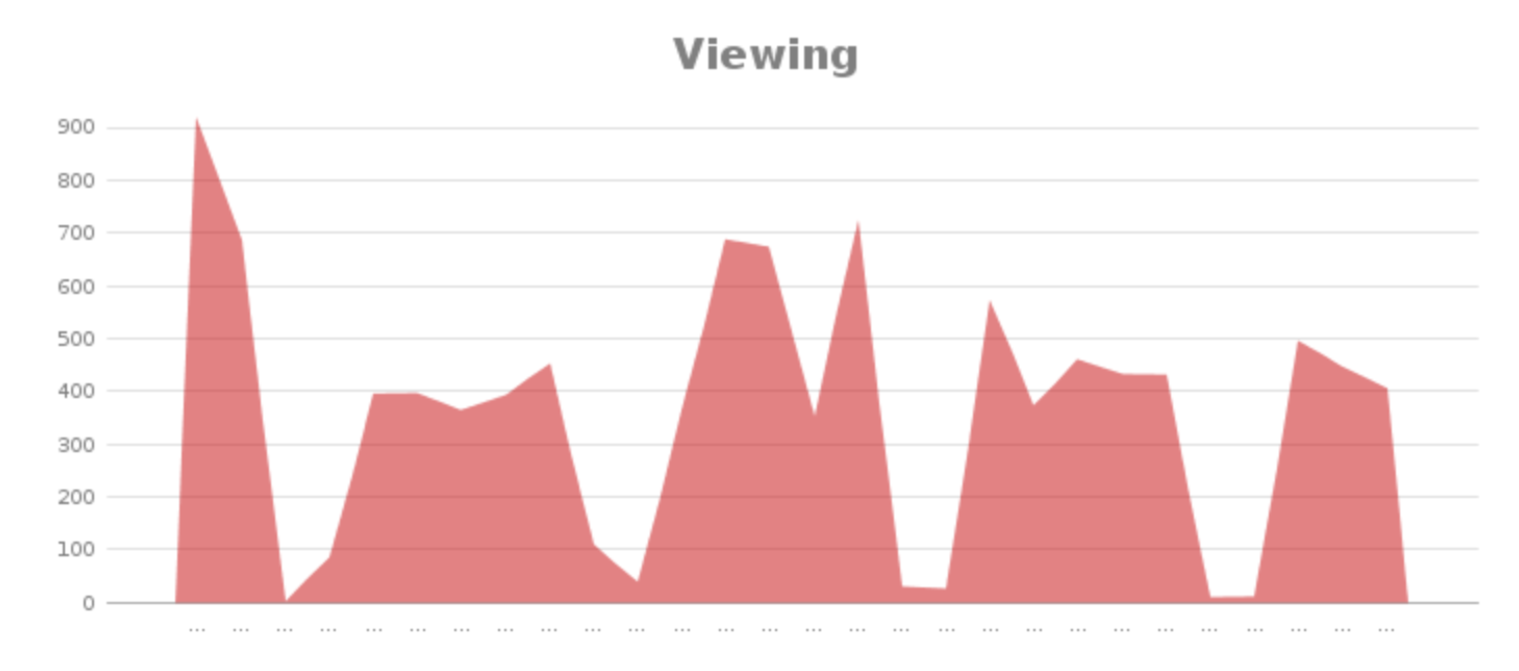
\includegraphics[scale = 0.6]{Bilder/StatsFebView.eps}
\caption{Übersicht über alle eingesehenen Einträge des Monats Februar.}
\label{StatsFebView}
\end{center}
\end{figure}
\\\\
Die Statistiken die durch das \textit{Confluence Usage Stats Plugin} aufgestellt wurden, sollen lediglich für den Monat Februar als Abbildung dargestellt werden. Die Abbildung \ref{StatsFebView} stellt dabei die gelesenen oder betrachteten Einträge dar (Viewing), verteilt auf den gesamten Monat Februar. Abbildung \ref{StatsFebEdit} beschreibt wie viele Einträge erzeugt oder bearbeitet wurden (Editing) und die Abbildung \ref{StatsFebSpaces} zeigt eine Übersicht der \textit{Confluence Spaces} an.  
\\
\begin{figure}[h!]
\begin{center}
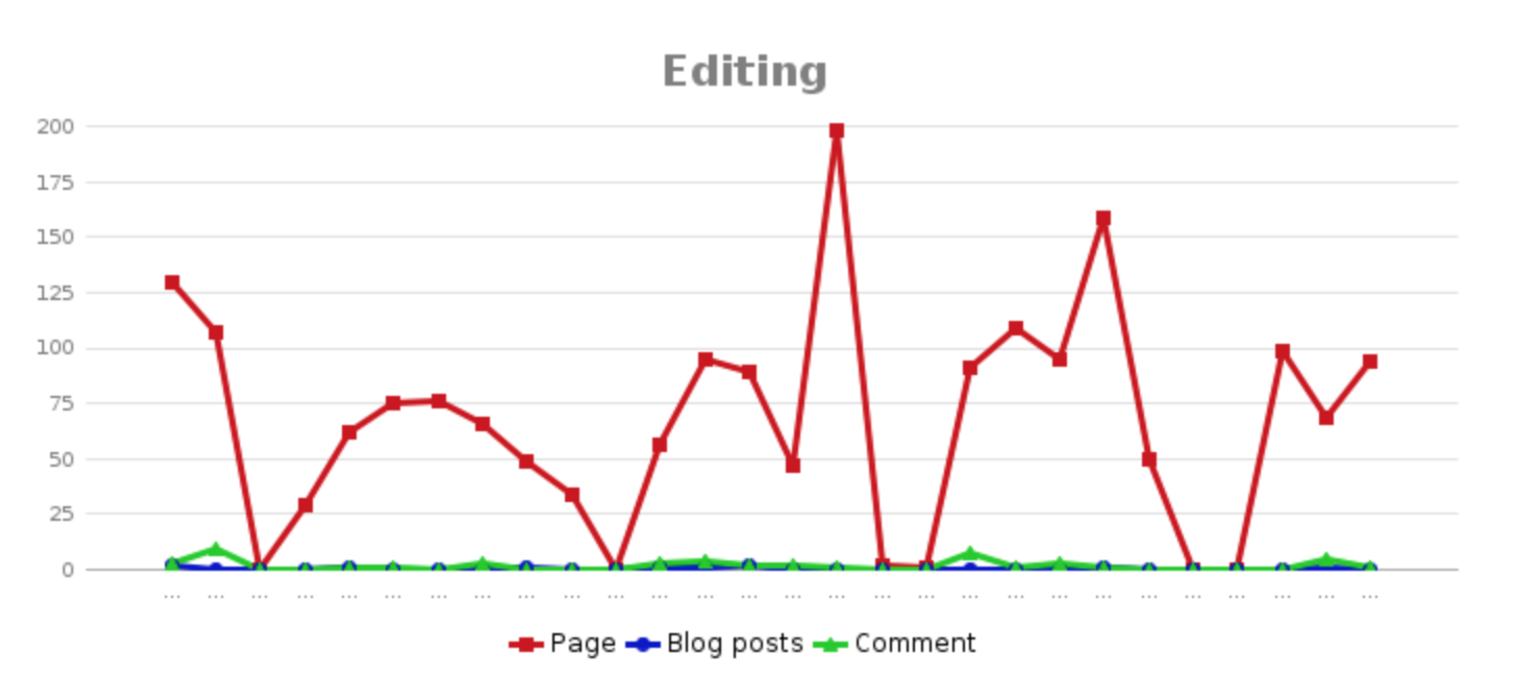
\includegraphics[scale = 0.6]{Bilder/StatsFebEdit.eps}
\caption{Aufführung aller bearbeiteten oder erstellten Einträge des Monats Februar.}
\label{StatsFebEdit}
\end{center}
\end{figure}
\\
Außerdem zeigt Abb.\ref{StatsFebEdit} ebenfalls an, wie viele \textit{Blogbeiträge} und \textit{Kommentare} im gesamten Monat geschrieben wurden. Wie anhand dieser Abbildung zu erkennen ist, bestätigt sich unsere in der Umfrage getroffene Annahme, dass die Kommentar-Funktion von Confluence von den Anwendern nicht verwendet wird. Dadurch sollte nochmals verdeutlicht worden sein, dass diese Funktion im weiteren Vorgehen vernachlässigt werden kann.
\\\\
\begin{figure}[h!]
\begin{center}
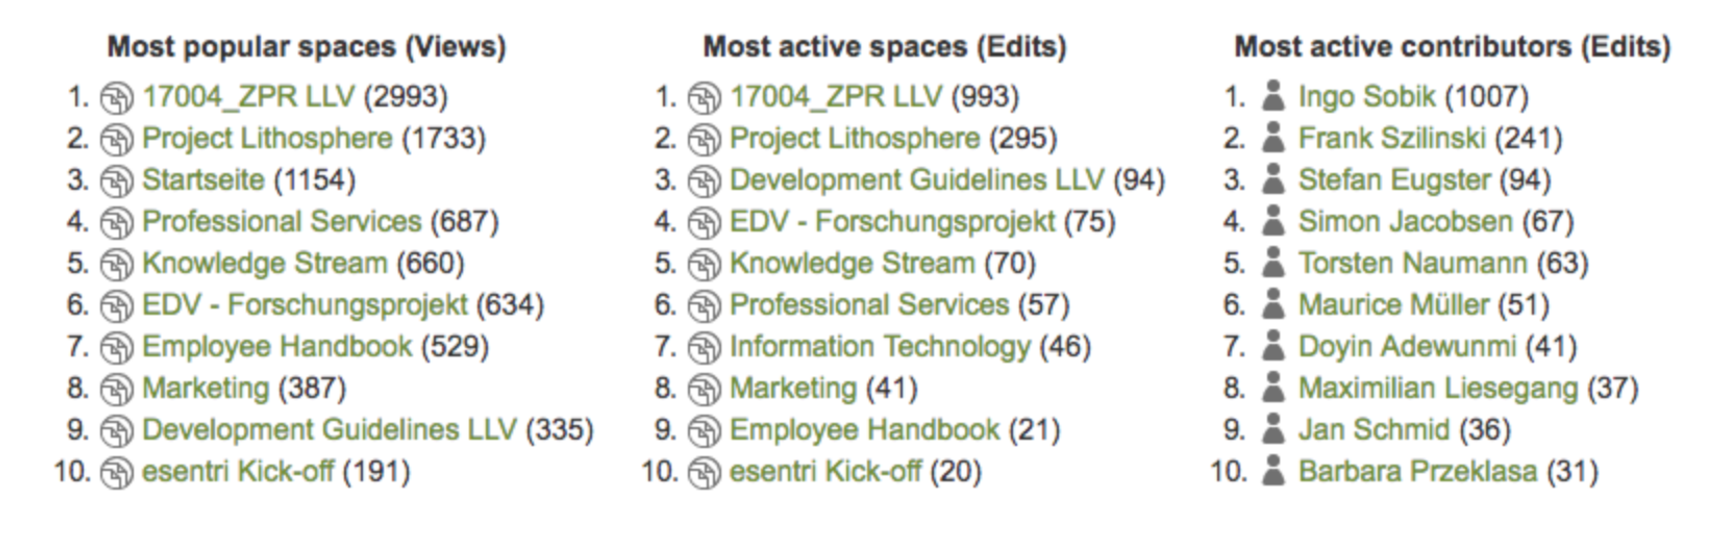
\includegraphics[scale = 0.5]{Bilder/StatsFebSpaces.eps}
\caption{Darstellung der am häufigsten bearbeiteten Spaces im Februar.}
\label{StatsFebSpaces}
\end{center}
\end{figure}
\\
An dieser Stelle sollen noch auf ein paar Punkte aufmerksam gemacht werden. Die \textit{Viewing-Statistik} (Abb.\ref{StatsFebView}) führt alle Einträge auf, die Aufgerufen wurden. Es lässt sich durch diese Statistik nicht bestimmen, ob die Einträge aber auch wirklich komplett durchgelesen oder ob sie nur versehentlich aufgerufen wurden. Außerdem wird beim Erstellen und Editieren eines Eintrages automatisch der Eintrag aufgerufen, somit wird durch das \textit{Editing} immer das \textit{Viewing} ausgelöst. Desto mehr Einträge also bearbeitet werden um so mehr steigt die Anzahl der Views. 
\\\\
Die Geschäftsmetriken für die Views und für die Edits lassen sich nun aus den Statistiken ablesen und zusammenfassen. Die Ergebnisse dieser Zusammenfassung sind in Tabelle \ref{ViewKennzahlenFeb} bis \ref{EditKennzahlenFeb} aufgeführt. Die Geschäftsmetriken für die gesamten Monate Februar und März sollen nun genutzt werden, um die durchschnittlichen Views und Edits am Tag zu bestimmen.
\begin{table}[htb]
\begin{center}
\begin{tabular}{|c|c|c|}\hline
\multicolumn{3}{|c|}{\textbf{Februar}} \rule{0pt}{15pt}\\
\hline
\rule{0pt}{15pt} \textbf{Views} & \textbf{Tage} & \textbf{Geschäftsmetrik} \\ 
\hline
\rule{0pt}{15pt} ca. 9600 & 20 & ca. 480 Views/Tag \\
\hline
\end{tabular}
\caption{Geschäftsmetrik der Views für Februar.}
\label{ViewKennzahlenFeb}
\end{center}
\end{table}
\\
\begin{table}[htb]
\begin{center}
\begin{tabular}{|c|c|c|}\hline
\multicolumn{3}{|c|}{\textbf{Februar}} \rule{0pt}{15pt}\\
\hline
\rule{0pt}{15pt} \textbf{Edits} & \textbf{Tage} & \textbf{Geschäftsmetrik} \\ 
\hline
\rule{0pt}{15pt} ca. 1870 & 20 & ca. 93 Edits/Tag \\
\hline
\end{tabular}
\caption{Geschäftsmetrik der Edits für Februar.}
\label{EditKennzahlenFeb}
\end{center}
\end{table}
\\
Somit haben wir nun die konkreten Kennzahlen der Views und Edits pro Tag ermittelt. Diese Zahlen repräsentieren den aktuellen Ist-Zustand. Mit den Verantwortlichen bei esentri hat man sich nun darauf geeinigt, mit der gamifizierten Confluence Anwendung eine Verbesserung dieser Zahlen von mindestens 10\% anzustreben. Das angestrebte Ziel von 10\% würde dafür sorgen, dass es mehr als 500 Views und mehr als 100 Edits am Tag gibt. Unser angesetztes Ziel von 10\% mag zunächst gering erscheinen, die meisten Gamification Projekte scheitern aber an unrealistischen Geschäftszielen \cite{gamificationDefinition}. Daher ist es besonders wichtig die Geschäftsziele so zu gestalten das sie realistisch, erreichbar und ausdrücklich vermerkt sind.

\subsubsection{Vereinen von Player Goals und Geschäftszielen}
Nun sind sowohl die Ziele der Player (Anwender) und die Ziele der Firma bekannt. Im letzten Schritt dieser Phase müssen die Ziele von Player und Firma miteinander abgeglichen und vereint werden. Dabei ist es für die erfolgreiche Umsetzung einer Gamification-Anwendung wichtig, sich auf die Schnittmenge beider Parteien (Player, Organisation) zu konzentrieren \cite{gamificationDefinition}. Dafür ist es nicht erforderlich, alle Ziele umzusetzen. Für die Gamifizierung der Confluence Wiki sollen die unterschiedlichen Ziele nebeneinander stehend aufgeführt werden.
\begin{description}
   \item[Player Goals:]~\par
   \begin{itemize}
      \item Player wollen Inhalte schnell eintragen. 
      \item Player wollen schnell entscheiden, ob Inhalte vorhanden sind, die sie suchen.
      \item Player wollen, dass ihre Beiträge gelesen werden.
   \end{itemize}
\end{description} 
\begin{description}
   \item[Business Objectives:]~\par
   \begin{itemize}
      \item Die Views sollen um 10 \% gesteigert werden. 
      \item Die Edits sollen um 10 \% gesteigert werden.
   \end{itemize}
\end{description}
Im direkten Vergleich sieht man, die Unterschiedlichkeit beider Parteien. Diese unterschiedlichen Ziele müssen nun vereint und aufeinander abgestimmt werden. Für diese Abstimmung der Ziele wurde kein Verfahren oder Prozess entdeckt bzw. recherchiert der einem Designer oder Entwickler bei der Bewertung und Anpassung der Geschäftsziele und Player Goals unterstützt. Somit liegt die Entscheidungsgewalt, wie die Ziele aufeinander abgestimmt werden, allein beim Designer oder Entwickler.
\\\\
Ein Hinweis zur Gestaltung der gemeinsamen Ziele (Shared Goals) kann aus einem Interview von Brian Burke, Autor des Buches \textit{Gamify}, entnommen werden.
\\\\
\enquote{\textit{One of the most common characteristics is that any gamified solution that's going to be successful invariably focuses on enabling players to achieve their goals. And by doing so achieving the organizational goals, but the organizational goals are really a consequence of motivating players to achieve their goals}} \cite{Kapko14}.
\\\\
Durch diese Aussage wird nochmals deutlich, wie wichtig es ist, die Player in den Mittelpunkt des Design-Prozesses bei gamifizierten Anwendungen zu setzen. Die Geschäftsziele werden also dadurch erreicht, dass die Player wiederum ihre Ziele verfolgen und erreichen. Folglich muss der Fokus also wieder auf die Player Goals und die Player selbst gerichtet werden. Vergleichen wir also die voraussichtlichen Absichten unserer Player mit den Geschäftszielen.        
\\\\
Es liegt wohl auf der Hand, dass es nicht das Interesse des Players ist, mehr Inhalte in die Wiki einzutragen und dadurch mehr Zeit und Arbeit zu investieren. Zumindest nicht ohne einen bestimmten Grund wie z.B den Auftrag eine Dokumentation zu schreiben. Jedoch gaben die Player an, dass sie durch die Verbesserung des Editor-Layouts von Confluence ihre Inhalte schneller erfassen könnten, wenn dieser angepasst werden könnte. Ein schnelleres Erfassen von Inhalten bedeutet aber nicht nur, dass Einträge in die Wiki in weniger Zeit vorgenommen werden können. Es bedeutet auch, dass mehr Inhalte in gleicher Zeit generiert werden können. Wenn diese Vermutung zutrifft, würde das für uns heißen, dass die Player Goals \textit{Inhalte schneller einzutragen} eine Steigerung von Edits in der Confluence mit sich bringen könnte. Ob damit unsere Grenze von einer 10 \% Steigerung erreicht wird, kann zu diesem Zeitpunkt noch nicht ermittelt werden und muss im ersten Testlauf der gamifizierten Wiki geprüft werden.
\\\\
Beim Erfassen von Inhalten in Confluence ist es ohnehin schwer, eine Steigerung der Edits zu erreichen. Da nicht regelmäßig neue relevante Erkenntnisse, die eben in die Wiki eingetragen werden sollten, gewonnen werden. Dadurch wird das Erreichen unseres Geschäftszieles deutlich erschwert. Diese Tatsache lässt sich auch über eine verbesserte und gamifiziertere Confluence Anwendung nicht verändern.    


















  
\newpage
\listoftables
\listoffigures
\newpage
\bibliography{library,library2}

\end{document} 